\documentclass[10pt,a4paper,twoside,titlepage]{report}
%\usepackage[utf8]{inputenc}
\usepackage{amsmath}
\usepackage{amsfonts}
\usepackage{amssymb}
\usepackage{graphicx}
\usepackage{subfig}

\usepackage{hyperref}
\usepackage{frontespizio}
\usepackage[english]{babel}
\usepackage{outlines}
\usepackage[output-decimal-marker={,}]{siunitx}
\usepackage{physics}
\usepackage{xcolor}

\usepackage[left=2cm,right=2cm,top=2cm,bottom=2cm]{geometry}
\usepackage[toc,page]{appendix}
\usepackage[compat=1.1.0]{tikz-feynman}
\usepackage{wrapfig}
\author{Adriano del Vincio}

\tikzfeynmanset{every blob = {minimum size = 3mm}}

\begin{document}

\begin{frontespizio}
\Logo[2.5cm]{Simbolo/cherubino_pant541.eps}
\Istituzione{Università di Pisa}
\Dipartimento{Fisica "Enrico Fermi"}
\Corso[Laurea]{Fisica}
\Titoletto{Tesi di laurea}
\Titolo{Commissioning and first data analysis \\ of the Mainz radius experiment.}
\Candidato[562946]{Adriano Del Vincio}
\Relatore{Prof. Francesco Forti \\ Prof.ssa Concettina Sfienti}
\Annoaccademico{2022-23}
\end{frontespizio}

\tableofcontents


\begin{abstract}
short introduction
\end{abstract}


\chapter{Physics Motivation for Neutron Skin Thickness Measurement} \label{intro}
\commento{
\begin{itemize}
\item explain neutron skin thickness.
\item connection to neutron stars radious, and neutron stars description.
\item Equation of state (EoS) for high density nuclear matter.
\item Parity-violating scattering experiment for extracting neutron skin thickness.
\item mention the weak form factor.
\item Transverse asymmetry as background for Parity-violating experiment. 
\item Mention the other experiment, like PREX, that measure zero $A_{n}$ for Lead.
\end{itemize}}

\section{The Mainz Radius Experiment}

The Mainz Radius Experiment (MREX), at the Mainz nuclear physics institute, is an experimental campaign with the aim of investigating the complex nature of atomic nuclei. The strong force, whose presence was first speculated by Yukawa in 1935, is responsible of a broad range of phenomena: from characteristic of atomic nuclei, the compositions of baryons and meson to the exotic structure of Neutron stars. So, the field of nuclear physics provides many answers to fundamental questions in other fields of physics. In particular the neutron stars, that are one of most interesting astrophysical object in the universe, are ideal to study and test theories of dense matter, providing so many connection between particle physics, astrophysics and nuclear physics. It can be surprising to think that, despite a difference of so many order of magnitude, neutron rich nuclei and neutron stars have the same basic physics, enshrined by the the Equation Of State (EOS) of neutron rich matter. The Equation Of State represents the fundamental relation between the state variables as temperature, energy, pressure and neutron-proton asymmetry. Specifically, the final goal of the MREX experiment is to determine an important parameter of the EOS, that is the slope of the symmetry energy at saturation density $L$. This parameters is important for the determination of the radius of the neutron stars, but it is also responsible of a peculiar characteristic shown by heavy nuclei: the neutron skin thickness $\delta r_{np}$. The neutron skin thickness is a phenomena that affect heavy nuclei which consists in the accumulation of the excess of neutrons near the surface of a nucleus. Such skin thickness is strongly sensitive to $L$, so an accurate determination of the neutron skin provides significant constrains on the value of $L$ which in turn is used as an input to many theoretical models of the structure of the neutrons stars.
The determination of $\delta r_{np}$ presents considerable difficulties. While $r_{p}$ is known with high accuracy, thanks to the electrons elastic scattering experiment which involves electromagnetic force, the determination of $r_{n}$ has traditionally relied on hadronic experiments which involves proton-nucleus scattering, $\pi^{0}$ photo-production, $\alpha$ and $\pi$ nucleus scattering. Those process suffer from large and often uncontrolled theoretical uncertainties that compromises the extraction of the neutron density. The most promising method, that is the least model dependent, is the parity-violating electron scattering. In this reaction longitudinal polarized electrons are elastically scattered off unpolarized target. This method consist in the measurement of the asymmetry between right and left handed electrons:

\begin{equation}
A_{pv} = \dfrac{\sigma_{R} - \sigma_{L}}{\sigma_{R} + \sigma_{L}}
\end{equation}

This process is dominated by the exchange of a virtual photon, which is sensitive to charge form factor, and a $Z_{0}$ boson, that is sensitive to the weak form factor. Because of the fact that the weak charge of the neutrons is $Q_{w} = 0.99$ and the weak charge of the proton is $0.04$, the weak form factor contains the information on the neutron density, necessary to measure $\delta r_{np}$. The MREX experiment will measure the neutron skin thickness via the parity violating scattering at the new MESA accelerator.

\section{Nuclear Equation of State (EOS) and Neutron Skin Thickness}

\commento{In this section we have to explain what is the neutron skin thickness and why this parameter is related to the Equation of State for nuclear matter (in particular, the slope of the Symmetry energy in the semiempirical mass formula). Then, explain the parallelism between Neutron stars and Nuclear matter (the share the same EOS), and underline the relation between radius of the neutron stars and EOS.}

During the 30s of the last century, a considerable part of the scientific community was concentrated in the study of the structure of atomic nuclei. The discovery that every atoms has a positive charged nucleus dates back to 1908, with the famous Rutherford experiment, where alpha particles scatter from a thin gold foil. In the following years, especially with the birth of quantum mechanics in the second half of the 1920s, significant progress were made in the knowledge of atomic nuclei and their properties. In 1935, a significant contribution was given by Carl Friedrich von Weizsäcker, that proposed the semi-empirical mass formula, to approximate the mass of an atomic nucleus. Although some refinements have been made over the years, the general structure of the formula is the same today. 
The model proposed by Weizsäcker is the application of the liquid-drop model for nuclear matter, where the Nucleus is described as drop of protons and neutrons, that are assumed to be incompressible and are held together by a nuclear potential. The semi-empirical mass formula states that the mass of a nucleus is given by 

\begin{equation}
m = Zm_{p} + Nm_{n} - \frac{E_{B}(N,Z)}{c^{2}}
\end{equation}

An important terms is the binding energy $E_{B}$, that contains 5 parameters:

\begin{equation}
E_{B} = a_{V}A -  a_{s}A^{\frac{2}{3}} - a_{c}\dfrac{Z^{2}}{A^{\frac{1}{3}}} -a_{asym}\dfrac{(N - Z)^{2}}{A} + \delta(N,Z)
\end{equation}

The first two terms $a_{V},a_{s}$ are taken from the liquid drop model, and are the volume energy and the surface energy. The volume term represent the energy due to the interaction of each nucleon with the other nearby nucleons. This term is proportional to $A$, that is the number of nucleon of the nucleus, which is proportional to the volume, hence the name. The second term represent is the surface energy, and it is a correction to the volume energy. The volume energy assume that each nucleon interact with a constant number of nearby nucleons, but this is not true if we consider the external protons and neutrons, because they have less neighbors to interact with. This correction terms is then proportional to $A^{\frac{2}{3}}$, that is the also proportional to the surface area. 
The third term $a_{c}$ denote the binding energy correction due to the repulsion between protons. The fourth term is $a_{asym}$, the asymmetry term, and it is proportional to the asymmetry between neutrons and protons. The theoretical justification for this terms is due to the Pauli exclusion principle. Neutrons and protons are distinct type of particles, and occupy different quantum states. Because neutrons/protons are fermions, they can't occupy a state with the same quantum numbers, therefore higher energy states are progressively filled. If there is an asymmetry between neutrons and protons, for example the number of neutrons is greater than the number of protons, some neutrons will be in higher energy states respect to the protons. The imbalance between the nucleons causes the energy to be higher respect to the situation with the same number of protons and neutrons. 
The last term the pairing term, and describes the effect of spin coupling, and has positive/negative values for even or odd N,Z. 
We want to focus on the fact that the liquid-drop model has the underlying assumption that the nucleons are incompressible. Because of this it's well defined the concept of saturation density, the fact that the density, at first order, is almost constant and independent of mass number A.
In the context of neutron stars, it's more useful to take the thermodynamic limit in which the number of nucleons and Volume are taken to infinity. The binding energy per nucleons can be written as:

\begin{equation}
\epsilon (\rho_{0}, \alpha) = -\frac{E_{B}}{A} = -a_{V} + a_{asym} \dfrac{\rho_{n} - \rho_{p}}{\rho_{n} + \rho_{p}}
\end{equation}

In reality, this simple equation is only an approximation, because the nuclear matter doesn't behave like an ideal liquid drop, and it is not incompressible. To describe the response of the nuclear matter to density variation, as well as temperature, etc... we need the equation of state (EOS) of the system, that binds these quantities thermodynamically. For neutron stars, the EOS depends on $\rho$, the conserved baryon density, and neutron-proton asymmetry $\alpha$, in the ideal limit of $T = 0$:

\begin{equation}
\epsilon (\rho,\alpha) = \epsilon_{snm} (\rho, \alpha = 0) + \alpha ^{2} S(\rho) + O(\alpha ^{4})
\end{equation}

The energy density is expanded in a power series of $\alpha = \dfrac{\rho_{n} - \rho_{p}}{\rho_{n} + \rho_{p}}$. No odd power of $\alpha$ appears in the expansion, because the strong force doesn't depend on the isospin, or in other words, neglecting electromagnetic interaction and weak interaction, the equation of state depends only on the relative asymmetry between neutrons and protons, it doesn't matter if such an asymmetry is biased towards protons or neutrons.
The terms $S(\rho)$ is the symmetry energy, and it represents the cost of converting symmetry nuclear matter ($\alpha = 0$) to pure neutrons matter, as the case of neutron star. Now we can proceed considering the saturation density. A further expansion around the saturation density $\rho$ is necessary:
	
\begin{equation}
\begin{split}
S(\rho) &= J + L \cdot \dfrac{\rho - \rho_{0}}{3 \rho_{0}} + \dfrac{1}{2} K_{sym} \cdot \biggl(\dfrac{\rho - \rho_{0}}{3 \rho_{0}}\biggl)^{2} \\
\epsilon _{smn} (\rho) &= \epsilon_{0} + \dfrac{1}{2}K_{0} \biggl(\dfrac{\rho - \rho_{0}}{3 \rho_{0}} \biggl)^{2} 
\end{split}
\end{equation}

Several new terms appear in this expression:
\begin{itemize}
\item $\epsilon_{0}$ is the energy per nucleon for symmetric matter at saturation density.
\item $J$ is the symmetry energy at saturation density.
\item $L$ is the slope of the symmetry energy.
\item $K_{0}$ is the incompressibility coefficient for symmetry matter. 
\item $K_{sym}$ is the incompressibility coefficient for the symmetry energy.
\end{itemize}

In this expression appears for the first time $L$, the slope of the symmetry energy. This is a key component of the EOS, whose values is an important parameter to determine the radius of neutron star. $L$ quantifies the difference between the symmetry energy at saturation (as in the nuclear core) and the symmetry energy at lower densities, as in the nuclear surface.$L$ is also related to the pressure $P$ at saturation density. Giving the EOS in term of $\rho,\alpha$, the pressure is given by:

\begin{equation} \label{eq:Pressure}
P = \rho^{2} \dfrac{\partial \epsilon(\rho, \alpha)}{\partial \rho}
\end{equation} 

A formal demonstration of this relation is given in the appendix (\commento{mettere referenza}). We know write $\epsilon_{snm}$ making explicit all the dependencies:

\begin{equation}
\epsilon (\rho, \alpha) = (\epsilon_{0} + \alpha^{2} J) + \alpha^{2}Lx + \frac{1}{2} (K_{0} + \alpha^{2}K_{sym})x^{2}
\end{equation}

we substitute $x = \dfrac{\rho - \rho_{0}}{3 \rho_{0}}$. Considering pure neutron matter $\alpha = 1$, the pressure at saturation density $P_{0}$ can be easily computed withe the formula (\ref{eq:Pressure}). The result is the following:

\begin{equation}
P_{0} \simeq \dfrac{1}{3}\rho_{0} L
\end{equation}

From this expression we learn that the slope of the symmetry energy is essential to determine the pressure for densities near saturation. The contribution of the symmetric term $\epsilon_{snm}(\rho)$ vanishes, and at first order the pressure depends only on $L$. Because of this, it becomes more and more clear the link between $L$ and the neutron skin thickness. Let's consider the case of the $^{208}Pb$, with ad excess of 44 neutrons. Placing the excess of neutrons in the surface of the nucleus is discouraged by surface term $a_{S}$, which tends to minimize the area. However, if the excess of neutrons is placed in the core of the nucleus, this is increase the symmetry energy $S(\rho)$. In the end the neutron skin is the result of the competitions between the surface tension and the slope of the symmetry energy.
 Measurement of the neutron skin have been performed by the PREX collaboration at Thomas Jefferson National Accelerator Facility in Virginia \cite{Abrahamyan:2012gp}, however the precision attained was insufficient to distinguish between the various competing models which describe the relation between $\delta r_{np}$ and $L$ (\ref{fig:LvsR}). Despite this, theoretical predictions states that there is a strong correlation between these two quantities, in the following plot we show how different theoretical models, with different values of $L$ used as input, predict the values of $\delta r_{np}$ for lead:

\begin{figure}[hbtp]
 \centering
 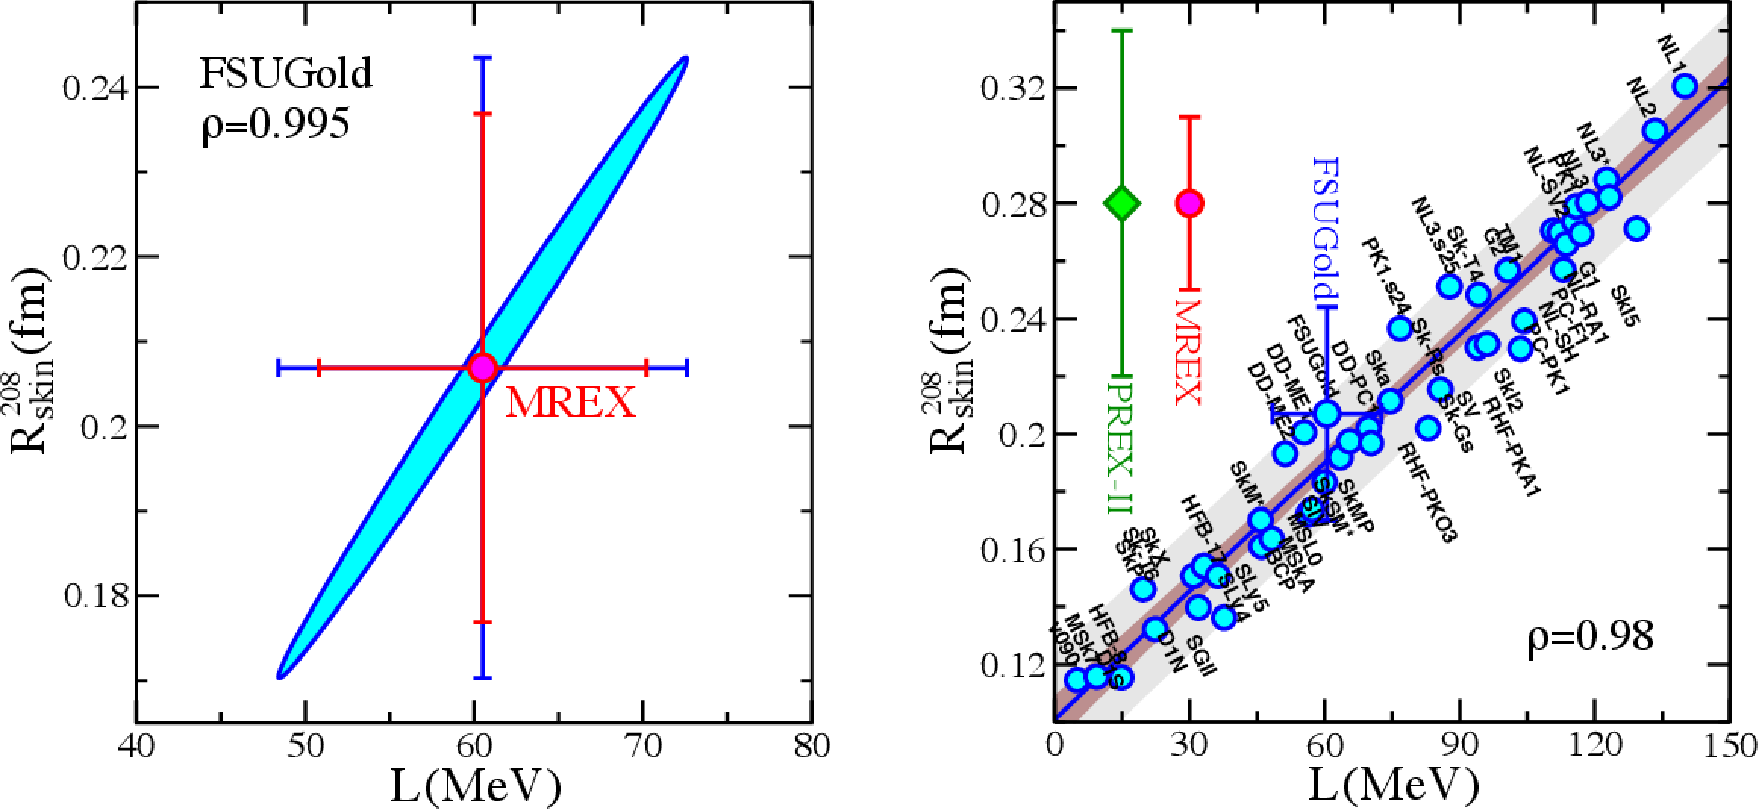
\includegraphics[width=0.75\textwidth]{Introduzione/LvsR.pdf}
 \caption{Neutron skin thickness of $^{208}Pb$ as a function of the slope of the symmetry energy $L$. The error bars represent $\pm \SI{0.06}{\femto \meter}$ and $\pm \SI{0.03}{\femto \meter}$ for the future experiments of PREX-II and MREX. Notice the different scale for x and y axis: the uncertainty for the neutron skin measurement is amplified for the correspondent values of $L$ }
 \label{fig:LvsR}
 \end{figure}
 
A strong linear correlation is evident, and so it is clear that measuring the neutron skin is a promising way to measure $L$. 

\subsection{Neutron Star Radius}


\section{Parity-violating Scattering Experiment}

The parity violating electron scattering seems to be the most promising method in order to determine the neutron-skin thickness for $^{208}Pb$. The choice of lead is due to the significant neutron excess and stability of lead nuclei ($^{208}Pb$ is a double magic nucleus). The advantage of this method is that it is free from the many uncertainties associated to strong interaction. The main disadvantage is the necessity to accumulate large statistics, because the reaction are mediated by the weak interaction, that produce a smaller amplitude compared to electromagnetic and strong interaction. 
The parity violating scattering is high sensitive to the neutron density because, as mention above, the weak charge of the neutron is higher compared to the weak charge of the proton.
In this reaction, longitudinally polarized electrons are elastically scattered off a lead target. The important quantity to determine is the parity violating asymmetry $A_{PV}$, the difference in cross section between the scattering of right and left handed electrons. 

\begin{equation}
A_{PV} = \dfrac{\sigma_{R} - \sigma_{L}}{\sigma_{R} + \sigma_{L}}
\end{equation} 

The theoretical calculation of $A_{PV}$ concern the interference between the exchange of virtual $\gamma$ and $Z^{0}$. In the Born approximation $A_{PV}$ is directly proportional to the weak form factor, and it is given by the formula below:

\begin{equation}
A_{PV} \simeq \dfrac{G_{F} Q^{2}}{4 \pi \alpha} \cdot \dfrac{Q_{W} F_{W}(Q^{2})}{Z F_{ch}(Q^{2})}
\end{equation} 

$G_{F}$ is the Fermi constant, $Q^{2}$ is the transferred momentum, Z and $Q_{W}$ is the electric and weak charge of the nucleus. The Charged form factor of the lead nucleus is known with high accuracy (precision of 0.02 \%), so in this limit the only quantity that is unknown is $F_{W}(Q^{2})$. In the long wavelength approximation, the weak form factor at single value of momentum transfer is given by:

\begin{equation}
F_{W}(Q^{2}) = \frac{1}{Q_{W}} \int \rho_{W}(r) \dfrac{sin(Qr)}{Qr} d^{3}r = (1 - \frac{Q^{2}}{6} R^{2}_{W} + \frac{Q^{4}}{120}R^{4}_{W} + ...)  
\end{equation}

The form factor is normalized in such a way that $F_{W}(Q^{2} = 0) = 1$. The weak charge radius correspond to $R^{2}_{W} = -6 \frac{\partial F_{W}}{\partial Q^{2}}\Bigr|_{\substack{Q^{2} = 0}}$. Now it is clear that parity-violating experiment are a promising method to extract information about neutron density. The effort is represented by the small values of $A_{pv}$ asymmetry. Typical values are on the order of $1 \, ppm$ or less, for lead target. This requires high statistic to reduce the uncertainty of the measurement. 
In 2012 PREX collaboration measured for the first time through parity-violating experiment the neutron skin, the values is:

\begin{align*}
\delta r_{np} = 0.33^{+0.16}_{-0.18} \SI{}{\femto \meter}
\end{align*}

The error associated to this first measurement is not enough small to provide significant constraints on the values of $L$. Because of this, the MREX experiment has the objective of measuring the neutron radius of lead with a precision of $0.5 \%$  ($\pm \SI{0.03}{\femto \meter}$). This high precision is needed to decrease the uncertainty associated to L. For example, the left plot in \ref{fig:LvsR}, shows the correlation between the neutron skin thickness of $^{208}Pb$ and the slope of the symmetry energy as predicted by FSUGold model (\cite{Fattoyev_2011}). With a precision of $\pm \SI{0.03}{\femto \meter}$, $L$ is determined with $\pm \SI{12.1}{\mega \electronvolt}$.

\section{Transverse Asymmetry}

\commento{Here we have to introduce the aim of this thesis: the transverse asymmetry is a source of background for the parity-violating experiments. Furthermore the theory is not working well for some nuclei ($^{208}Pb$), so mention PREX paper about the last measurement on carbon and lead, the problem that they measure $0$ transverse asymmetry.}

The parity-violating scattering has numerous advantages for extracting the neutron-skin thickness of nuclei. However, the asymmetry to measure is rather small. The important effort is to reduce at most possible systematic effects that can alter the result of the measurement. One of the principal source of background for the measurement of $A_{PV}$ is a different process that concerns transverse polarized electrons. The different polarization of the electrons produce an asymmetry that is called beam normal single spin asymmetry, or transverse asymmetry $A_{n}$. Because such asymmetries are typically one order higher that the parity-violating ones, a small normal component of the beam polarization during parity-violating experiment can produce a systematic effect that alter the final result. The subject of this thesis is the measurement of transverse asymmetry $A_{n}$ for carbon target, performed at MAMI, the Mainz microton accelerator. The choice of carbon target is due to the fact that the transverse asymmetry for carbon is well known and already measured at MAMI; the expected asymmetry is roughly $20 \, ppm$ , thus it is particularly suited for a commissioning of the new experimental setup. In this section don't introduce physics of this process, that will be extensively treated in the next chapter. However, we mention that such measurement are challenging because they require calculation of box diagrams with intermediate excited states \cite{Gorchtein_2008}.
After the determination on $A_{n}$ for $^{12}C$, the next step of the MREX experiment will be the determination of the \transv for $^{208}Pb$. As already mentioned, this is mandatory to constrain the systematic effects of PV experiment. However, it is also interesting because for last measurement performed by PREX \cite{HAPPEX:2012fud} the \transv for $^{208}Pb$ target is compatible with zero, and this is in striking disagreement with the theoretical predictions. 


\chapter{Transverse Asymmetry} \label{transv}

\begin{itemize}

\item Physics behind the $A_{n}$ asymmetry, dependence on $Q^{2}$, the formula $\frac{\sigma_{\uparrow} - \sigma_{\downarrow}}{\sigma_{\uparrow} + \sigma_{\downarrow}}$
\item state of the art of the Exp.
\item Model description: so scattering amplitude, theoretical prediction
\item Expected error $ \delta A_{t} $
\item open question: problems with lead, dependence of $E_{beam}$, dependence from Z, Z/A
\end{itemize}

\section{Description of the process}

{\bfseries Explain the scattering process we are studying (at least one figure to visualize the kinematics of the scattering). Mention the link between this process and time-reversal operator. Add two figures for elastic and inelastic scattering.} 

The Beam Normal single spin asymmetry, which we will refer for brevity as Transverse asymmetry, originates from the interference of two scattering process. For the purpose of this thesis, we will present the case of electron scattering against a spin $0$ target \cite{Gorchtein_2008}.
To understand why the interference of this two scattering amplitude give rise to an asymmetry, we first have to look at the kinematic of the experiment: 

\begin{figure}[hbtp]
\centering
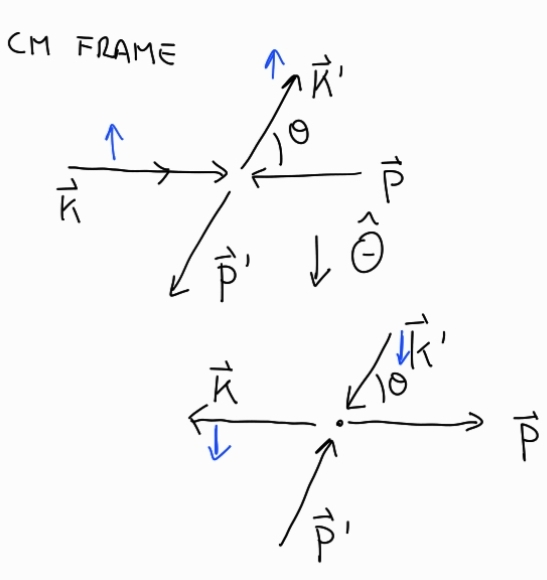
\includegraphics[width = 0.4\textwidth]{figures/Kinematic.jpg}
\caption{•}
\end{figure}

Where all the momenta are measured respect to the center of mass frame. In the figure we can confront the two situation before and after applying the Time-reversal operator, $\hat{\Theta}$. Looking at the picture we can understand that : 

\begin{itemize}
\item Before applying $\hat{\Theta}$, we have the incident electron with $\vec{k}$ momenta and the nucleus with $\vec{P}$ momenta, after applying $\hat{\Theta}$ we have that the incident/outgoing electron and the incident/outgoing nucleus are exchanged.
\item The $\hat{\Theta}$ operator acts also on the spin of the electron. Because we are considering process where the spin doesn't flip, the two situations are not equivalent.
\item Considering that the process is elastic, the kinematic is the same, taking $\vec{p}$ and $\vec{k}$ as the initial particle momenta, or $\vec{p}'$ and $\vec{k}'$. 

\end{itemize}

The time-reversal operator seems to connect the two different cases of UP and DOWN polarized electron. Our effort is to measure the asymmetry between the two cross section:

\begin{equation}
A = \frac{\sigma_{\uparrow} - \sigma_{\downarrow}}{\sigma_{\uparrow} + \sigma_{\downarrow}}
\end{equation}

And it's particularly clear that a non-zero asymmetry depends on how the time-reversal act on the elastic amplitude of the process. \\
With this idea, let's see in more detail the $\hat{\Theta}$. We know that $\hat{\Theta}$ is an antiunitary operator that can be always seen as:

\begin{align*}
\hat{\Theta} = U \cdot K
\end{align*} 
Where $U$ is an unitary operator, while $K$ is the complex conjugation operator that generates the complex conjugate of each coefficient in front of it. If we cosider a ket describing a system we have that:

\begin{equation}
Kc \ket{\alpha} = c^{*} K \ket{\alpha}
\end{equation}

Now, let's consider $H$ as the hamiltonian of our system. We want to apply the $\hat{\Theta}$ operator. We can now use the assumption that the hamiltonian consist of two term, which correspond to the two different scattering process. Because of the electromagnetic interaction conserve $CP$, so also $T$ is conserved, we know in advance that each piece of the hamiltonian commute with $\hat{\Theta}$. Now let's see what happen for an hamiltonian which has an imaginary part:

\begin{equation}
H = H_{R} + i H_{Im} \quad ; \quad \hat{\Theta} H \hat{\Theta}^{-1}= \hat{\Theta}H_{R} \hat{\Theta}^{-1} + \hat{\Theta} i H_{Im} \hat{\Theta}^{-1} \Rightarrow H_{R} - i H_{Im} \neq H
\end{equation}

what we understand from these simpe calculation is that to give rise to an asymmetry, we expect an imaginary part of the scattering amplitude different from zero.\\
At the $\alpha$ leading order, the two process of the electron-Nucleus scattering that give rise to the asymmetry involve the exchange of one-photon-exchange (OPE) and two-photon-exchange (TPE). The Feynman diagrams that describes the processes are the following: 

\begin{figure}
\[
\feynmandiagram [scale = 1, transform shape][baseline = (h), horizontal = d to j]{
	a [particle = \(e^{-}\)] -- [fermion, thick] c -- [fermion, thick ] f -- [fermion, thick] g [particle = \(e^{-}\)],
	c -- [photon, edge label = \(\gamma\)] d [blob],
	f -- [photon, edge label = \(\gamma\)] j [blob],
	h [particle = \(C^{12}\)]-- d -- [fermion, thick] j -- k [particle = \(C^{12}\)] ,
	};
\qquad
\feynmandiagram [scale = 1, transform shape][ vertical = c to d]{
	a [particle = \(e^{-}\)] -- [fermion, thick] c -- [fermion, thick] g [particle = \(e^{-}\)],
	c -- [photon, edge label' = \(\gamma\), momentum = {[arrow style = red]\(k\)}] d [blob],
	h [particle = \(C^{12}\)] -- [fermion, thick] d -- [fermion, thick] j [particle = \(C^{12}\)],
	};
\]
\caption{TPE and OPE diagrams in electron nucleus scattering.}
\end{figure}


A seguire come si scrive l'ampiezza per il termine elastico ed inelastico, aggiungere in appendice come viene fatto l'integrale sullo spazio delle fasi e stop. 



\subsection{Elastic scattering}

{ \bfseries Write the amplitude for the elastic (how to manipulate expression, maybe in the appendix). }


\subsection{Inelastic scattering}

Explain how it's possible to compute the inelastic expression, what kind of approximations are used (optical theorem...) 

\subsection{Model description}
Present the theoretical formula for the Transverse asymmetry, and comment on energy, Z, Z/A depencencies adding together the elastic and inelastic contributions, we end with the following formula which describes the process \cite{PhysRevLett.121.022503}:

\begin{equation}
A_{N} = C_{0} \cdot log(\dfrac{Q^{2}}{m_{e}^{2} c^{2}}) \dfrac{F_{Compton}(Q^{2})}{F_{ch}(Q^{2})}
\end{equation}

\section{State of the Experiment}

Write down the formula $\frac{\sigma_{\uparrow} - \sigma_{\downarrow}}{\sigma_{\uparrow} + \sigma_{\downarrow}}$. Hints at how to measure the Transverse asymmetry (remember to mention we have a polarized beam against a unpolarized target). Explain the expected error for the recostructed asymmetry. Furthemore talk about the last mesurements obtained by the other collaborations, an outlook of the current situation. Maybe add also how we proceed to measure the transverse asymmetry, so the structure of the event, polarities patterns...
\bigskip

We have seen so far how the Transverse Asymmetry is related to the interference between two scattering amplitude, and the theoretical model used to describe the process. The goal from an experimental point of view is to measure this quantity. The challenge is to obtain a valid measure of $A_{n}$, which is of the order of $20$ part per million (ppm), taking into consideration all the possible effects that can interfere. To measure $A_{n}$, the straighfoward method is to prepare an electron beam, with polarized electron, and send it to a fixed target. The scattered electrons are then collected by a detector placed at a certain angle, and now it's possible to obtain the trasverse asymmetry applying the formula:

\begin{equation}
A_{} (Q,p) = \dfrac{N_{\uparrow}(Q) - N_{\downarrow}(Q)}{N_{\uparrow}(Q) + N_{\downarrow}(Q)} \cdot (\frac{1}{p})   
\end{equation} 

where we have explained the dependence on the transmitted impulse, on the degree of polarization of the beam.
In an experiment of this type, several requests are necessary to have an effective data acquisition:

\begin{itemize}
\item The accelerator must produce a polarized beam, stable over the time, with an high polarization percentage, in order to amplify the effect.
\item The Beam energy needs to be quite stable, and should not depend on the Polarization state of the electrons. A change in the Beam energy associated with the polarization state, can lead to a different count rate for $N_{\uparrow}$ and $N_{\downarrow}$, would make a contribution that would be added to that of the physical process
\item The beam must be correctly alligned with the target, and stable. Again if the position of the target changes accordin to the polarization of the electrons, it will produce another contribution to the total asymmetry.
\item The beam current should not depend on the polarization state of the electrons. If the beam source depends on the polarization, we will have a difference in the event rate and then another false asymmetry.
\item it's necessary to reject possible double elastic scattering events, which may contribute to the total asymmetry. 
\end{itemize}

All this demands can be satisfied with an accelerator that has stabilization devices with great precision and that can sustain high beam intensities. This last request is necessary to accumulate enough statistics to measure the transvere asymmetry with an accuracy about 1 ppm, in view of the future PV experiments. We can quantify how the statistical error varies according to the amount of data avaible. With the quite general assumption that the measured rate $N_{\uparrow,\downarrow}$ are gaussian distributed variables, we can compute the expected variance of $A_{n}$:

\begin{equation}
Var[A_{n}] = \dfrac{1 - A^{2}}{N_{\uparrow} + N_{\downarrow}} 
\end{equation}

This is the variance associated to a single measurement of the transverse asymmetry. As is well known, the variance scales as $\frac{1}{n}$ as $n$, the number of measures, increases.
Beacause the $A_{n}$ is expected to be quite small, we can approximate the above formula:
\begin{align*} \label{eq:Error}
V[A_{n}] = \dfrac{1}{2N \cdot n}
\end{align*}

The error associated to the recostructed asymmetry is the square root of the above quantity. If we impose that the error must be $\le 1ppm$ we can easily obtain that the quantity $n\cdot N$:

\begin{align*}
n\cdot N \le \frac{1}{2} \cdot 10^{12}
\end{align*} 

We will see later that achievable rates $N_{\uparrow,\downarrow}$ are in the range (20000,100000) for a carbon target. This number can not be increased at will by acting on the beam current. The first reason is obivios: the accelator and the beam source can handle only a certain amount of electrons before loosing their characteristics, furthermore a beam with great intensity for an extended periods of time can damage the carbon target, up to the risk of melting it. 
Another idea might be to increase the thickness of the target, to take advantage of the larger cross section. However this does not take into account that by doing so the number of double scattering event is increased. To avoid this the scientific community that deals with these nuclear physics measurements respect the convenction that the target thikness should be less than the $10 \%$ of the radiation lenght of the material.

\chapter{Experimental setup} 

\paragraph{} The Mainz Microtron Accelerator (MAMI), where the experiment is set up and the transverse asymmetry is measured, is briefly described in this chapter.  The description of the beam monitors used to measure the beam parameters is given a special consideration. Following an overview of the experimental hall, the detectors and the electronic devices used to acquire and process the data. 

\section{Overview of the Experiment} \label{FirstDescription}

To measure the Beam Normal Single Spin Asymmetry, a polarized beam of $ \SI{570}{\mega \electronvolt}$ is directed towards a  $^{12}C$ target that is $\SI{10}{\milli \meter}$ thick. The detectors are made up of two fused-silica bars coupled to 3 (detector B) and 8 (detector A) PMTs, which are used to gather the Cherenkov light released when an electron passes through the fused-silica. The detector are placed inside the two spectrometers of the A1 hall. Due to the high beam current ($ \SI{20}{\micro \ampere}$), which is above their operating
limits, the standard detectors of the spectrometers are not employed in this experiment. The experiment aims to measure the cross-section asymmetry between the two electron spin orientations. The PMT signals are collected and digitalized by the \textbf{NINO} board, after a threshold selection, and sent to the A1 control room computer, where the DAQ program collect the data together with all the data coming from the beam monitors. The produced  binary files are later analyzed by the analysis program, which is a significant part of the work done in the framework of the thesis. 
The data collected are divided in \textit{events} made by 4 \textit{sub-events} in sequence. Each event corresponds to a temporal window of $\simeq \SI{80}{\milli \second}$, where each sub-event is $\SI{20}{\milli \second}$ long. This structure into sub-events reflects the polarization sequence of the beam.
Unlike the majority of experiments in high energy physics, an event is not a single interaction, but is made by all the electrons interacting with the detectors during the specified time interval. The PMT counts and the beam monitor values are saved for each sub-event, along with their time length (measured in clock cycles by the NINO electronic board) and other values which are required to process beam monitor data. The general structure of the event is the shown in figure \ref{fig:EventStructure} 

\begin{figure}[hbtp] 
\centering
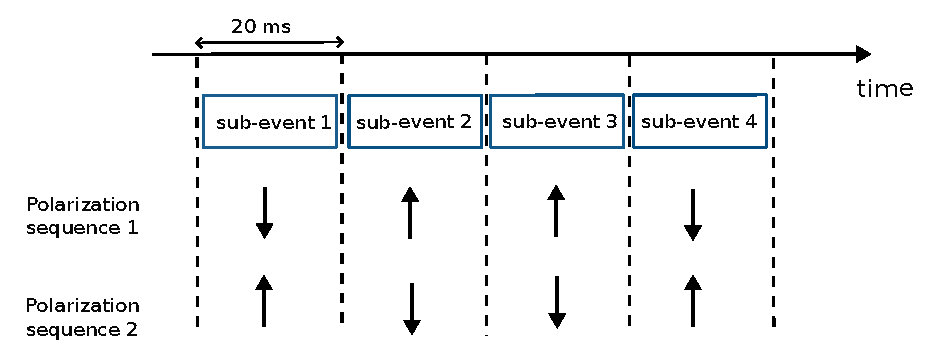
\includegraphics[width = 0.75\textwidth]{ExperimentalSetup/EventStructure.pdf}
\caption{General structure of the event. The gate-length of each event is synchronized with the power grid frequency, to reduce possible effects of $\SI{50}{\hertz}$ noise.}
\label{fig:EventStructure}
\end{figure}

The particular choice of $\SI{20}{\milli \second}$ for each sub-event is made to reduce undesirable effects relate to the power grid frequency ($\SI{50}{\hertz}$). The gate-length of each sub-events is synchronized with the period of the power grid frequency: this ensures that an entire oscillation of the current takes place within the same sub-event. This cancels out the $\SI{50}{\hertz}$ noise and avoid to produce effects between nearby sub-events.

An event corresponds to a single measurement of $A_{n}$, defined as the asymmetry between the $\uparrow$ and $\downarrow$ sub-events. To avoid the creation of false asymmetries by correlated noise or other external sources the polarization states are concatenated following the two patterns $\uparrow, \downarrow, \downarrow, \uparrow$ and $\uparrow, \downarrow, \downarrow, \uparrow$. Which sequence an event belongs to is decided using a De Bruijn sequence. A De Bruijn sequence of order n is defined as a cyclic sequence where every sub-sequence of length $n$ appears only once. We have two different polarization pattern, the ones shown in the figure, that can be represented as $1$ and $0$. For this experiment, the De Bruijn sequence is of order $n = 6$ bits, corresponding to all the possible sequences of $1$ and $0$ with a length equal to $6$, which are $64$ different sub-sequence.
It is possible to demonstrate that the number of exactly $N_{bruijn}$ sequences is: 
\begin{align*}
N_{bruijn} = \frac{(k!)^{k^{n-1}}}{k^{n}}
\end{align*}
If we substitute in the formula above $k=2$ and $n = 6$, we have a total of $\simeq 67 \cdot 10^{6}$ different sequences. The seed of the De Bruijn sequence is generated with a pseudo random number generator, and the sequence is used to select between $\uparrow,\downarrow,\downarrow, \uparrow$  and $\downarrow,\uparrow,\uparrow,\downarrow$. At this point it could be objected why so much care is taken in choosing randomly the two sequences. At a first glance is certainly easier to select one of the two polarization pattern and reproduce it for every sub-event. However, this would not protect from systematic effects that arise from electronic or beam noise with frequencies similar to the frequency of the polarization pattern. For instance electronic noise with  $ f \simeq \SI{10}{\hertz}$ could in principle increase the rates for one polarizations state and decrease the other one. The adopted solution to reduce effects of this type is to randomize the pattern selection. Besides this, there is another reason why a De Bruijn sequence is useful. During each polarization flip, we observe a short, transient reduction of the beam current. This reduction in the beam intensity has more influence on patterns where there are more inversion of the polarization respect to the other. With a De Bruijn sequence we ensure that we have a identical number of pairs of patterns, meaning that:


\begin{itemize}
\centering
\item $25\%$ : $\uparrow,\downarrow,\downarrow, \uparrow$ ; $\uparrow,\downarrow,\downarrow, \uparrow$
\item $25\%$ : $\downarrow,\uparrow, \uparrow,\downarrow$ ; $\downarrow,\uparrow, \uparrow,\downarrow$
\item $25\%$ : $\downarrow,\uparrow, \uparrow,\downarrow$ ; $\uparrow,\downarrow,\downarrow, \uparrow$
\item $25\%$ : $\uparrow,\downarrow,\downarrow, \uparrow$ ; $\downarrow,\uparrow, \uparrow,\downarrow$
\end{itemize}


In the top rows we have 4 inversions, while in the two lower rows we have 5 inversions.
Other details of the experiments are presented in this chapter. In the next section the operating principles of MAMI electron accelerator are discussed.

\section{Statistical Uncertainty}

We can quantify how the statistical error varies according to the amount of data available. With the assumption that $N_{\uparrow,\downarrow}$ are gaussian distributed variables, we can compute the expected variance

\begin{equation}
Var[A_{n}] = \dfrac{1 - A^{2}}{N_{\uparrow} + N_{\downarrow}} 
\end{equation}

For a single measurement of the $A_{n}$. For multiple $n$ measurements, the variance scales as $\frac{1}{n}$.
Because $A_{n}$ is expected to be smaller respect to 1, we can approximate the above formula:
\begin{equation} 
V[A_{n}] = \dfrac{1}{2N \cdot n}  \label{eq:Error}
\end{equation}

The error associated to the reconstructed asymmetry is the square root of the above quantity. If we impose that the error must be $\le 1ppm$ we can easily obtain that the quantity $n\cdot N$:

\begin{align*}
n\cdot N > \frac{1}{2} \cdot 10^{12}
\end{align*} 

We will see later that achievable rates $N_{\uparrow,\downarrow}$ are in the range (20000,60000) counts per event for a carbon target. This number can not be increased at will by acting on the beam current. In the first place there is a limitation on the total charge that the beam source can produce; in addition, a beam with great intensity for an extended periods of time can damage the carbon target up to the risk of melting it. Another idea might be to increase the thickness of the target, to take advantage of the larger cross section. However, by doing so, the number of double scattering events would be increased. To avoid the problem of the double scattering, the nuclear physic community which deals with PV experiments respects the convention that the target thickness should be less than the $10 \%$ of the radiation length of the material.

\section{MAMI}

MAMI is the electron accelerator located in Mainz, which provides a continuous wave \footnote{The electron beam is made by bunches of electrons, in sequence. In MAMI the separation between subsequent bunches is so small that it is not possible, with the available instrumentation, to distinguish it from a continuous flow of particles.}, high intensity, polarized beam for nuclear physics fixed-target experiments. The concept of the Mainz microtron accelerator was developed in the early 1970s, when the researchers of the nuclear physics institute were investigating the possibility of generalizing the concept of the racetrack microtron (RTM), that consists in a linear accelerator (linac) and two deflection magnets ($180^{\circ}$ magnet, see figure \ref{fig:RaceTrackSketch}). The bending magnets make the particles recirculate several times in the linac, and each time they gain energy. MAMI is developed to produce a continuous beam, with energies above $\SI{1}{\giga \electronvolt}$ and beam intensities starting from $\SI{1}{\nano \ampere}$ up to $\SI{100}{\micro \ampere}$.

\begin{figure}[hbtp]

\centering
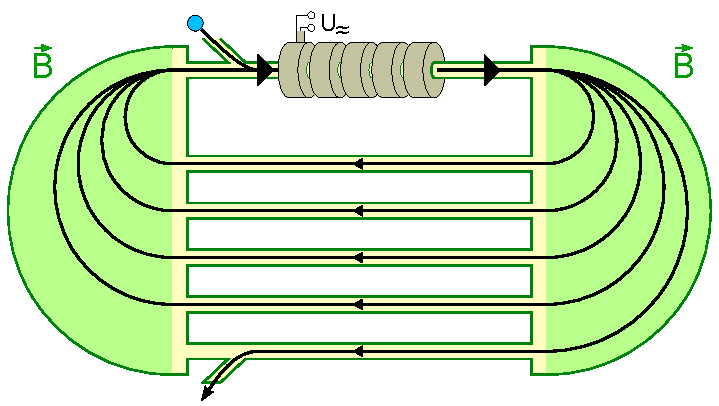
\includegraphics[width = 0.75\textwidth]{ExperimentalSetup/RacetrackMicrotronSketch.pdf}
\caption{Racetrack Microtron. The particles are sent to the linac, and the two deflection magnets make the particles recirculate, until the momenta exceed the capability of the magnetic field.}
\label{fig:RaceTrackSketch}
\end{figure}

A racetrack microtron is characterized by the energy gain per-cycle, $\delta E$, given by the high-frequency electromagnetic field (HF). The energy gain for a single acceleration cavity of the linac is: 

\begin{align*}
\delta E \, = \, e U_{Linac} \cdot cos(\phi)
\end{align*} 

$U_{Linac}$ is the maximum voltage of the linac, and $\phi$ is the phase of the beam relative to the maximum of HF. The beam consist in individual packets (bunches) of electrons, whose rate correspond to the frequency of HF. To be accelerated during each recirculation step, the electron bunches must arrive at entrance of the linac with the correct phase $\phi$. Therefore the electron time of flight per cycle must be an integer or a multiple of the HF period. The time of flight is made of two terms: the first is the time needed to travel in the magnetic field of two $180^{\circ}$ bending magnets, equal to the cyclotron period; the second term is instead given by the straight sections, and remains constant for relativistic motion. 

\begin{equation} \label{eq:TimeofFlight}
T = \dfrac{2 \pi \gamma m_{e} }{qB} + \dfrac{L}{v}
\end{equation}

where $B$ is the magnetic field, $q$ and $m_{e}$ are the charge and mass of the electron, and $L$ is the length of the straight section of the accelerator. The frequency is given by the formula:

\begin{equation} \label{eq:frequency}
f = \dfrac{qB}{2 \pi \gamma m_{e} + \frac{LqB}{v}} 
\end{equation}

From these two equations two conclusion can be drawn:

\begin{itemize}
\item To accelerate slow electrons, with $\gamma = (1,10)$, a magnetic field of $\SI{0.1}{\tesla}$ is used, in order to work with frequencies of ($\SI{2}{\giga \hertz}$,$\SI{4}{\giga \hertz}$), that are easy to control. However with higher energies, and with a small magnetic field, the bending radii is higher and uneconomical.
\item For high energy electrons $\gamma > 10$, to reduce the size of the deflection magnets, it is useful to increase the magnetic field up to $\SI{1}{\tesla}$ of more, with the same band of frequencies $\simeq \SI{}{\giga \hertz}$.
\end{itemize}

This justifies the structure of MAMI: a cascade of microtrons to reach progressively higher energies, with the same acceleration frequency at each stage. In MAMI there is a sequence of 4 different microtrons, that are able to accelerate particle up to $\SI{1.6}{\giga \electronvolt}$. 

\begin{figure}[hbtp]
\centering
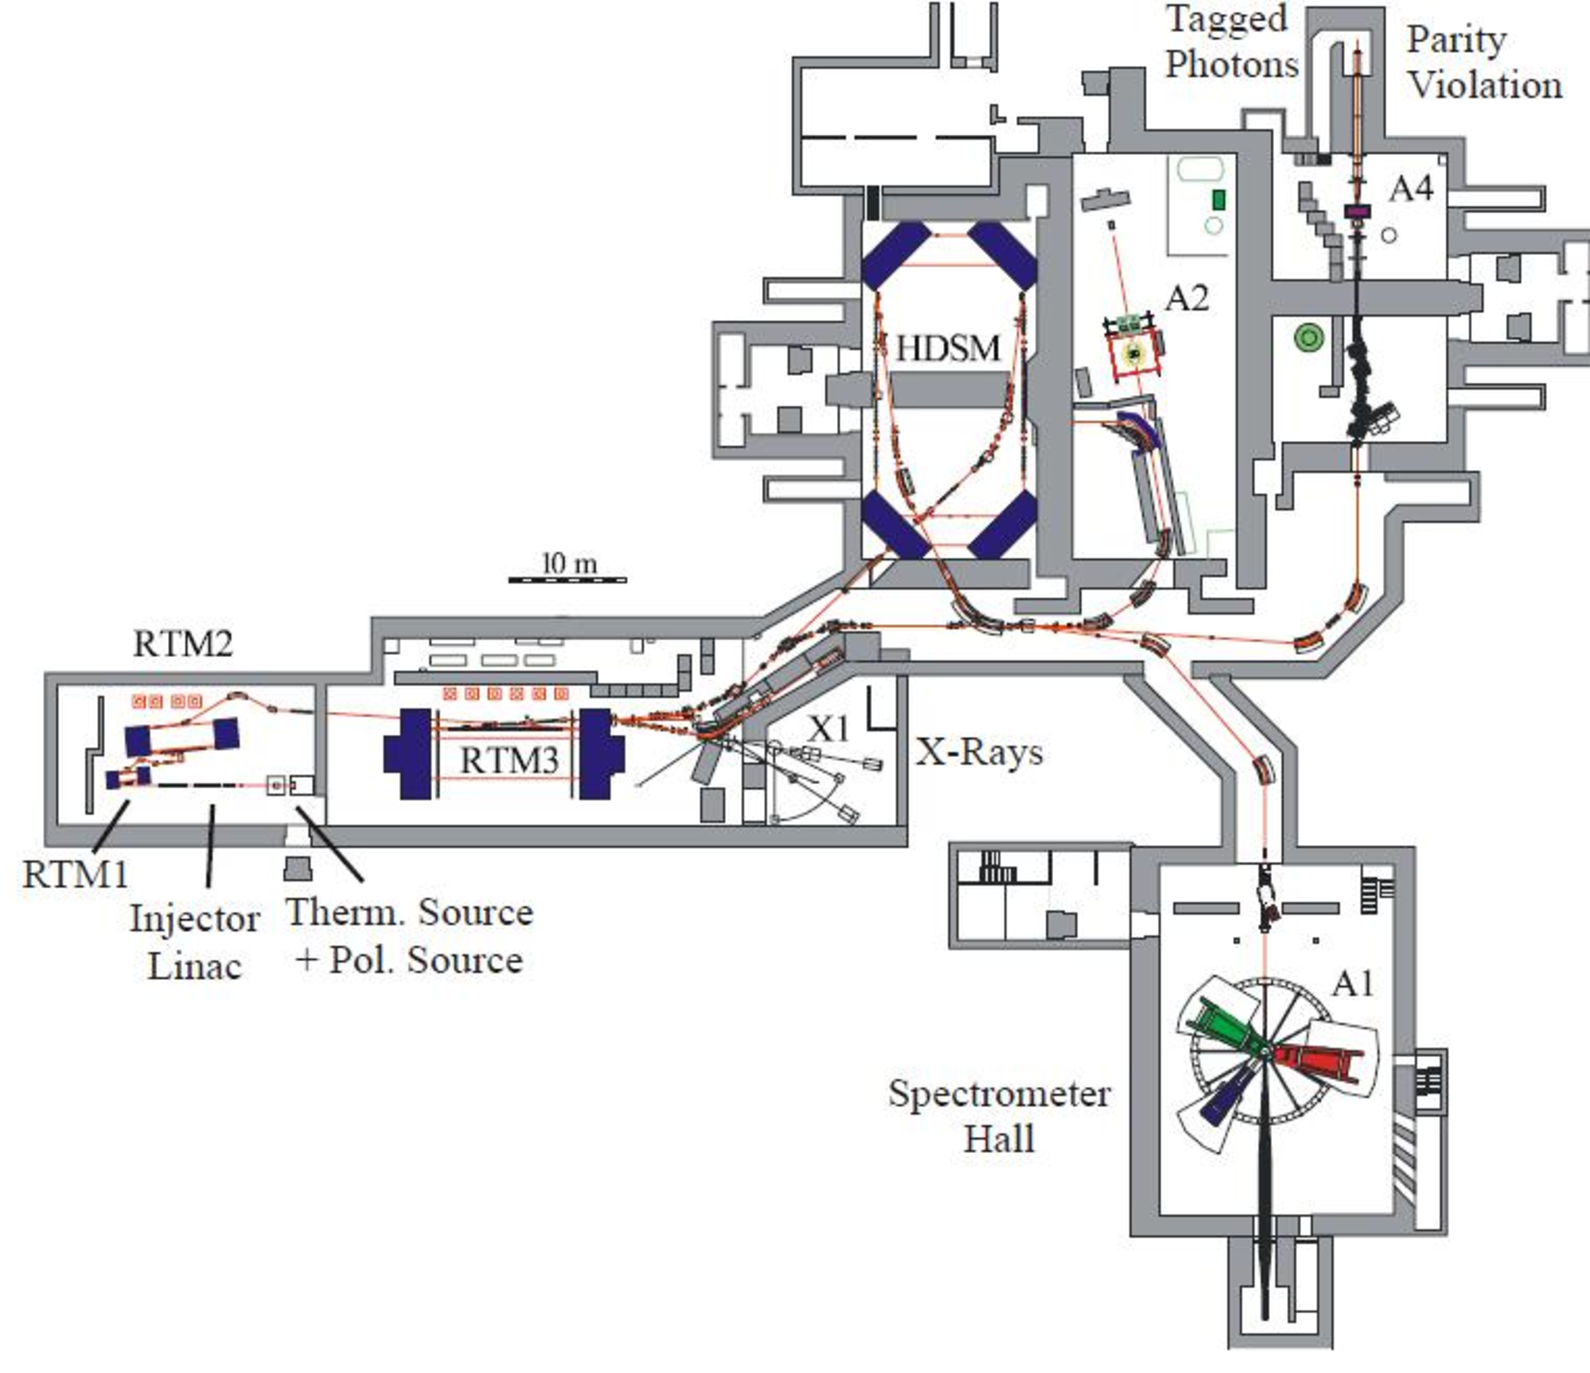
\includegraphics[width = 0.6\textwidth]{ExperimentalSetup/Accelerator.pdf}
\caption{Scheme of the accelerator, with the different experimental halls. A third hall previously used for the A4 experiment, measuring the strange quark content of the proton, is now being used for the novel MESA accelerator and its experiments.}
\label{fig:Accelerator}
\end{figure}

The first stage, shown in figure \ref{fig:Accelerator}, is composed by two small microtrons. The first microtron, RTM1, accelerates the particles up to $\SI{14}{\mega \electronvolt}$ in 18 revolutions. Then the electrons are sent to the RTM2, second microtron that can reach an energy of $\SI{180}{\mega \electronvolt}$. After passing this first stage, the beam is directed towards the RTM3 (race track microtron 3), in the adjacent room, that is large microtron with an end point energy of $\SI{855}{\mega \electronvolt}$. The sequence of RTM1, RTM2 and RTM3 forms MAMI-B, which is operating since 1990-91. A fourth stage, MAMI-C, was built and started operation in 2007. This fourth stage is made by 4 bending magnets, with a bending angle of $90^{\circ}$, and it is designed to achieve energies of $\SI{1.6}{\giga \electronvolt}$. MAMI-C design is different from the other race-track microtrons, and it is not discussed, as it is not necessary for the experiment to reach such high energies.

\begin{figure}[hbtp]
\centering
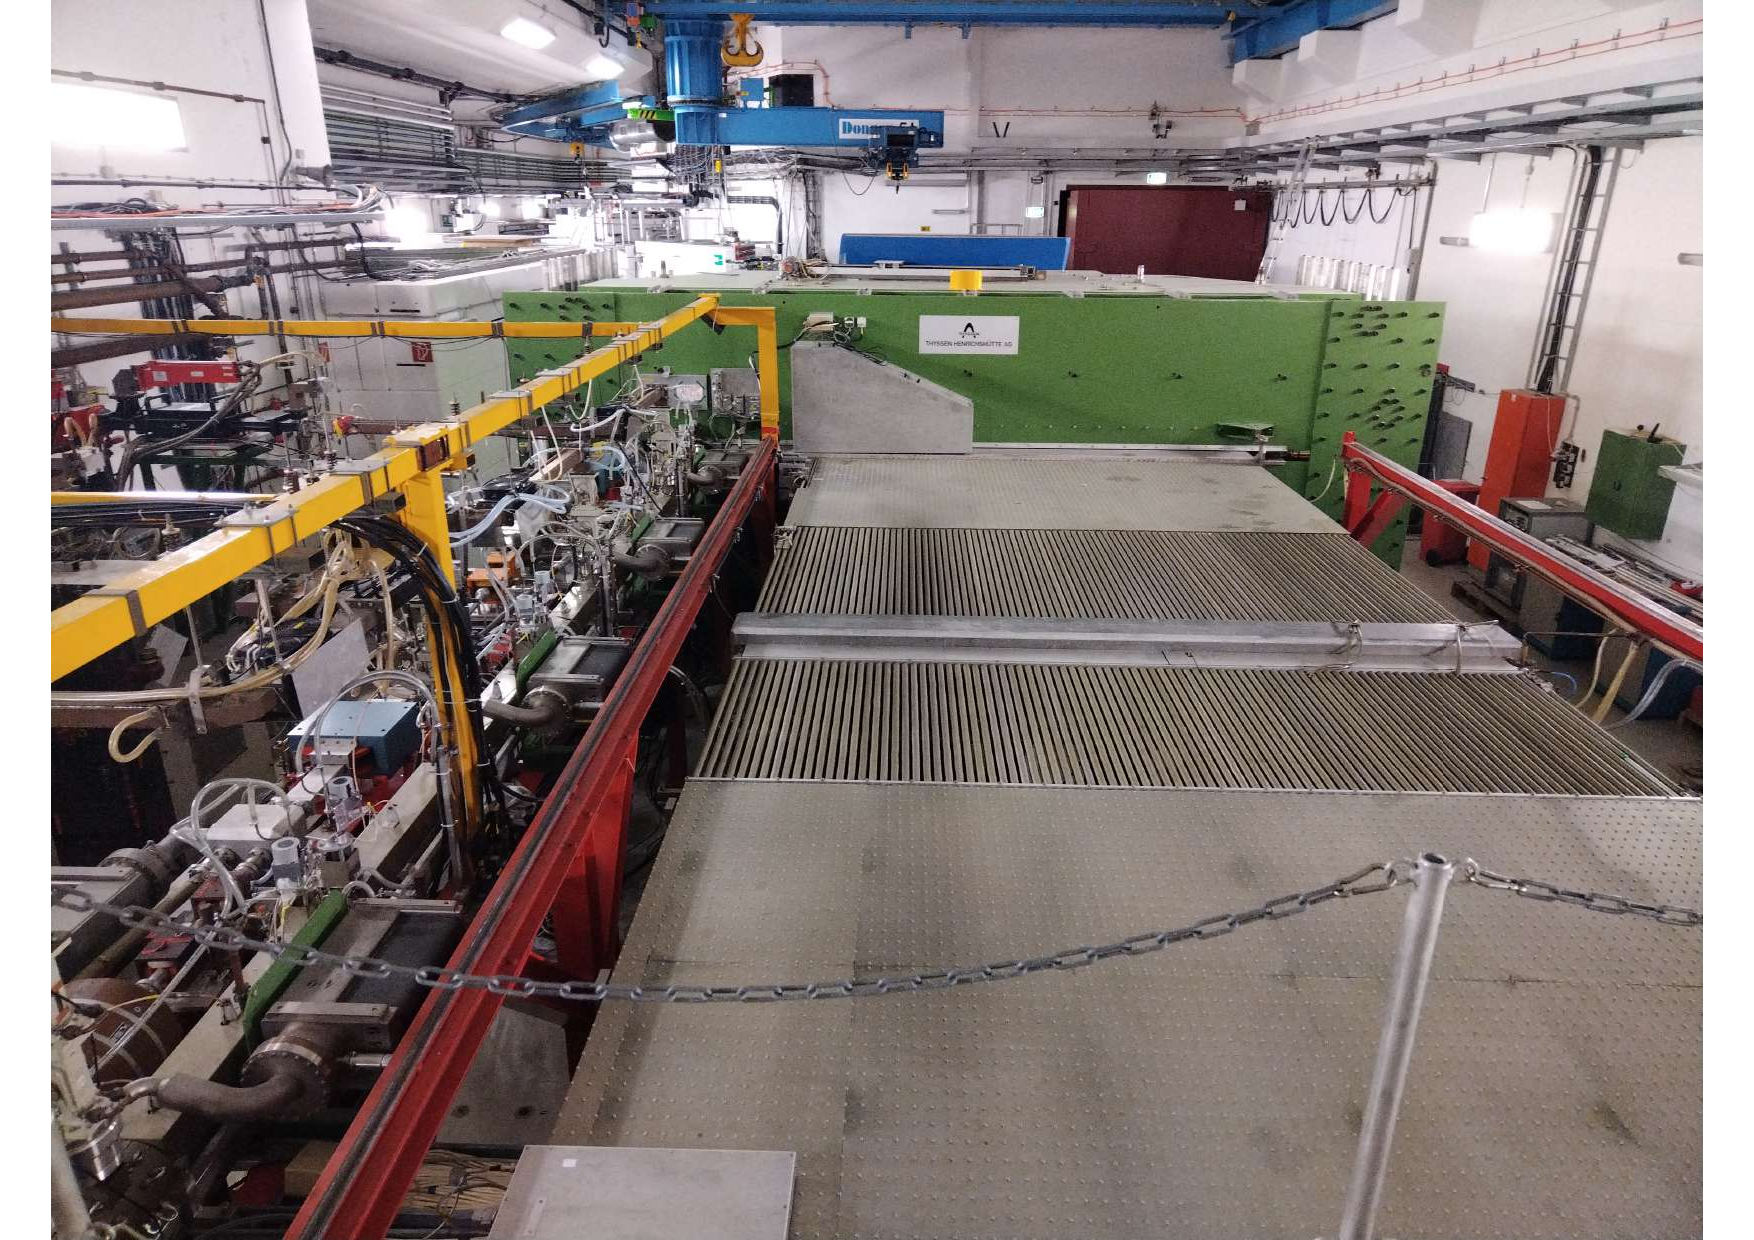
\includegraphics[width=0.75\textwidth]{ExperimentalSetup/Racetrack.pdf}
\caption{Picture of the Racetrack RTM3 in MAMI-B. The Green square at the bottom is one of the deflector magnets, the other one is below the point where the photo was taken. The linac stage is on the left. The tubes at the center of the figure are the paths that the particle cross during the recirculation. The further away from the linac the greater the energy.}
\end{figure}

The operation principles of a microtron is simple to be described. First we consider the gyro-radius for relativist electrons of energy $E$, that is:

\begin{equation}
\qquad r = \dfrac{E \beta}{qcB}
\end{equation}

To have a coherent conditions, we must have that the flight time $\tau = \frac{\lambda}{c}$ of the first recirculation must be an integer multiple of the HF wavelength $\lambda_{HF} = \frac{c}{f_{HF}}$, as shown in equation \ref{eq:frequency}. This means that:

\begin{align*}
\lambda = \tau c =\dfrac{ 2 \pi c r }{\beta c} + \frac{Lc}{v} = \dfrac{2 \pi E}{q B} + L = m \lambda_{HF}
\end{align*}

For the subsequent recirculations, the flight-time at energies $E_{n} = E_{n-1} + \delta E$ must be increased by an integer multiple of HF, too. This lead to a second equation:

\begin{align*}
\dfrac{2 \pi \delta E}{q B} = n \lambda_{HF}
\end{align*}

The minimum gain per cycle is then determined only by the strength of the magnetic field and wavelength $\lambda_{HF}$. The system of these two equations controls the dynamic of the race-track microtrons, and determines the working point of the accelerator.

\subsection{Polarized Beam}

For the beam-normal single spin asymmetry a vertically polarized beam is necessary. At the MAMI electron accelerator it is possible to produce a vertically polarized beam with energy in the range $\SI{180}{\mega \electronvolt} - \SI{855}{\mega \electronvolt}$ \cite{Schlimme:2016rrp}. The procedure to orient the spin vertically is discussed in this section, and the measurement of the degree of polarization is explained. 

The electron source used at MAMI is made by a strained GaAs/GaAsP super-lattice photo-cathode illuminated by circularly polarized light. To alternate the sign of the light polarization, a fast Pockels cell (\cite{Goldstein}) is installed in the optical system of the electron source. The Pockels cell is a wave plate controlled by the electric field, that changes the helicity of the photons impinging on the electrons. A Pockels cell exploits the Pockels effect, that affects crystal with particular characteristics (lack of inversion symmetry). For this type of materials the refractive index is linearly dependent on the applied electric field. By controlling the refractive index, the polarization state of the incident light beam is altered. Since the angular momentum is conserved, the extracted electron carries the same helicity of the incoming photon:
\begin{center}
\begin{equation}
\feynmandiagram [scale = 0.8, transform shape][baseline = (g)]{
	a [particle = \(e^{-}\)] -- [fermion] b  -- [fermion] c [particle = \(e^{-}\)],
	b -- [boson] d [particle = \(\gamma\)],};
\hspace{2cm}
(Jz)_{\gamma} = \pm 1 \qquad (Jz)_{e^{-}} = \mp \frac{1}{2} \rightarrow \pm \frac{1}{2}
\end{equation}
\end{center}

With the fast change of the Pockels cell it is possible to alternate the sign of the polarization. By the insertion of a $\lambda/2$ plate between the laser system and the photo-cathode, the global polarization orientation of the electron beam can be reversed. This is useful because changes directly the sign of the asymmetry measured by the detectors, and allows to identify systematic errors. Usually, two sets of data are taken during an experiment, reversing the orientation of the $\lambda/2$ wave plate. By comparing the results for the two sets of data, the influence of the optical system on the asymmetry measurement is estimated and is used to correct the final result of the asymmetry. However changing the orientation of the $\lambda/2$ wave plate requires a certain amount of time and it is usually done for longer beam time. During the experiment described in this thesis, the $\lambda/2$ wave plate orientation was fixed. 

The beam degree of polarization achieved with the electron source is roughly $P = 80 \% $. The degree of polarization reduces the measured asymmetry:

\begin{align*}
A_{measured} = P \cdot A_{n}
\end{align*}

The electrons extracted by the circular polarized laser are longitudinal polarized. A combination of magnetic fields is needed to rotate $\vec{P}$ from longitudinal to transverse orientation. For this purpose two devices are used: Wien filter and a double solenoid, located in the injection beam line, close to the the optical source, as show in figure \ref{fig:Iniezione}

\begin{figure}[hbtp]
\centering
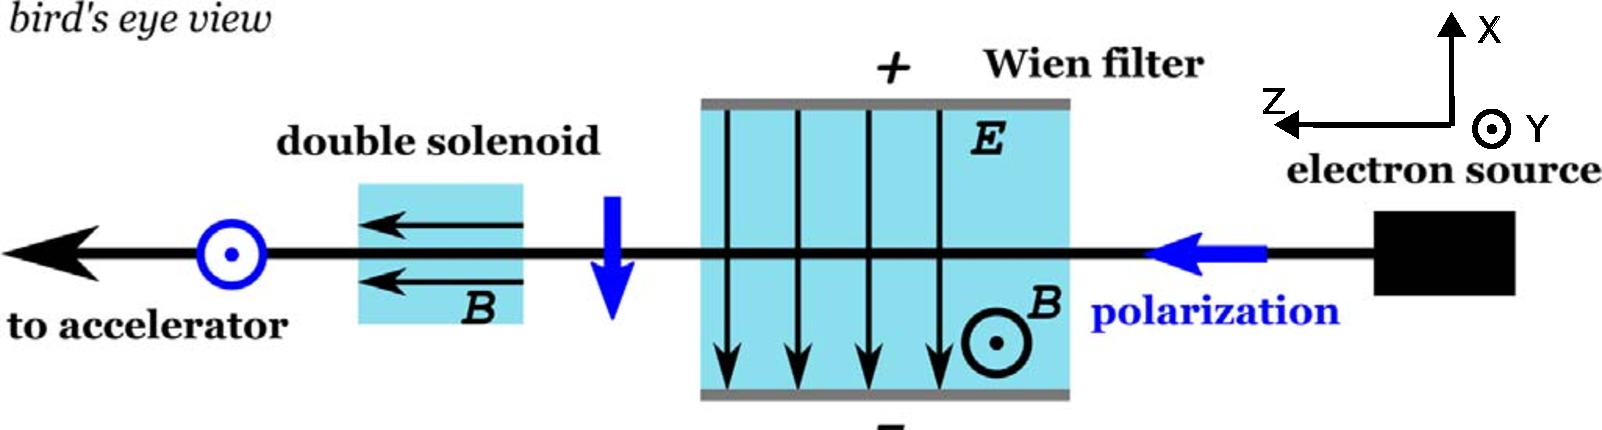
\includegraphics[width = \textwidth]{ExperimentalSetup/InjectionLine.pdf}
\caption{Beam line projection. This figure is taken from the paper \cite{Schlimme:2016rrp}}
\label{fig:Iniezione}
\end{figure}

Looking at the picture, the longitudinal direction corresponds to the $Z$ axis. The $X$ axis is parallel to the second blue arrow, just after the Wien filter, and the $Y$ axis is orthogonal to the page. 
The spin is initially rotated by $90^{\circ}$ in the $X$ direction, with the Wien filter; the subsequent double solenoid aligns the spin to the vertical direction, with another $90^{\circ}$ rotation. 
Once the beam passes the double solenoid, the electrons go through the injector linac, the microtrons and arrive at experimental hall, where the target of the experiments is installed. During the acceleration stage, the spin follows the precession motion, as determined by the BMT equation, due to the various magnetic fields that they encounter during the travel. In our experimental setup, the magnetic field of the various bending magnets that constitute the microtron-cascade are always parallel to the polarization in vertical direction, so the cross product $\vec{B} \times \vec{P} = 0$, and the transverse polarization remains constant. Only the residual horizontal component precedes during the motion. For experiments with longitudinal polarization, after the first spin rotation of the Wien filter and the bending magnets, there is a further rotation determined by the motion of the particles during the acceleration and recirculation in the microtron. Considering this further contribution, the rotation made by the Wien filter is adjusted in such a way that the polarization has the correct alignment in the experimental hall. The rotation angles due to the various magnetic field are known from simulations and also directly measured for some energies: for a beam of $\SI{570}{\mega \electronvolt}$ the rotation angle is $\ang{55}$ with an accuracy of $\pm \ang{2}$. In our case, this further rotation has only a small effects on the residual horizontal component. This horizontal component is accurately minimized by MAMI operators at the beginning of the beam time, and its effects on the measurement are negligible. 

MAMI was not developed for experiments with transverse polarization, so it is not possible to measure directly the transverse component. However the vertical polarization is deduced from the determination of the total beam polarization and the residual horizontal components. \commento{For this purpose a M\o ller , Compton and Mott polarimeters are used.}

\subsection{Vertical Polarization Measurement}
Three polarimeters are installed in MAMI: a Mott, a M\o ller and a Compton polarimeter. The Compton and Mott polarimeters are located before the injector linear accelerator (see figure \ref{fig:Accelerator}), close to the beam source, where the \SI{3.5}{\mega \electronvolt} electrons have gone through the Wien filter and the double solenoid. The M\o ller polarimeter, instead, is installed in the spectrometer hall, where the beam is delivered. The M\o ller polarimeter is sensitive to the longitudinal component of the polarization, while the Mott and Compton polarimeter are sensitive to the $Z$ and $X$ component. 
When the beam is polarized longitudinally, the total polarization is measured by the M\o ller polarimeter, in the spectrometers hall. The procedure for the polarization alignment is the following: at the beginning of the beam time the Mott polarimeter measures $P_{z}$ for different settings of the double solenoid field, fixing the rotation angle of the Wien filter nominally at $\ang{90}$. Changing the double solenoid filed, the horizontal polarization component ($P_{x}$) is minimized. A second minimization follows, using the M\o ller polarimeter and changing Wien filter rotation angles, leaving the double solenoid field fixed. In this way also the longitudinal component $P_{z}$ is minimized. With the new Wien filter setting, another measurement is performed with the Mott polarimeter. With this procedure, the $P_{x}$ and $P_{z}$ components are completely minimized, and the beam polarization is parallel to the $Y$ axis, in the end.
At this point, the polarization is correctly aligned, and the experiments can start. The last polarimeter, the Compton, is not to obtain the vertical polarization, but can measure the variation of the degree of polarization during time, as explained is \cite{Schlimme:2016rrp}.

In the last measurement of $A_{n}$ at MAMI \cite{Esser:2018vdp} the Moller and Mott polarimeters were available. In this way, it is also possible to estimate the systematic uncertainty for the degree of polarization, which is the relevant contribution of the systematic uncertainty for the measurement of $A_{n}$. The value of systematic error for the previous experiment is about $1 \, ppm$. For the experiment described in this thesis, the polarization was aligned to the transverse direction using only the Mott polarimeter, obtaining $P = 0.79\%$. The M\o ller polarimeter was not available, and we could not estimate the systematic uncertainty of the degree of polarization.

\subsection{Mott Polarimeter}

In this section we describe the theory of the Mott polarimeter. The Mott polarimeter exploits the asymmetry in the cross section due to the spin dependence. From the asymmetry we can measure the polarization of the beam. 
Let's suppose that we have an electron beam that is sent towards a nucleus of charge $Ze$. We know from theory \cite{MottElectron} that the spin of the incident electron interacts with the electromagnetic field produced by the nucleus.
The magnetic field seen by a particle with speed $\vec{v}$ near a nucleus is:

\begin{align*}
\vec{B}_{nucleus} = \frac{-\vec{v} \times \vec{E}_{nucleus}}{c}  = \frac{Ze}{mc r^{3}} \vec{L} 
\end{align*}

This magnetic field is coupled with the magnetic momenta of the electron $\mu_{e}$.

\begin{equation}
V = - \vec{\mu} \cdot \vec{B}_{nucleus} = \frac{Ze}{mcr^{3}} \vec{L} \cdot \vec{S}_{e^{-}}
\end{equation}

The second equation represents the spin-orbit interaction potential. This term yields the polarization dependence of the cross section. Let's consider an incident particle that scatters from a nucleus at an angle $\theta$, as shown in the figure:

\begin{figure}[hbtp]
\centering
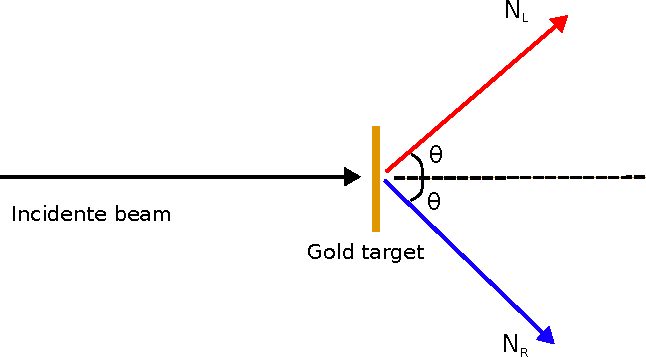
\includegraphics[width = 0.45\textwidth]{ExperimentalSetup/MottScattering.pdf}
\caption{Scheme of the Mott scattering, the polarization is orthogonal to the plane,  $ \vec{n} = \frac{\vec{k} \times \vec{k'}}{|\vec{k} \times \vec{k'}|}$. The red and blue arrows represent two scattering events with the same $\theta$, but opposite $\vec{n}$}
\label{fig:MottScatt}
\end{figure}

The cross section can be modeled highlighting the dependencies on the polarization $\vec{P}$:

\begin{equation} \label{eq:MottCross}
\dfrac{\partial\sigma(\theta)}{\partial \Omega} = I(\theta) [1 + S(\theta) \vec{P} \cdot \vec{n} ]
\end{equation}

In the equation above, the cross section is divided in two terms: $I(\theta)$ represents the term that does not depend on the polarization, while the second term contains the dependence on the polarization, through is the Sherman function $S(\theta)$; also called the asymmetry function \cite{MottElectron}. The unit vector $\vec{n}$ is normal to the scattering plane, and it is defined as:

\begin{align*}
\vec{n} = \dfrac{k \times k'}{|k \times k'|}
\end{align*}

Where $k$ and $k'$ are the wave vectors associated with the incident and scattered electrons. The direction of $\vec{n}$ is parallel to the angular momentum $L$, and depends on whether scattering is to the left or to the right.
Let's suppose our initial beam has a polarization $P$, that can also be expressed as:

\begin{align*}
P = \frac{N_{\uparrow} - N_{\downarrow}}{N_{\uparrow} + N_{\downarrow}}
\end{align*}

Where $N_{\uparrow}$ and $N_{\downarrow}$ are the number of electrons with spin up and spin down. The Mott polarimeter measures the number $N$ of scattered electrons at a fixed angle $\theta$, in the two directions right and left (figure \ref{fig:MottScatt}). Using the equation (\ref{eq:MottCross}), the scattered electrons to the left side $N_{L}$ and to the right side $N_{R}$ are equal to: 

\begin{align*}
N_{L} &= N_{\downarrow}[1 + S(\theta)] + N_{\uparrow}[1 - S(\theta)] \\
N_{R} &= N_{\uparrow}[1 + S(\theta)] + N_{\downarrow}[1 - S(\theta)]
\end{align*}

The asymmetry $A(\theta)$ of the scattered electron between left ($N_{L}$) and right ($N_{R}$) is given by:

\begin{align*}
A(\theta) = \frac{N_{L} - N_{R}}{N_{L} + N_{R}} &= \dfrac{N_{\downarrow}(1 + S(\theta)) + N_{\uparrow}(1 - S(\theta)) - N_{\uparrow}(1 + S(\theta)) - N_{\downarrow}(1 - S(\theta))}{N_{L} + N_{R}} = \\ 
&= \dfrac{(N_{\uparrow} - N_{\downarrow})}{(N_{\uparrow} + N_{\downarrow})}S(\theta) =  P \cdot S(\theta)
\end{align*}

The last step of the equation gives the beam polarization in terms of $A(\theta)$, the asymmetry measured by the Mott polarimeter, and the function $S(\theta)$, the Sherman function. The Mott polarimeter in MAMI, installed after the double solenoid, measures the scattering asymmetry $A(\theta)$ for electrons of $\SI{3.5}{\mega \electronvolt}$ with a thin gold target.  

\section{Experimental Hall Setup} \label{ExperimentalHall}

MAMI experimental halls are named with the capital letter A followed with a number. In A2, for example, photo-nuclear reactions are studied to investigate the fundamental physics at the scale of nuclear dimensions. The experimental hall where the experiment described in this thesis is conducted is the A1 hall. We will describe briefly the main operating detectors that are installed and the details that are interesting for the transverse asymmetry measurement.
In the A1 hall the beam is delivered with energy in a range starting from $\SI{180}{\mega \electronvolt}$ up to $\SI{1.6}{\giga \electronvolt}$. Energy greater than $\SI{855}{\mega \electronvolt}$ are reached with the last acceleration stage HDSM, shown in figure \ref{fig:Accelerator}. Because the electron energy of our experiment is $\SI{570}{\mega \electronvolt}$, the beam passes only through the first acceleration steps, and is extracted from the RTM3 and directly sent to the A1 experimental hall, without going through the HSDM stage. 

\begin{figure}[!ht]
\centering
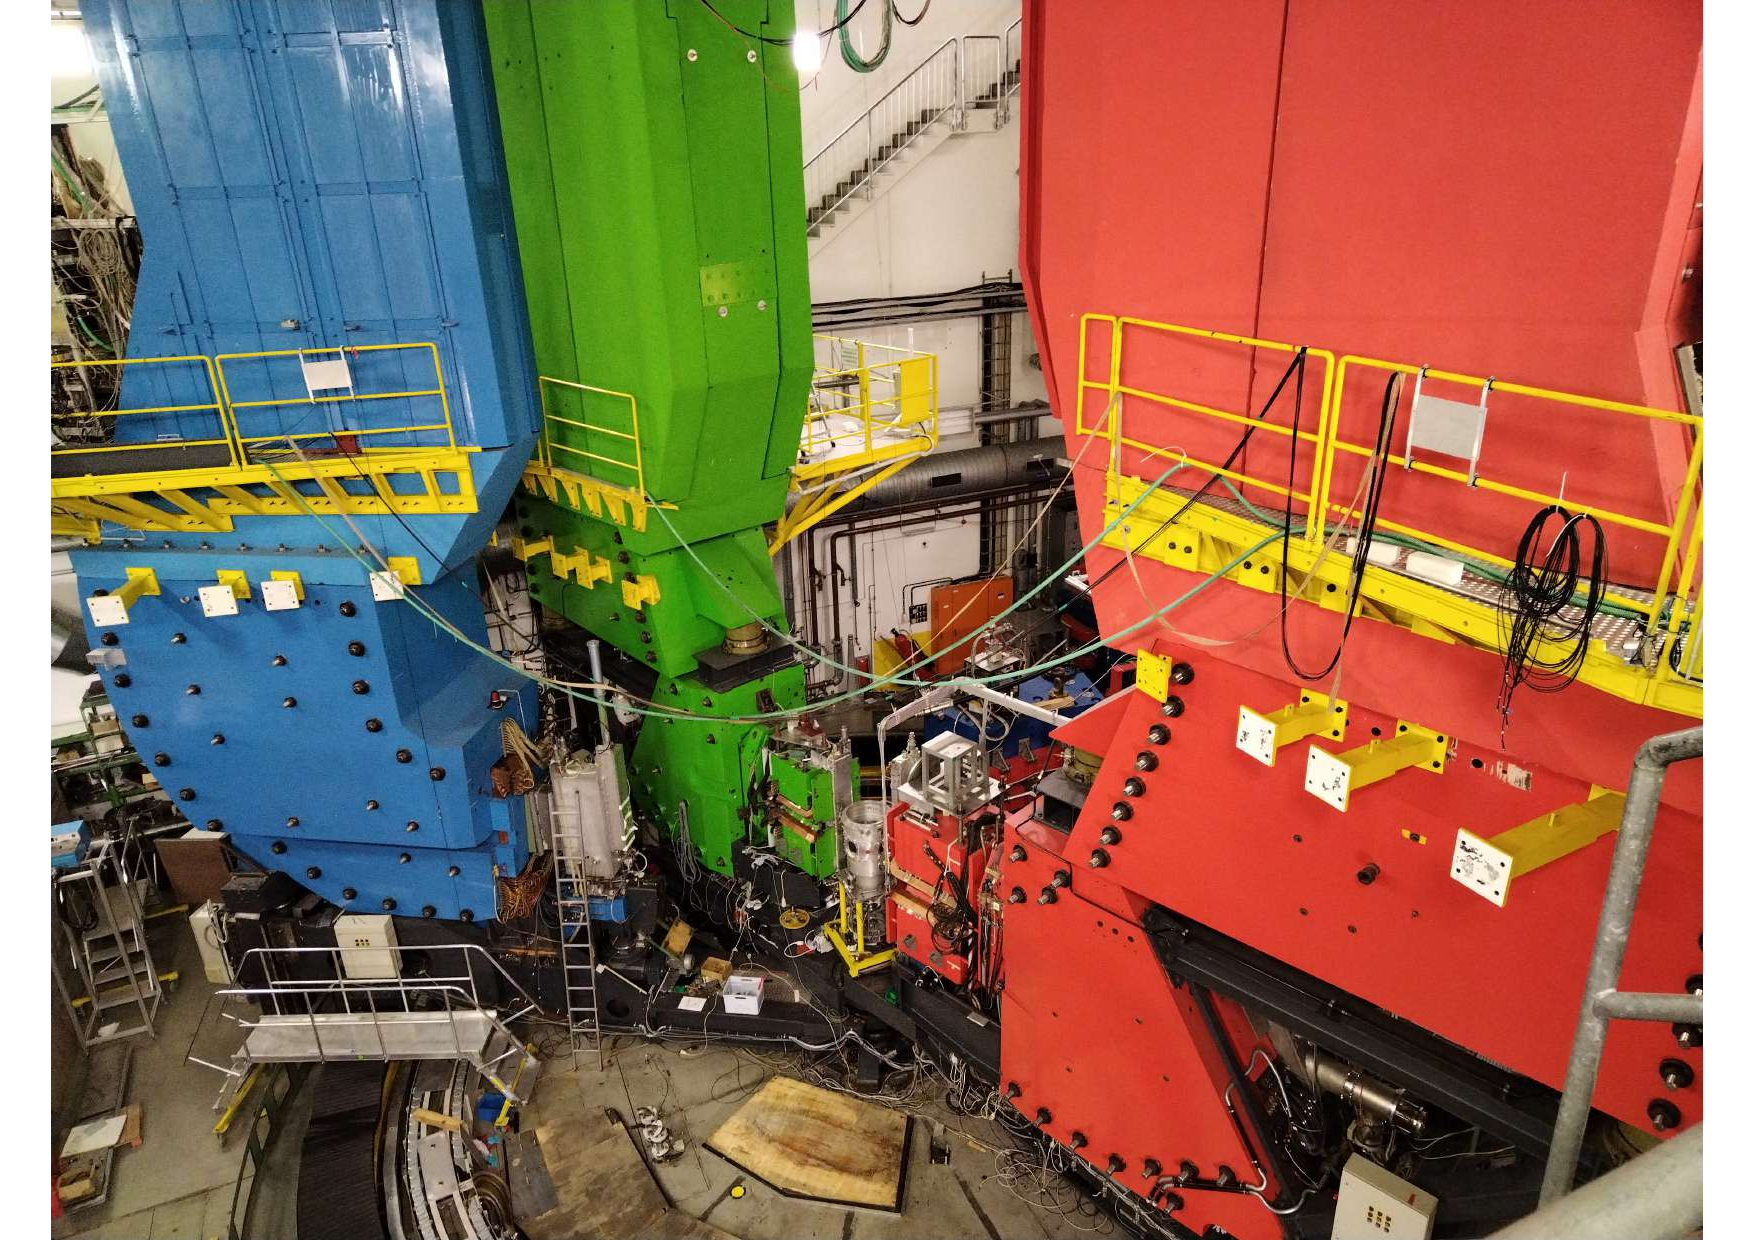
\includegraphics[width = 0.9\textwidth]{figures/twoSpektrometer.pdf}
\caption{Picture of the A1 spectrometers hall, the spectrometers red and blue are used during this experiment. At the center of the picture is possible to observe the scattering chamber.}
\label{fig:TwoSpektr}
\end{figure}

Inside the A1 hall three large magnetic spectrometers are placed on a circular rail-track around the target chamber (figure \ref{fig:TwoSpektr}). They where designed and built in $1993$ to perform high precision measurement of electron scattering in coincidence with other hadron detection, with high resolution in the determination of the particle momenta $\frac{\delta p}{p} < 10^{-4}$. The spectrometers develop vertically with a height of $\SI{15}{\meter}$, and the scattered electrons and the other particles are deflected with respect to the scattering plane with the use of magnetic fields. The figure \ref{fig:TwoDetectors} shows the path of the particles scattered from the target. The spectrometers used for the transverse asymmetry measurement are the red and blue ones. There are multiple reasons why the particle are deflected in the vertical direction, that can be summarized in two points: 

\begin{itemize}
\item reason of space: a horizontal setup would not fit in the dimension of the building; in addition this would not allow to rotate the spectrometers by a variety of angles
\item reduce background and noise: in fact the high beam intensity at MAMI is a source of noise and background events which can be reduced by detecting the scattered particles away from the beam direction.
\end{itemize}    

\begin{SCfigure}[30][!ht]
\centering
\caption{Image of the spectrometers of A1 hall. The spectrometers can be rotated using a system of rail-tracks that are visible at the bottom of the image. The electrons are scattered and then deflected in the vertical direction by the magnetic field (green lines). This picture is taken from behind the target. The target is roughly at the center of the image where the two green lines join. The electron are coming from the opposite direction, with respect to the spectrometers.}\label{fig:TwoDetectors}
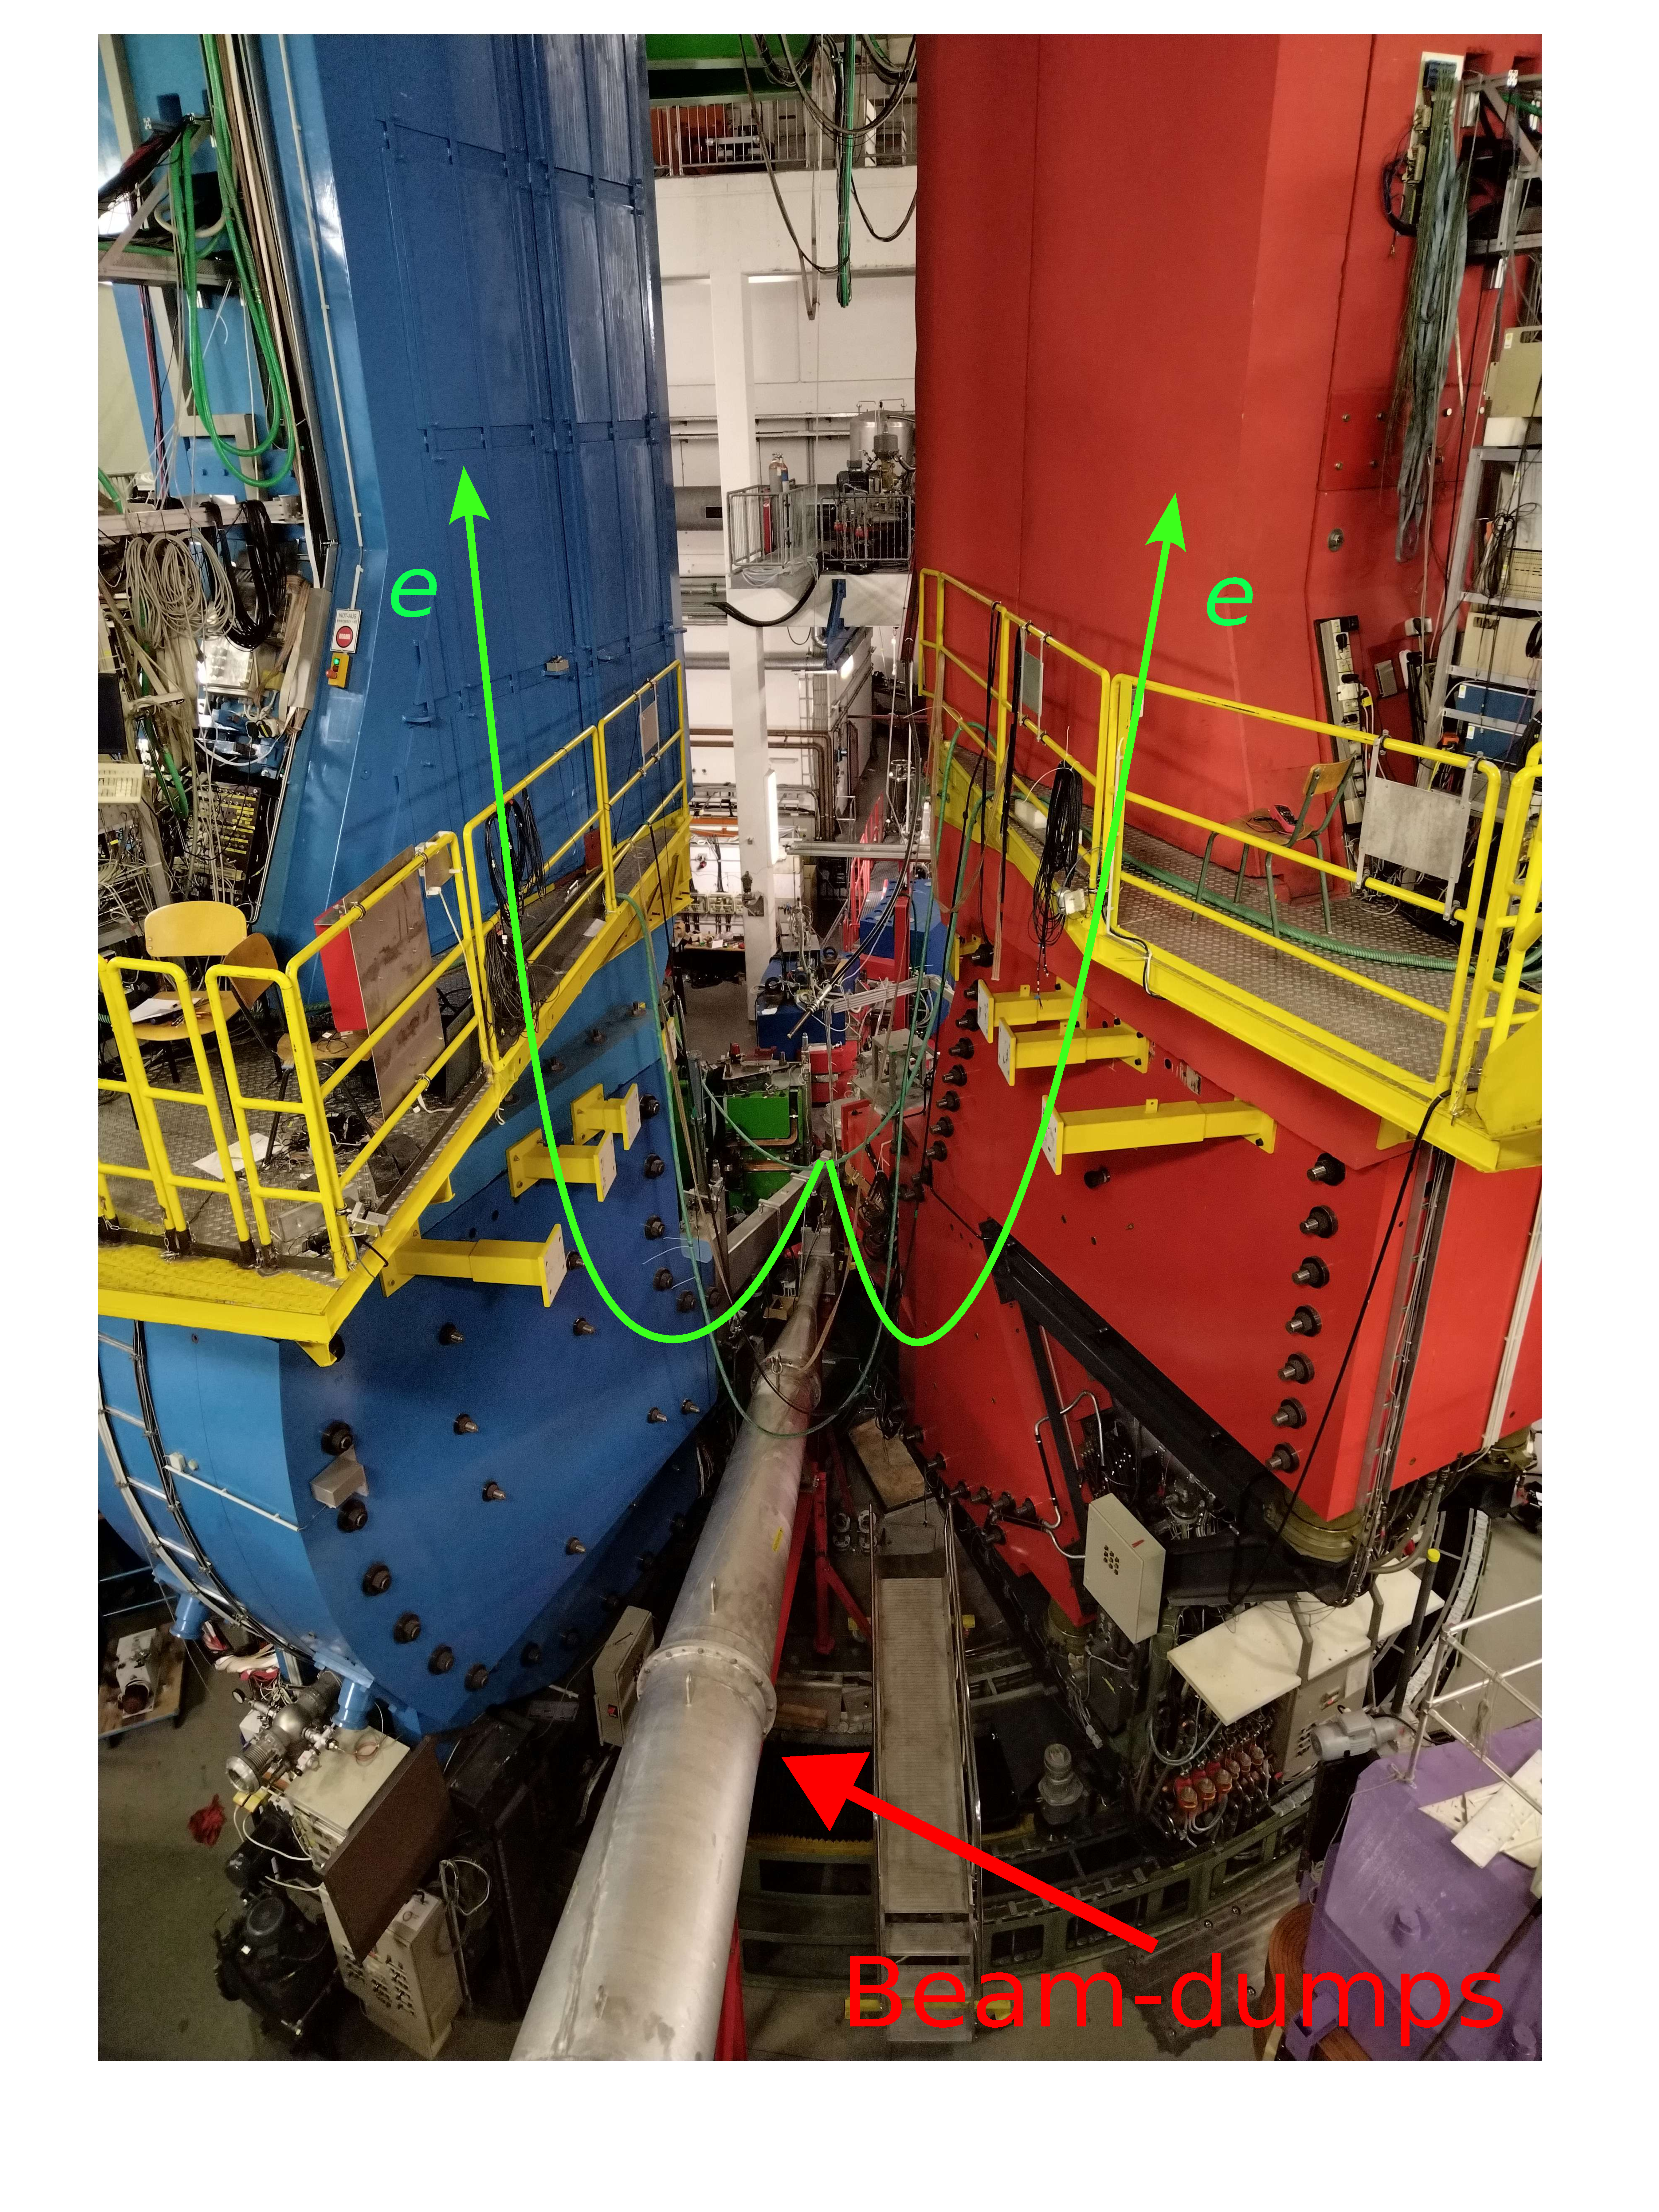
\includegraphics[width = 0.5\textwidth]{ExperimentalSetup/A1_Dietro.pdf}
\end{SCfigure}
  
Once a particle is scattered in the acceptance region of the spectrometers, it is deflected by the magnetic field and passes through the drift chamber, which occupies the first third in height of the spectrometers. 
When the particle is at the height of the platform in the figure \ref{fig:TwoDetectors}, it impinges on a layer of plastic scintillator, and after that a Cherenkov detector  measures the particle speed $v$. In figure \ref{fig:internal} the spectrometer A internal, taken during the installation of detector A, is shown. The determination of both the particle speed $v$ and momenta (drift chamber) allows particle identification.

\begin{SCfigure}[30][!ht]
\centering
\caption{Internal of the spectrometer. This image was taken during the installation of the detector A inside the red spectrometer, that is accessible from the platforms visible in the picture \ref{fig:TwoDetectors}}
\includegraphics[width=0.35\textwidth]{ExperimentalSetup/Detectors/position.pdf}
\label{fig:internal}
\end{SCfigure} 

Despite the possibilities offered by the already existing setup, for the beam time of interest none of these components was used directly in the estimation of $A_{n}$. The reason is due to the high intensity of the beam that is used in the experiment, which is far from the optimal operating conditions of the components, that are suited for rates lower than the ones expected for beam normal single spin measurements (for carbon target $\SI{1}{\mega \hertz}$, while for lead target $\SI{500}{\kilo \hertz}$). The spectrometers are used indirectly, for the alignment of scattered electrons to our detection system.


\section{Detector Description} \label{detectors}
In this section we will describe the electronics and the detectors used to measure the transverse spin asymmetry.
For this experiment we are going to measure the transverse asymmetry at one fixed angle, corresponding to a transferred momentum of $Q = \SI{0.2}{\giga \electronvolt}$. The electrons detection is 
made via two thin blocks of fused-silica that are coupled to PMTs. When a scattered electron hits the fused-silica (refractive index $n = 1.45$) Cherenkov light is emitted. The emitted Cherenkov light can extract one electron in the photocathode, which will be amplified by the PMT dynode structure. This sequence of event triggers the PMT and produce an output signal.

\begin{figure}[!hbtp]
\centering
\subfloat[][\emph{Detector B}]{
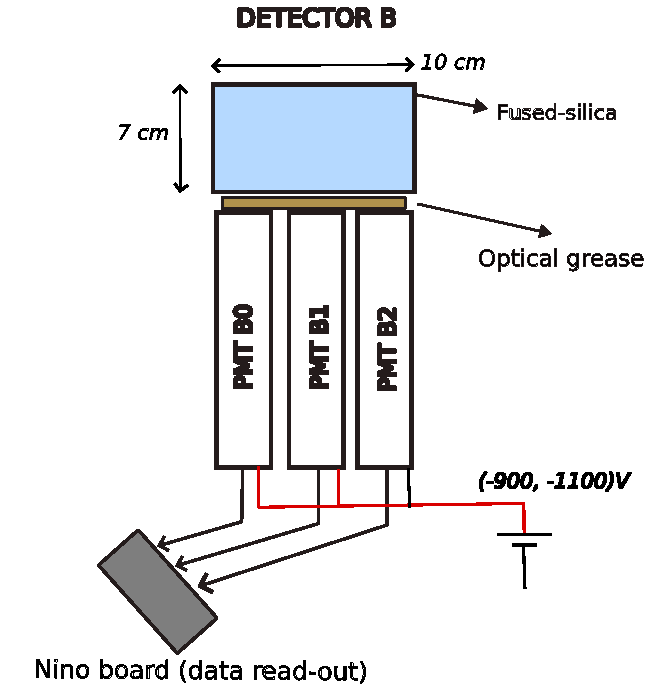
\includegraphics[width = 0.40\textwidth ]{ExperimentalSetup/Detectors/DetectorB.pdf}}
\subfloat[][\emph{Detector A}]{
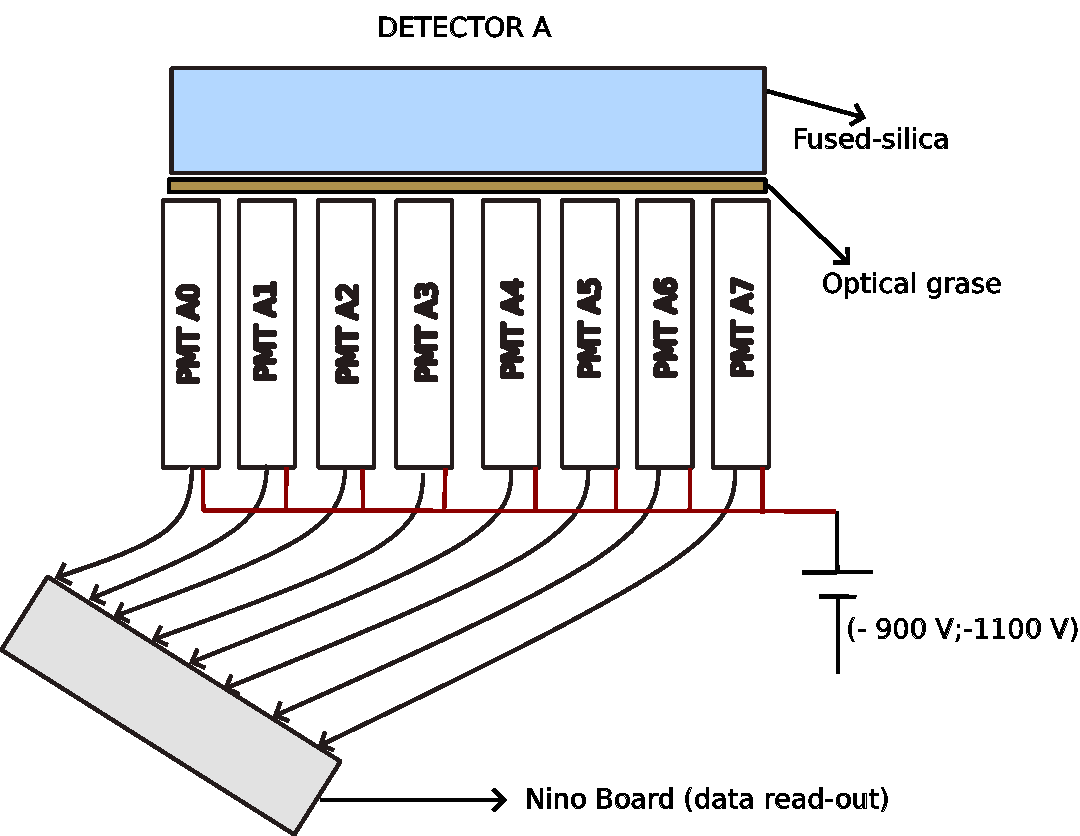
\includegraphics[width = 0.55\textwidth ]{ExperimentalSetup/Detectors/detectorA.pdf}}
\caption{Detector A and B scheme. Each PMT is coupled to the same fused silica bar. The PMTs located at the edges of the fused-silica bars are expected to measure lower rates with respect to the PMTs located near the center. The output signals have negative voltage and are read out by the NINO board.}
\label{fig:DetectorAB}
\end{figure}

In the experiment two detectors are installed and read-out independently. The detector A is placed at an angle of $+\theta$, while detector B is placed at $-\theta$. We expect to measure the same absolute value of the transverse asymmetry, with an opposite sign due to the different orientation. 
The two detector are made by 3 PMTs and 8 PMTs coupled with two blocks of fused-silica, as shown in \ref{fig:DetectorAB}.
These two detectors are placed inside the spectrometers presented in \ref{fig:TwoDetectors}, between the top of the drift-chamber, which occupies the first third in height of the spectrometer, and just below the panel of scintillator. During the experiment, the drift chamber of the spectrometers is turn off, and also the PMTs coupled to the spectrometer scintillators are not powered. The scattered electrons will be detected only via the Cherenkov detectors in figure \ref{fig:DetectorAB}.
As mentioned above, the scattered electron are deflected in the vertical direction by the magnetic field of the spectrometer. It is important to mention the differences between the new and the old electronic setup. In the old electronic setup the output signal of the PMTs was integrated during the time interval of each sub-event, and therefore the single scattered electron could not be counted. The advantage of this method is that the electronics is simpler. However, this old method is affected by a baseline noise and it is not good for the future experiments with lead target, where the expected rates are lower than the rates on carbon.
With the new electronics, the single electrons are counted, and this will enable the future measurements with lead, improving the accuracy. 

\begin{figure}[hbtp]
\centering
\subfloat[][\emph{Detector B}]
	{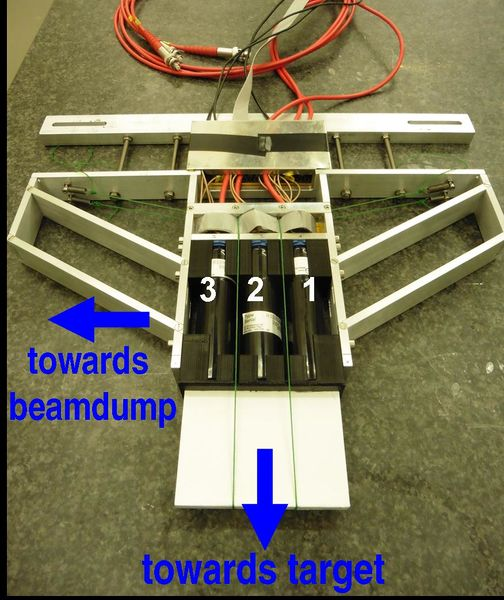
\includegraphics[width = 0.35\textwidth]{figures/504px-Blackfalcon.jpg}} \quad
\subfloat[][\emph{Detector A}]
	{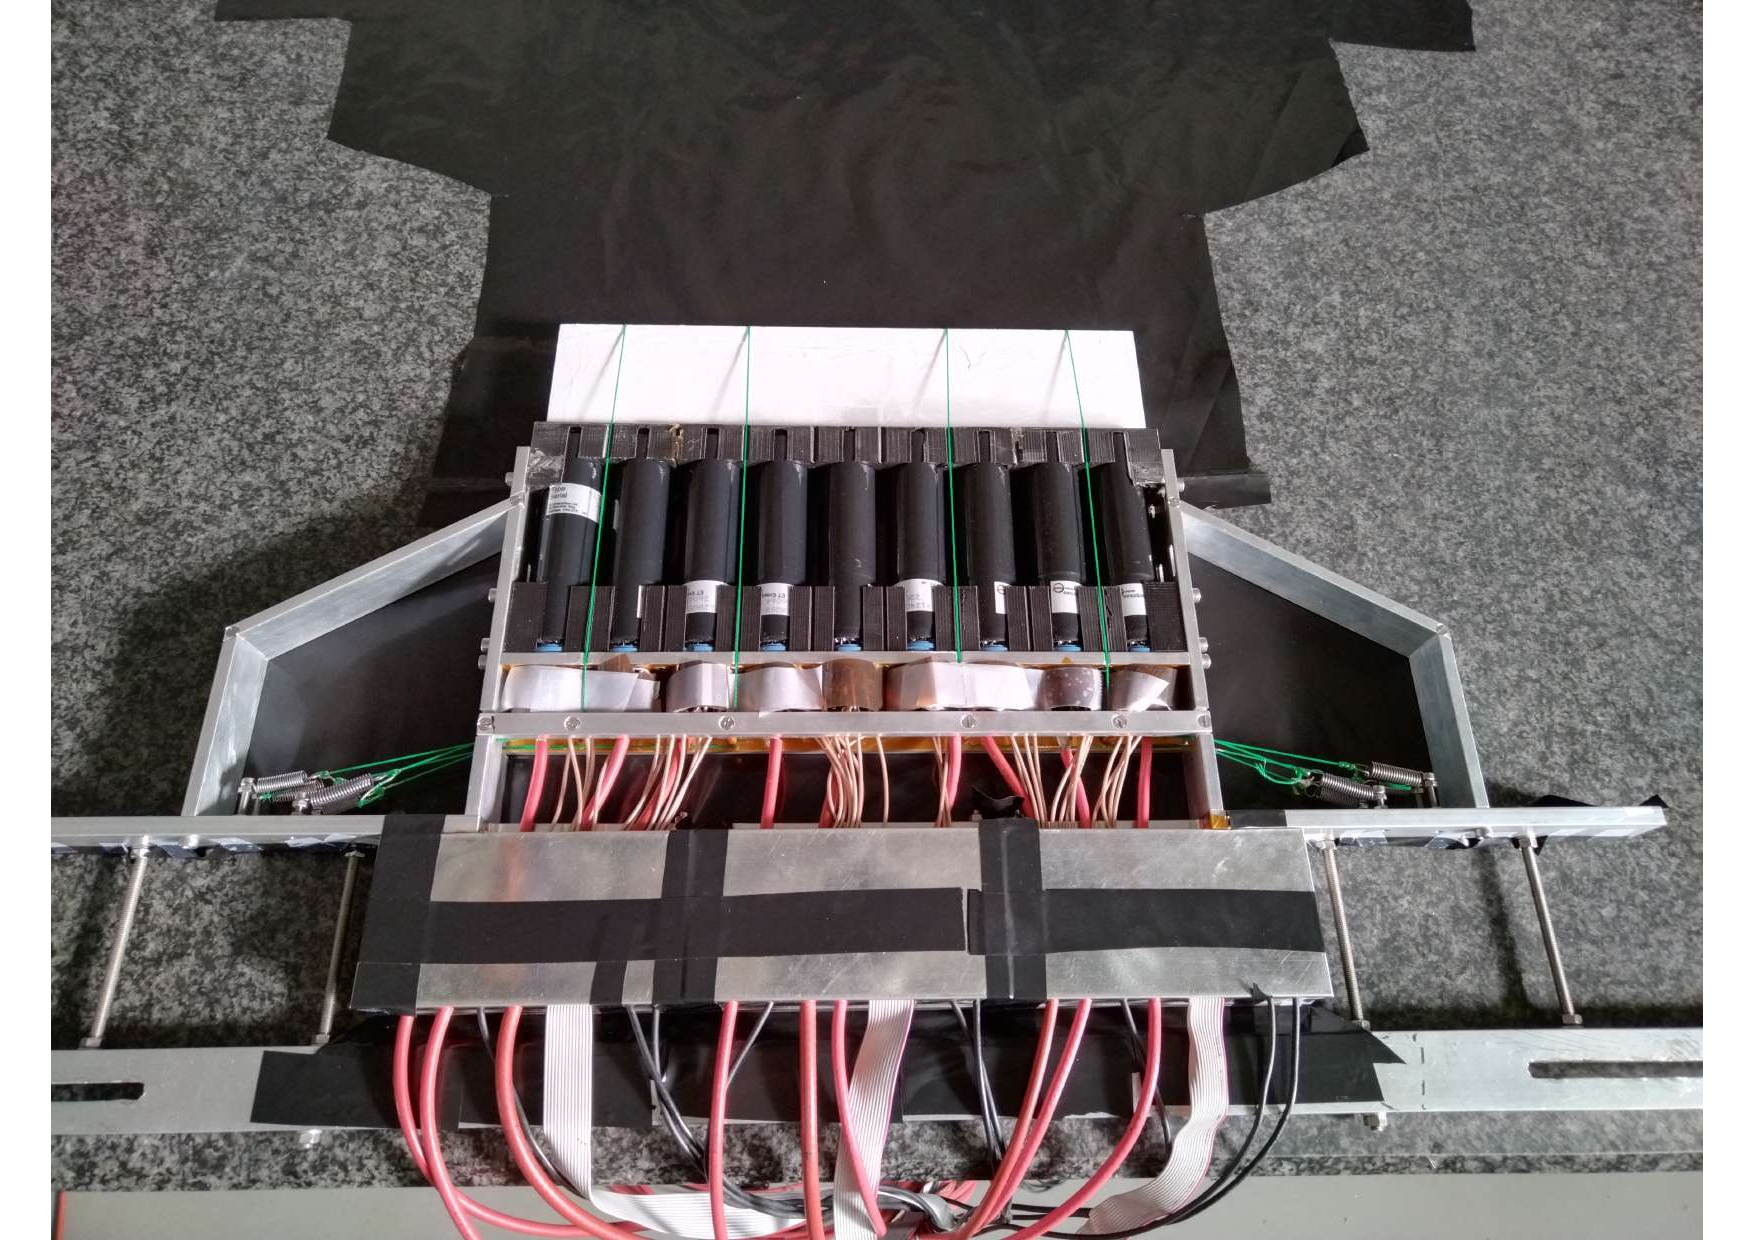
\includegraphics[width = 0.45\textwidth]{figures/IMG_20221110_122246.pdf}} \quad
	\label{fig:Detectors}
\caption{Picture of the two detector taken in the clean room. The white blocks are the fused silica bars that produces the Cherenkov light, the cylinders below are the PMTs, triggered by the passage of the particle. }
\end{figure}

Here we report the characteristic of the two detector that are relevant for the data analysis: 

\begin{itemize}
\item detector B size: $\SI{7}{\centi \meter} \times \SI{10}{\centi \meter} \times \SI{1}{\centi \meter}$
\item detector A size: $\SI{7}{\centi \meter} \times \SI{30}{\centi \meter} \times \SI{1}{\centi \meter}$
\item Number of dynodes of the PMT: 12
\item The Power voltage for the PMT in negative, in the range of ($\SI{-900}{\volt}$, $\SI{-1100}{\volt}$)
\item refraction index $n$ of the fused-silica is $1.45$.
\item maximum gain of $22 \cdot 10^{6}$.
\end{itemize}

The PMTs are coupled to the fused-silica with an optical grease suited for ultraviolet light. The PMTs positioned at the center of the fused-silica bar have an effective area coverage larger than the PMTs at the edge and their rates are expected to be higher compared with the other PMTs. 

\section{Beam Monitors}

In MAMI, several monitors are placed along the beam line to check the beam quality and measure parameters such as current intensity, energy and relative position of the beam. This section summarizes the operating principles of the monitors installed at MAMI. For a complete description, refer to the following paper \cite{M_Dehn} .
The monitors available at MAMI are constituted by resonant cavities. With the resonant cavities it is possible to measure the various quantities, with the underlying physical principle that the passage of charged particles through these cavities excites some electromagnetic resonant modes\footnote{TM mode, where the magnetic field is completely transverse respect to particle momenta} (see figure \ref{fig:CylindricMonit}) which can be detected and analyzed by an analog circuit, and related the beam parameters.

\begin{figure}[!hbtp]
\centering
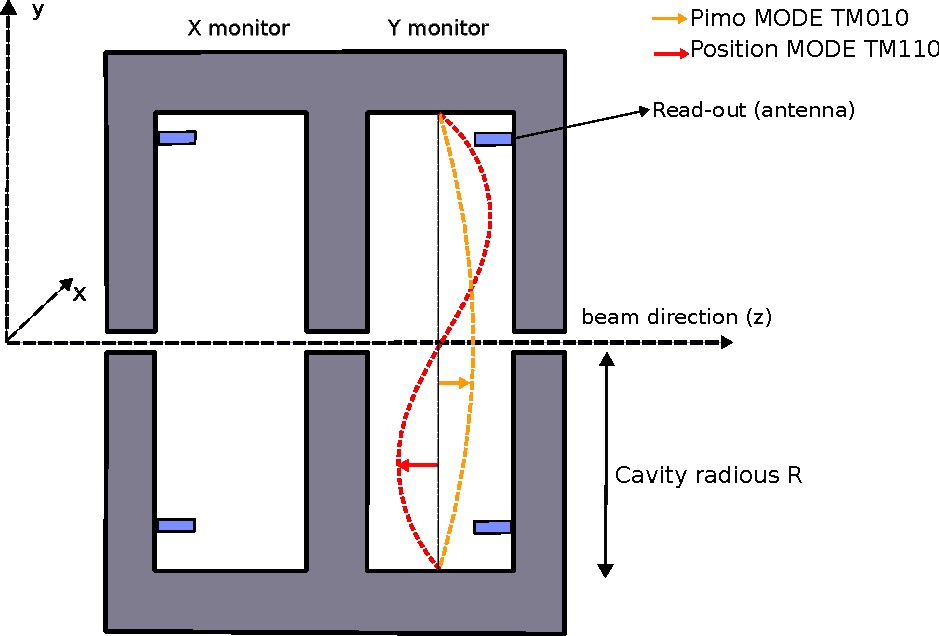
\includegraphics[width = 0.65 \textwidth]{ExperimentalSetup/Monitors.pdf}
\caption{Scheme of the Cylindrical cavities installed at MAMI. In red we have the $TM_{110}$ mode, used to measure the position of the beam, in yellow the $TM_{010}$ mode, to measure the intensity of the beam.}
\label{fig:CylindricMonit}
\end{figure}


Before going into the details, it is necessary to define some quantities that will be used later in the discussion. We define the shunt-impedance $r_{s}$ as:

\begin{equation}
r_{s} = \frac{|V_{\|}|^{2}}{P}
\end{equation}

Where $P$ is the power absorbed by the cavity when a particle excites one of the resonant mode, and $V_{\|}$ is defined as the effective voltage experienced by a charged particle along a straight line, which can be computed as:

\begin{align*}
V_{\|} = \frac{1}{q}  \int_{s_{0}}^{s^{1}} \vec{E}_{s} \cdot  \,d \vec{s}
\end{align*}

The shunt impedance is a measure of the interaction strength between a cavity and a charged particle, and can also be expressed using the $Q$ value of the cavity, the maximum energy stored $W$ and the frequency of resonance $f_{r}$:

\begin{align*}
r_{s} = \dfrac{|V_{\|}|^{2} Q}{2 \pi f_{r} W}
\end{align*}

When the beam travels through the cavity, the particles lose energy that excites the mode. The power $P_{HF}$ extracted from the beam is related to the beam current: 

\begin{equation}
P = i^{2} r_{s}
\end{equation}

Where $i$ is the beam current. An antenna is used to decouple part of the energy from the cavity and send it to a circuit which produces an analog output signal. Indicating with $\kappa$ the coupling constant of the antenna, the previous relation needs to be modified introducing a new factor $ \frac{\kappa}{(1 + \kappa)^2}$. In a cylindrical resonator, the type installed at MAMI, the resonance frequencies of the different oscillation modes are expressed by the formula: 

\begin{align*}
f_{m,n,p} = \frac{c}{2\pi \sqrt{\epsilon_{r} \mu_{r}}} \sqrt{\bigl(\frac{x_{m,n}}{R} \bigl)^{2} + \bigl(\frac{p \pi}{L} \bigl)^{2}}
\end{align*}

The constant in the formula are:

\begin{itemize}
\item $c$ is the light speed.
\item $\epsilon_{r}, \mu_{r}$ are the magnetic and dielectric constant of the material.
\item $x_{m,n}$ it the n-th zero of the m-th Bessel function.
\item $R$ and $L$ are the radius of the cylindrical cavity and his length.
\end{itemize}

This formula can be obtained solving the Maxwell equations with cylindrical boundary condition.
If the frequency of the beam bunch is equal to the resonant frequency $f_{m,n,p}$ of the cavity, a TM mode is excited. At MAMI high quality monitors are installed, with a $Q \simeq 10000$, implying that $\frac{\delta \nu}{\nu} \simeq 10^{-4}$. This means that the frequency of the beam buch must be very close to the frequency of the resonant cavity. At MAMI the frequency used for all the resonators is $\SI{2.449532}{\giga \hertz}$ or a multiple of it. The beam bunch frequency is the same, and it is controlled by the MAMI-master oscillation signal, that is the reference signal for all the MAMI monitors.
Depending on the $TM$ mode excited, we have a different signal in the cavity, so a different signal collected by the antenna. The relevant quantity that is detected is the power $P_{HF}$ absorbed by the antenna, that is proportional to the power loss $P$ of the beam. For the $TM_{010}$ mode, the power absorbed by the antenna is: 

\begin{equation}
P_{HF} = i^{2} r_{010} \frac{\kappa}{(1 + \kappa)^{2}}
\end{equation}

Where $\kappa$ is a coupling constant between the electromagnetic field of the cavity and the antenna.
The power absorbed by the antenna is directly dependent on the beam current. With the beam current in the range of \SI{1}{\nano \ampere} to \SI{100}{\micro \ampere}, the output power ranges from $\SI{}{\pico \watt}$ to $\SI{}{\milli \watt }$. Therefore the signal is processed in close proximity of the installed monitors. In the signal processing, the input signal of the antenna in coupled to the master-oscillation signal, so the output signal is given by the formula:

\begin{equation}
U = \sqrt{P_{HF}} \cos(\phi - \phi_{LO})
\end{equation}

where the phase $\phi$ is the phase of the resonant mode or the phase of the beam bunch, while the phase $\phi_{LO}$ is the phase respect to the master-oscillation signal, and can be adjusted by a phase shifter in the circuit. The output voltage signal can be read out with the oscilloscope or digitalized and saved with other devices. To measure the beam intensity is important to minimize $\phi - \phi_{LO}$ (see figure \ref{fig:PIMO}), to maximize the signal amplitude.

\begin{figure}[!hbtp]
\centering
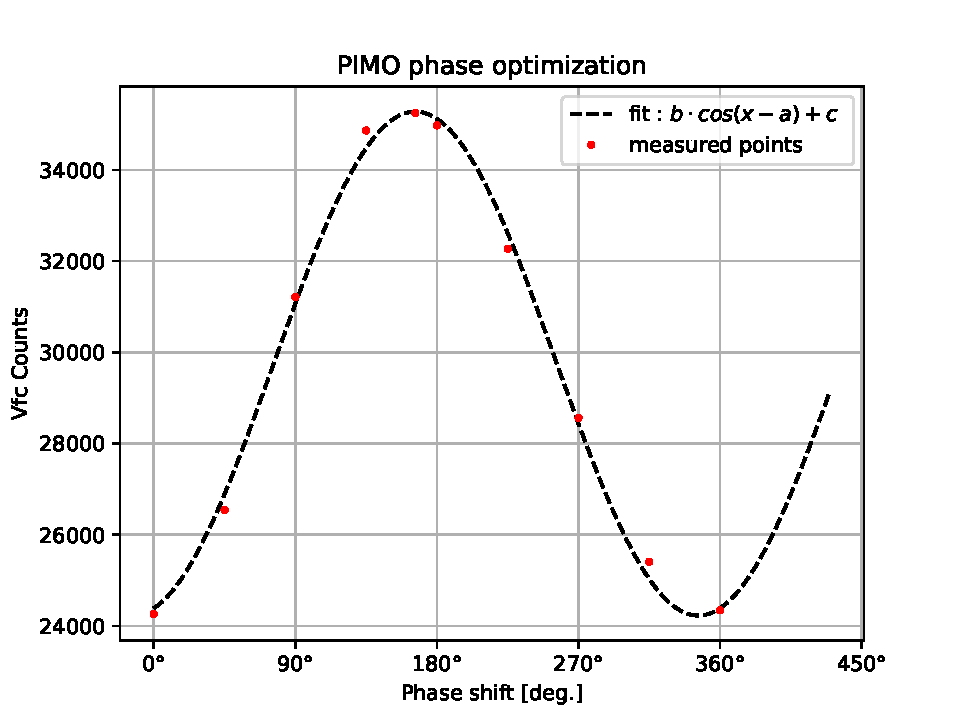
\includegraphics[width = 0.75\textwidth]{ExperimentalSetup/PIMOphase.pdf}
\caption{Plot of the output signal versus phase $\phi$. The phase optimization was done selecting the working point in correspondence of the peak.}
\label{fig:PIMO}
\end{figure}

The measurement of the $x,y$ position follows in principle the same procedure. In this case the $TM_{110}$ is acquired, because for this mode the $r_{shunt}$ is proportional to the beam position on the $x,y$ plane. The power absorbed by the antenna can be written:

\begin{equation}
P_{HF} = i^{2} r_{110} \frac{\kappa}{(1 + \kappa)^{2}} K x^{2}
\end{equation} 
 
The output signal, that is read by our setup, is proportional to the square root of the absorbed power:

\begin{equation}
U = \sqrt{P_{HF}} = constant \, \cdot \, i   \cdot x
\end{equation} 

The beam parameter are obtained by inverting the above formula 

\begin{equation} \label{eq:SignalToVfc}
x \propto \frac{\sqrt{P_{HF}}}{i}
\end{equation}

Where the exact conversion coefficients are not known, and are determined during the calibration phase, at the beginning of the beam time.
To measure the beam energy, a different approach is used. The energy monitor (ENMO) consists of 2 cavities in the RTM3. One is located in the last recirculation pipe, the other one on the part of the beam line, where the acceleration takes place. The two monitors are synchronized to the master oscillation and measure the phase of the bunches of electrons. During their travel from the first cavity to the second cavity, the beam passes through the magnet and does one half turn. If the energy is slightly higher, the radius of the turn will be slightly larger. This means that there is an extra time between the two bunches, that can be measured as a small phase shift in the $\SI{570}{\mega \electronvolt}$ recirculation. From this it is possible to obtain a value for the difference of the actual energy from the nominal energy.

\subsection{Beam stabilization}

The beam stabilization is an essential component of the experiment. The values of $A_{n}$ that we want to measure are in the order of  $10 \, ppm$, so it is important to reduce other contributions that can be related to variations in the beam parameters. The beam stabilization at MAMI is achieved with a control program. The beam monitors constantly measure the beam parameters and the control program receives the measurements from the monitors and calculates consequently the corrections to be performed. 
The beam position in the transverse plane is constantly adjusted by the magnets in the beam line. For the beam current and energy, the control program acts on the laser of the beam source and the klystrons in the three racetrack microtrons described in section \ref{ExperimentalHall}. Two types of stabilization are made by the control program: the first is made to avoid long term drifts by pulling back the beam back to nominal conditions every $\simeq \SI{10}{\second}$. Simultaneously, a fast stabilization prevents fast fluctuation, reacting quickly to every disturbance of the beam. 

\section{Electronics}
\subsection{Voltage to Frequency Converter} \label{VFCss} 

Some beam parameters are needed in order to take into account possible effects in the measurement of the transverse asymmetry. The relevant data are the position in the $(x,y)$ plane, the incident angles on the target, the current and energy of the beam. All this values are collected using the existing monitors. To collect the data from the monitors, single and multichannel, synchronous voltage-to-frequency converters (AD7742) are used. This devices contain an analog modulator that is able to convert the input voltage into an output pulse train, whose frequency is proportional to the input voltage. 

\begin{figure}[htb]
\centering
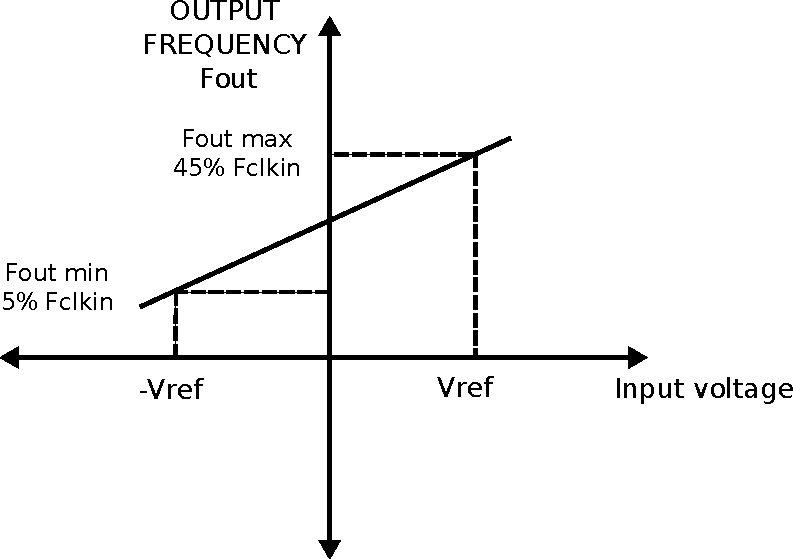
\includegraphics[width=0.5\textwidth]{ExperimentalSetup/Vfc.pdf}
\caption{Frequency versus Voltage}
\label{fig:VoltageToFrequency}
\vspace{10pt}
\end{figure}

The VFCs are powered with an external voltage of $\SI{5}{\volt}$. They measure an input voltage in the range of ($-V_{ref}$, $V_{ref}$). An external clock signal, with a frequency $F_{CLKIN} = \SI{5.88}{\mega \hertz}$ is created externally and synchronous to the gate-length.
The analog input signal is sampled with by a switched capacitor, with a rate that is equal to $F_{CLKIN}$.
The comparator produces a certain number pulses, and the frequency of the output signal is proportional to the input voltage, with $-V_{ref}$ equal to $5 \% \cdot f_{CLKIN}$ and $+V_{ref}$ equal to $45 \% \cdot f_{CLKIN}$ \cite{VfcDatasheet} \commento{, where the first correspond to $\SI{0.0}{ \volt}$ in input and the second to $V_{ref}$}(see figure \ref{fig:VoltageToFrequency}). The data are acquired counting the number of pulses from the comparator, which are proportional to the frequency, so we can substitute to $f$ the number of pulses, and we end up with the equation \ref{eq:Vfc}

\begin{equation} \label{eq:Vfc}
V_{in} =  V_{ref}[2 \cdot \dfrac{N_{pulses} - 5 \% N_{CLKIN}}{40 \% N_{CLKN}} - 1]
\end{equation}

\subsection{Master Board}

The VFCs described in the previous section are measuring the beam parameters along the beam line. A figure of the beam line is in section \ref{XYpos}, where the various position of the monitors is shown.
The data collected by the VFCs are firstly acquired by the master board, in figure \ref{fig:MasterBoard}, and then sent to the A1 computer, which will produce the data package. The VFCs are synchronized by the master board clock, with a frequency of \SI{5.88}{\mega \hertz}. This is also the reference frequency for the VFCs output signal. 

\begin{figure}[hbtp]
\centering
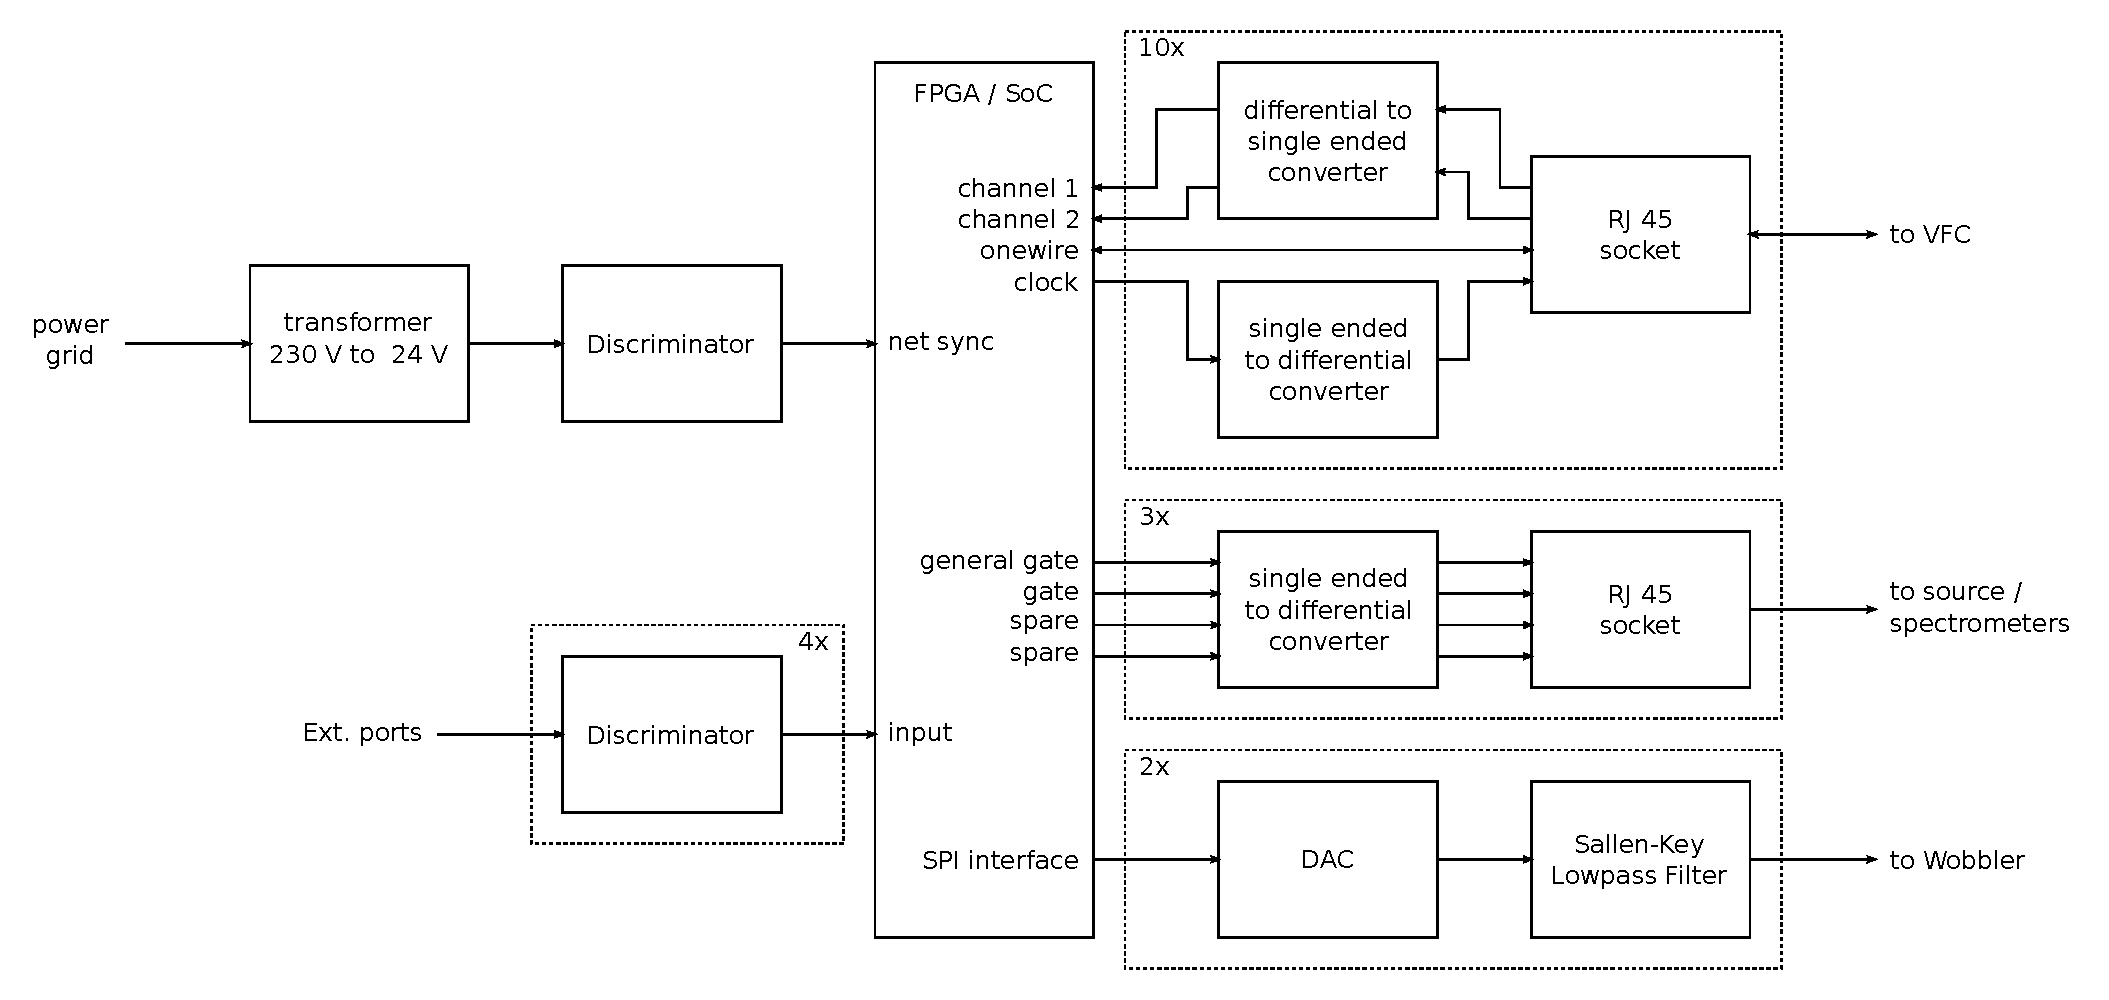
\includegraphics[width = \textwidth]{ExperimentalSetup/masterboard.pdf}
\caption{Scheme of the master-board, the device that coordinates all the electronics for the experiments, and send the data to the computer in the control room.}
\label{fig:MasterBoard}
\end{figure}

The \textit{onewire} is a special bus which will be used in future for temperature measurement in the VFC, to check if there are temperature drift and effects on the outputs signals. The master board sends also the gate length signal to the MAMI source, where the polarized beam is generated, and to the detectors, needed to communicate and synchronize the sub-events. 
For the experiment with the lead target, the master board will also control one of the magnets (\textit{wobbler 16}, in figure \ref{fig:BeamLine}). With the lead target, the beam position must be constantly changed so that the beam hitting point on the target is varies continuously, to avoid melting. The master board is synchronized to the power grid, is order to reduce possible systematics effect connected to the $\SI{50}{\hertz}$ frequency, as discussed in section \ref{FirstDescription}.

\subsection{Nino Board} \label{NINO}

The NINO board shown in figure \ref{fig:NinoBoard} is our data acquisition system for the PMT counts (see paper \cite{1352067}). It is made by $32$ analog input channels and it is powered with $\pm \SI{5}{\volt}$.
Each input channel receives a differential signal from the detector, and has an attenuation circuit that reduces the amplitude of the input signal. After passing the attenuator, the signal is sent to the input stage of the NINO chip, a current-to-voltage converter, that produces an output signal whose pulse-width is proportional to the total charge of the input signal.

\commento{
\begin{figure}[hbtp]
\centering
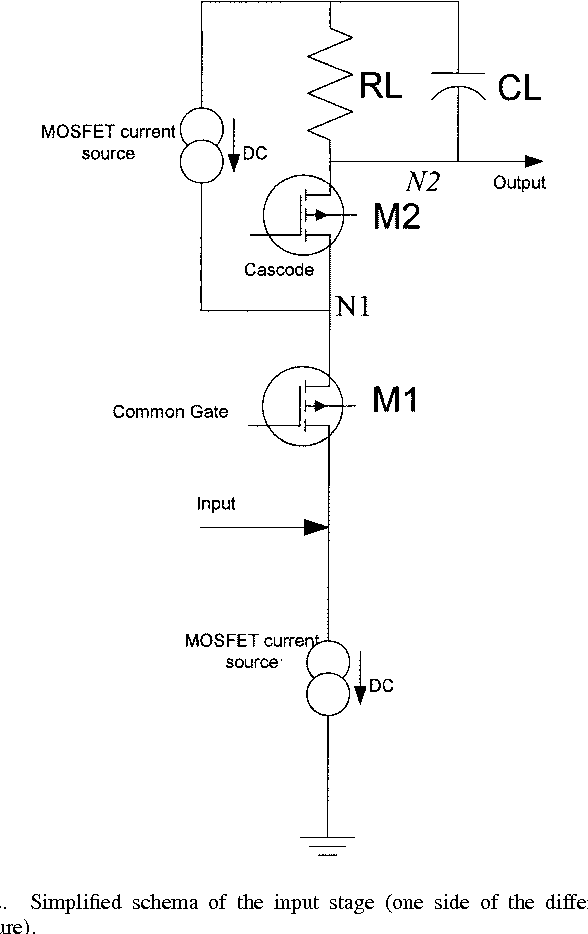
\includegraphics[width = 0.3\textwidth]{ExperimentalSetup/InputStage.png}
\caption{Input stage of the NINO chip. The input signal coming from the detector passes an attenuation circuit, and then are sent to the input stage, in this figure. The output, at node N2, is connected to the discriminator and an amplification stage.}
\label{fig:InputStage}
\end{figure}}

After passing the input stage, the signal goes through a block of 4 cascaded operational amplifiers that act as a discriminator with a programmable threshold. The NINO chip can handle signals coming from $8$ different channels and there are 4 NINO chips on each NINO board. 

\begin{figure}[!ht]
\centering
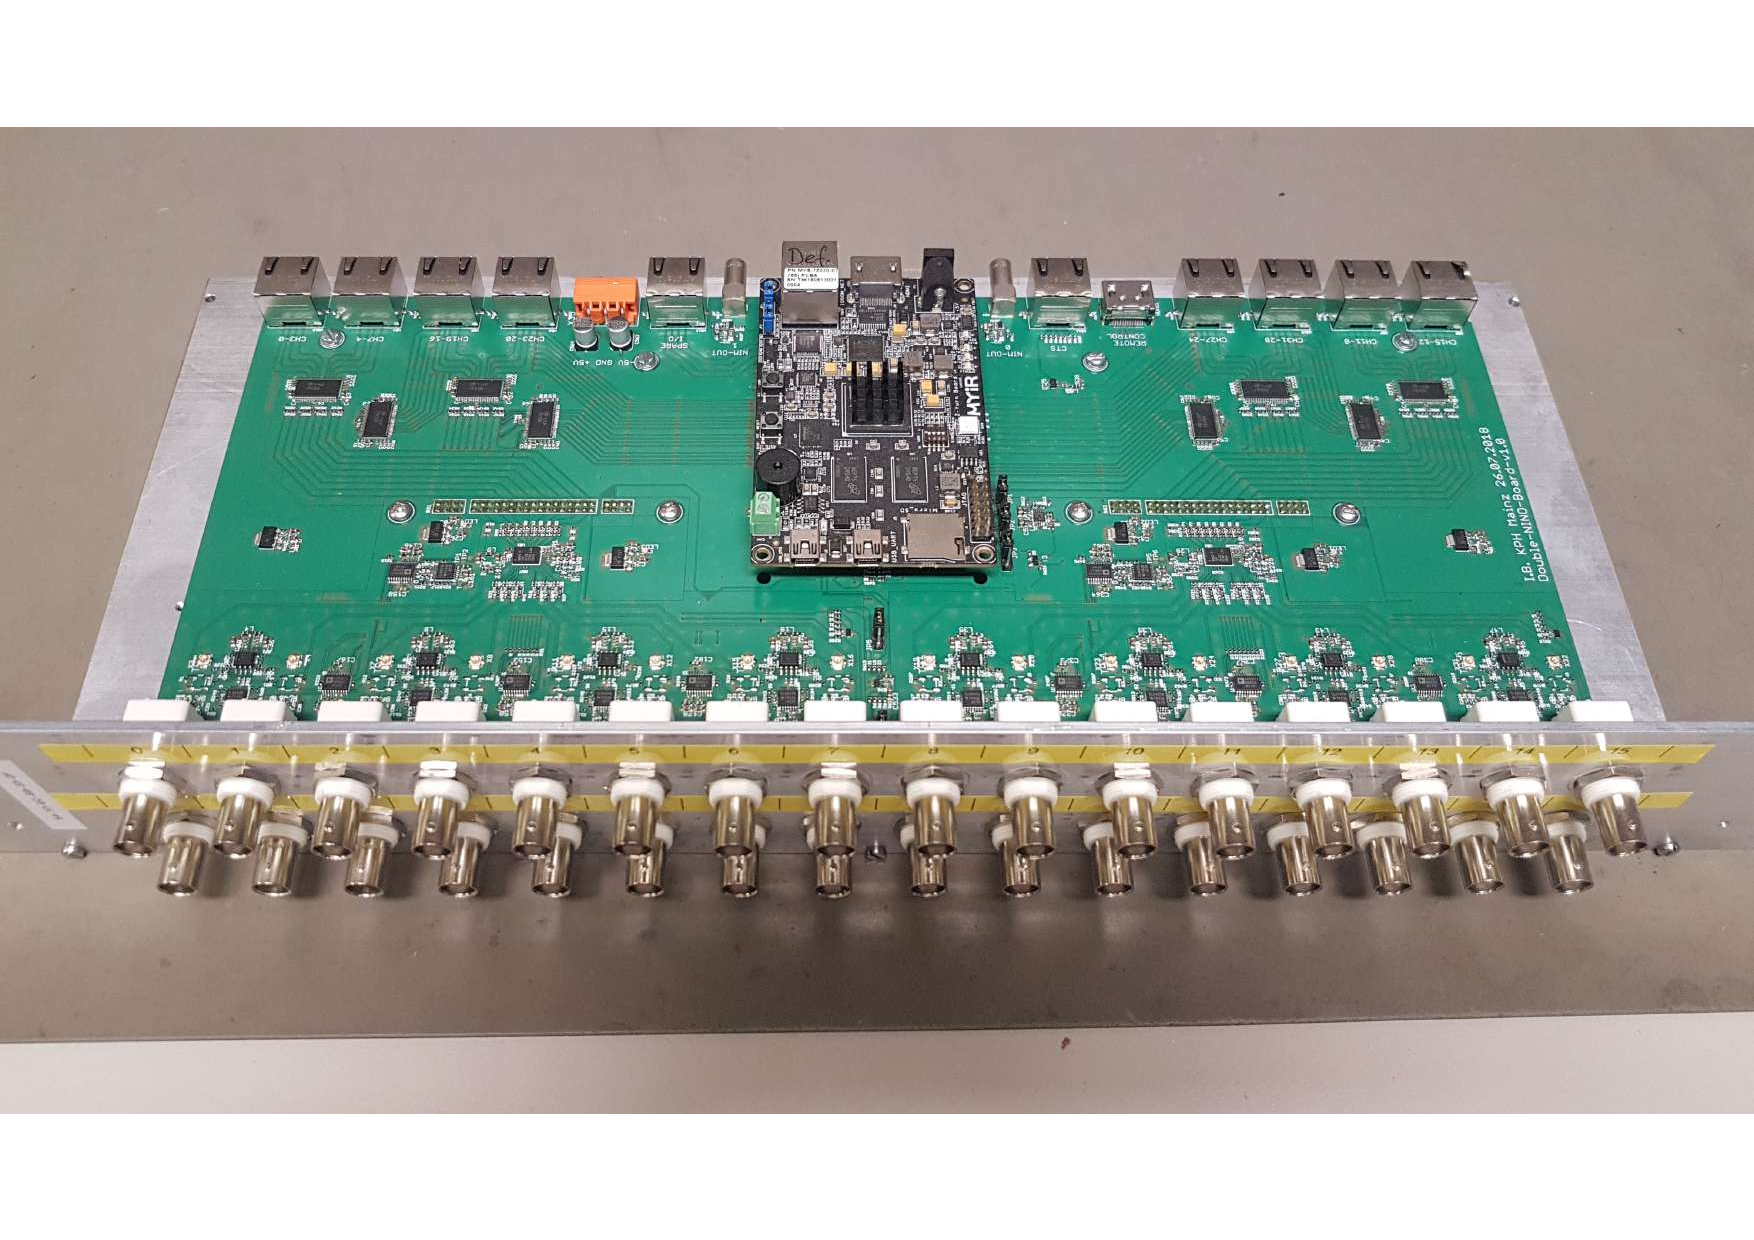
\includegraphics[width = 0.6\textwidth]{ExperimentalSetup/NINO.pdf}
\caption{Nino Board, The input channels are at the bottom of the figure.}
\label{fig:NinoBoard}
\end{figure}
\newpage
The signal that arrives to the discriminator is proportional to the input charge of the signal coming from the detector, so in the end the NINO board is sensitive to the input charge. The discriminator threshold can be set in the range of (\SI{10}{\pico \coulomb}, \SI{100}{\pico \coulomb}). 
The output signal after the discriminator and the amplification block is a LVDS (low voltage differential signaling) with a fixed shape, and a width that is proportional to the input charge. Regarding the data acquisition system, two values are import to control the discriminator threshold and the attenuator, and are named \textit{Thr} and \textit{Att}, respectively. The NINO chip is designed in such a way that the \textit{Thr} value is shared by 4 adjacent channels. On the contrary each channel has is own value of \textit{Att}. Acting simultaneously on \textit{Thr} and \textit{Att} is possible to define a global threshold for each channel, individually.
These two parameters are set in the DAQ program, using 12 bit DACs, corresponding to an interval of $(0 ; 4095)$. \textit{Thr} selects the threshold of the discriminator. The \textit{Att} value controls the input voltage of attenuator: the higher is the value of \textit{Att}, the lower is the attenuation of the signal.
Two Nino board are used in the experiment, one for detector A and one for detector B. For the experiment discussed in this thesis, we will use only 8 channels for detector A and 3 channels for detector B, since this is the number of the input signals coming from the two detectors. For the future experiments more channels will be used, splitting the analog input signal in 4, and sending it to 4 different input channel of the board. This is useful because changing individually the attenuation value, we can define 4 different thresholds for the same signal and compare different values of threshold, to study how the noise affects the measurement, finding the best compromise between signal to noise ratio. The \textit{Thr} and \textit{Att} selection is explained in chapter \ref{analysis}.




\chapter{Detectors Test, alignment and calibrations.} \label{analysis}
\commento{
\begin{outline}[enumerate]
\1 development of the analysis program.
\1 testing the analysis program with montecarlo data.
\1 Test of the detectors in the Lab.
\1 Beam line description.
\1 Data Analysis
	\2 thresholds scan
	\2 Rates on $Pb^{208}$.
	\2 Beam related asymmetry correction.
	\2 $C^{12}$ Asymmetry.
\end{outline}}

\paragraph{Introduction}
In this chapter we discuss the electronic test that have been carried out in the laboratory, and the calibrations that need to be done
in order to calculate, from the raw data, the final data ready for the analysis.
The test in the lab consist in checking that the photo-multipliers are working and that the electronics that take care of acquiring the data do not have any errors.
For the calibrations, since several beam parameters are needed for the analysis, it's important to obtain the correct scaling factor to convert the Raw Data collected by the \textit{VFC}s to data with the right physical units. The important quantities are the $X,Y$ impact point coordinates of the beam,the energy $E$, the beam current $I$ and the scattering angles $\theta_{x}$ and $\theta_{y}$.

\section{Data tree implementation}

Referring to the next picture, we now discuss briefly the structure of the data that is implemented in the analysis program, this is important to clarify how data analysis will be developed:

\begin{figure}[hbtp]
\centering
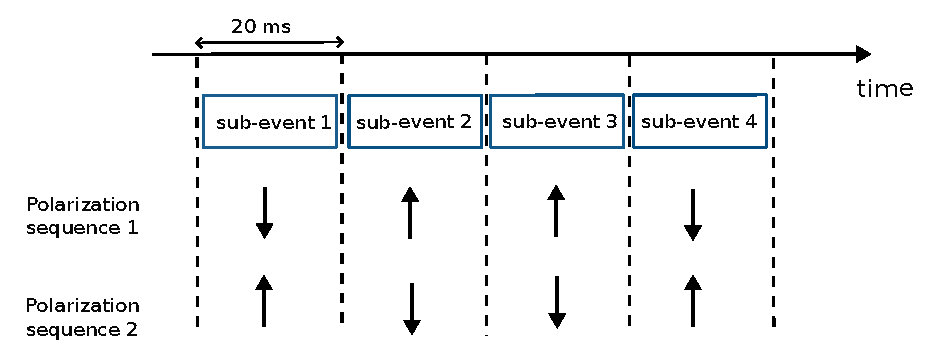
\includegraphics[width = 0.75\textwidth]{ExperimentalSetup/EventStructure.pdf}
\caption{}
\end{figure}

The base class that is implemented in the analysis program is the \textit{Event} class. As we mention above in \ref{FirstDescription}, we do not intend to keep track of the single scattered electron, instead we analyze time series of $\SI{80}{\milli \second}$, in which we simply count all the electrons detected in this time interval. The work-flow of the analysis program is load the binary file collected during the beam time, parsing  one event at a time and processing the raw-data from the beam monitors and the detectors. During the execution of the program data files in \textit{.txt} are generated and filled with the processed data ready. The output data-file can be analyzed with any software package, such as root or python, to get the value of the asymmetry $A_{n}$. 
The picture shows that every event is divided into $4$ sub-events. For each different sub-event a precise state of the polarization is defined, 
$+1$ for $S = \uparrow$ and $-1$ for $S = \downarrow$. Every sub-event is $\SI{20}{\milli \second}$ long; during this time interval master-board receives all the data coming from the monitors and the detectors and sent them to the data-acquisition program (DAQ) that produces the binary-files, which are the input of the main analy\begin{figure}[hbtp]

\centering
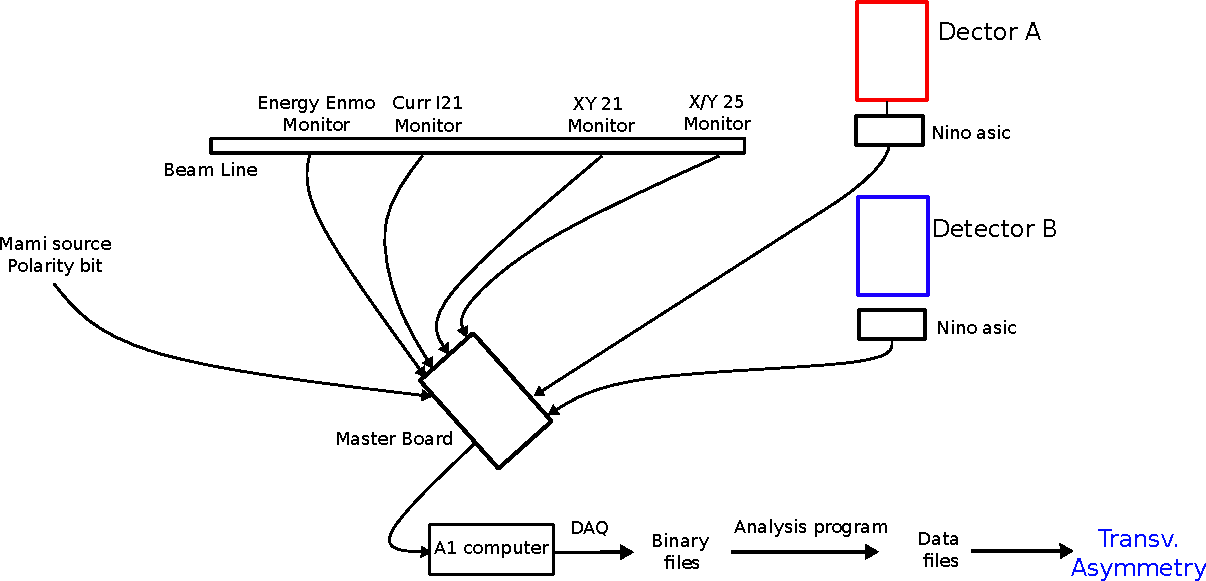
\includegraphics[width = 0.75\textwidth]{Analysis/Electronic_scheme.pdf}
\caption{Scheme of the data flow.}
\end{figure}
sis program.

 It is important to note that for each sub-event, a single measurement is acquired from the beam monitors, which is intended as a time average of the various signals on the 20 milliseconds of sub-event duration. The sampling rate is then equal to $\SI{50}{\hertz}$.

This structure of the data is quite specific for particle physics experiment. The main reason for this setup is connected with the need to avoid as much as possible that the variations of intensity, position and energy of the beams induce an effect that add to $A_{n}$. Considering only small time series, it is assumed that the beam is quite stable, in order to reduce undesired effects.
Nevertheless, the contribution of these effects, which are indicated for brevity as false asymmetries, is considered in the final model.
Several values are saved with the number of scattered electrons, for each event. Here we will present briefly all the various quantities that are saved, and the general structure of the data tree:

\begin{figure}[hbtp]
\centering
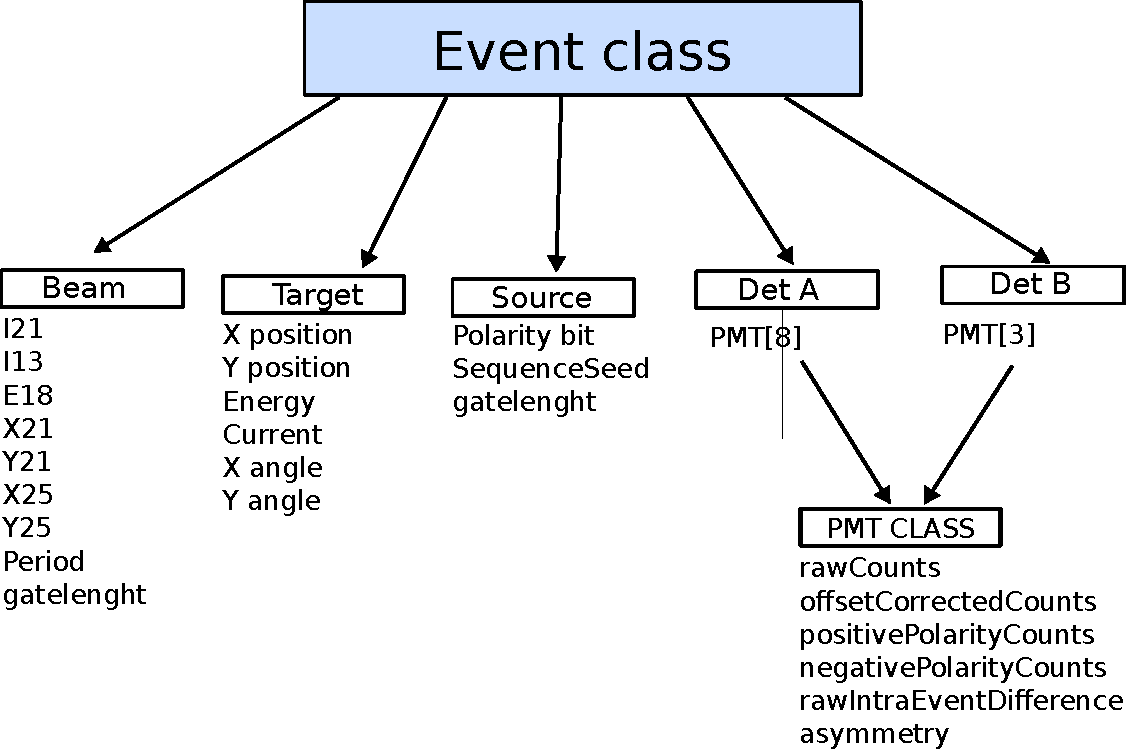
\includegraphics[width = 0.8\textwidth]{Analysis/EventClass.pdf}
\caption{Scheme of the Event class, the structure of the data treen is shown here in a simplified version, for the complete reference see appendix.}
\end{figure}

\section{Nino Board characteristics}
In this section we explain briefly simple test that we performed to control that the two detectors are working properly.Before going into detail it is important to describe again the operation of the NINO board, which interfaces directly with detectors.
The Nino board, which digitizes the signal from the PMTS, has two parameters which can be used to select the internal threshold of the discriminator, to cut out the low amplitude signals, that are indicated as threshold and attenuation. The threshold and attenuation values can be adjusted changing the settings of the DAQ program.
For our purpose, we fix the threshold values equal to $600$ for all the detectors. We remind the reader that the values should be in the range ($0,4000$). 
It is desirable to work with the "physical" values, i.e switch from these arbitrary units to the correct value in $\SI{}{\milli \volt}$. The relation between attenuation and threshold it is not linear, the reason is that the NINO board is designed in such a way that collects the input charge coming from the signal. In principle it is even not possible to define a unique value for the threshold in $\SI{}{\milli \volt}$, because signals that produce the same charge can have shape and amplitude different from each other. In simple word, from the definition of the current:

\begin{align}
Q = I \, \cdot \, time
\end{align}

Signal with a large time width and a small amplitude can generate the same accumulation of charge respect to narrow signal with high voltage amplitude. Despite this, some data have been acquired by the A1 collaboration, with which it's possible to define a raw conversion function from attenuation units to threshold. The basic idea is to fix th time-length and the shape of signal and vary the amplitude, then we can observe the minimum value of attenuation for which the NINO board collects the input signal. We are aware that for electrons that hit the detectors, the shape of the signal cold different, and are not fixed, however this procedure let us to have at least a first rough estimate of the threshold value.

\begin{figure}[hbtp]
\centering
\subfloat[][\emph{Threshold dependence against attenuation} \label{fig:ThrvsAtt}]{
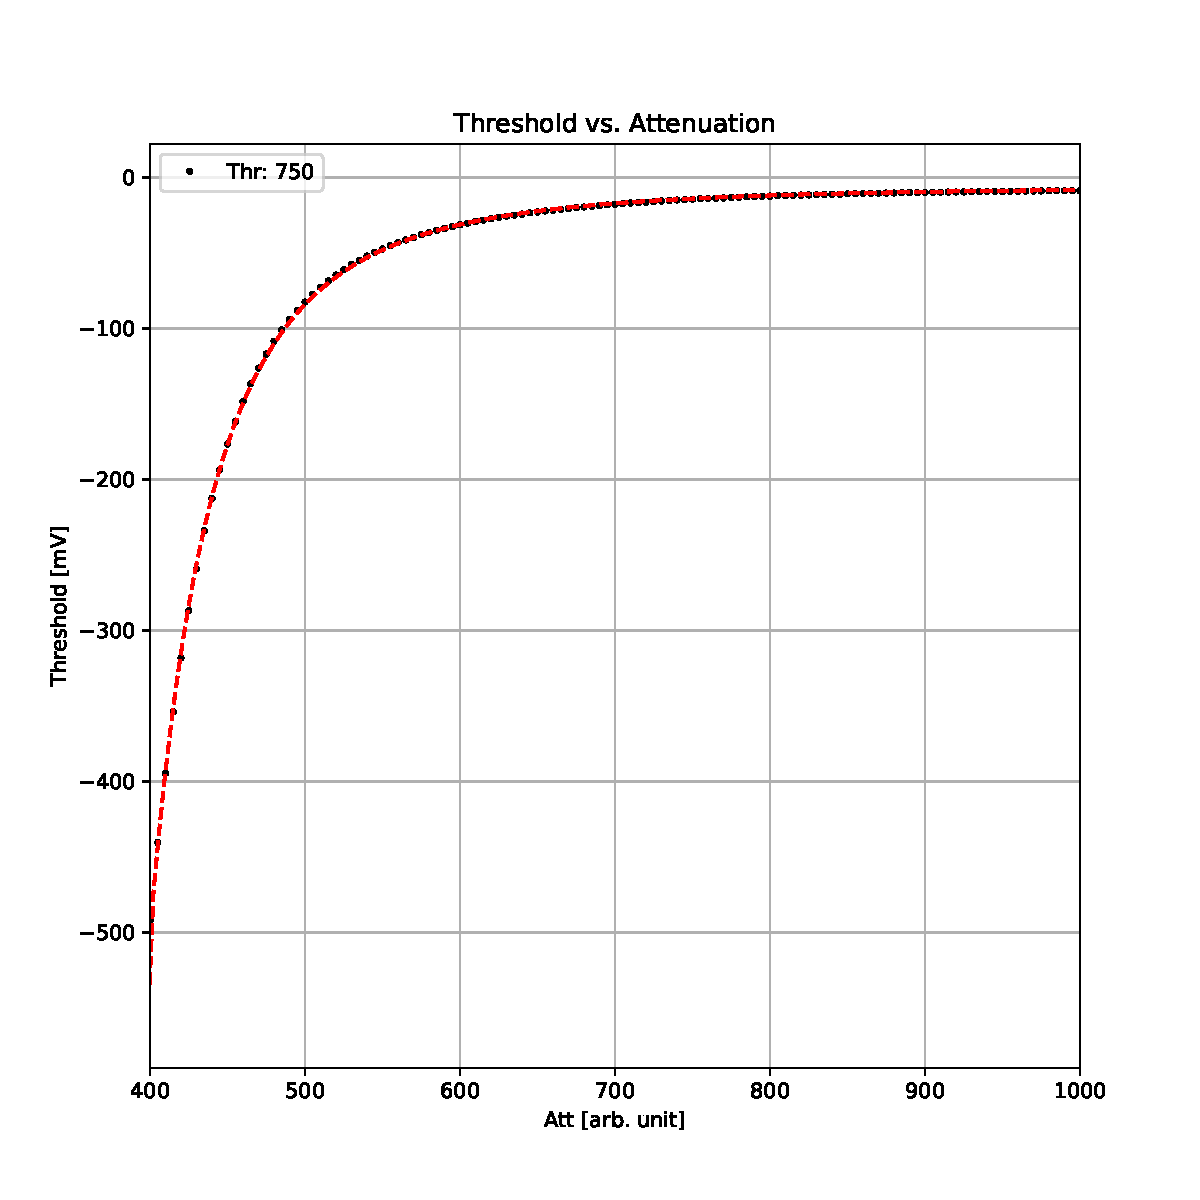
\includegraphics[scale=0.4]{Analysis/Calibrations/ThrvsAtt.pdf}}
\end{figure}

The data show represent the values of the amplitude of the input signals (in $\SI{}{\milli \volt}$) versus attenuation, the function used for the conversion is obtained from the fit of the data, the function used is the following: 

\begin{equation}
Threshold = \dfrac{a}{(att - b)^{3}} + c
\end{equation}

The values obtained from the fit are:

\begin{itemize}
\item $a = - 802111053 \, \frac{\SI{}{\milli \volt}}{[arb.unit]}$
\item $b = 382 \, [arb. unit]$
\item $c =  \SI{-6.1}{\milli \volt}$
\end{itemize}

\section{Detectors test}

Before the Beam time, some test with the two detectors were performed, to check that the pmts were still working after some years of inactivity, and that the new electronic was able to count properly the pulses and store the data. For this studies, we didn't have a radioactive sources to employ, so we moved the two detectors in the workshop of the accelerator, and we use the cosmic rays rate as a probe. 

Knowing that the expected number of event for cosmic rays is about $1 \frac{event}{\SI{}{\centi \meter\squared} \SI{}{\second}}$ we can compute the expected values for the number of events. We decided to take 1 minute long acquisition for both the two detectors, this leads to $70$ expected events for detector B  and  $100$ events for detector A.  \smallskip

The first step is to select a good point of work for the threshold. So, fixing the value of the threshold parameter for the NINO board, we took several acquisitions, each of them one minute long, increasing each time the attenuation. We powered the pmts with a negative voltage around $ \SI{-1000}{\volt}$, as suggested in the data-sheets, and covered the cherenkov detector with a shielding blanket, to avoid ambient light simulating a signal.

\begin{figure}[hbtp]
\centering
\subfloat[][\emph{Attenuation scan for Detector B}]{
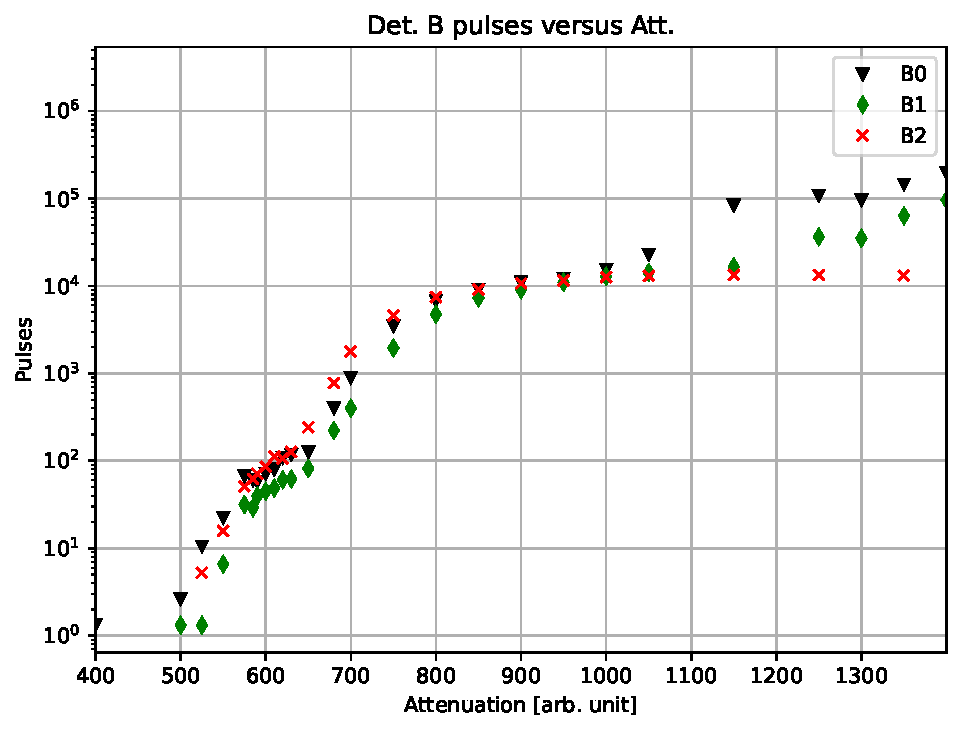
\includegraphics[width = 0.45\textwidth]{Analysis/AttenuationB.pdf}}
\end{figure}

We observed a small knee in the plot, around the zone of 580 − 600 of attenuation, where the number of counts was almost constant, roughly equal to the number of expected events from muons hitting the detector. Then we observe a big edge for attenuation = 1000. Looking at the plot \ref{fig:ThrvsAtt}, we assume that the attenuation values are so high that electronic noise is no longer rejected, in fact the counts grow enormously. The attenuation was set at 600.

The next step was to study the statistical fluctuation of the counts, so we collected 10 acquisitions, each of them 1 min long. The measured values are reported in the table below:

\begin{center}
\begin{tabular}{|c|c|c|c|}
\hline 
Pmt: & 1 & 2 & 3 \\ 
1 & 58 & 60 & 62 \\ 
\hline 
2 & 62 & 55 & 59 \\ 
\hline 
3 & 61 & 59 & 70 \\ 
\hline 
4 & 73 & 66 & 70 \\ 
\hline 
5 & 68 & 66 & 56 \\ 
\hline 
6 & 59 & 52 & 64 \\ 
\hline 
7 & 69 & 74 & 77 \\ 
\hline 
8 & 48 & 49 & 57  \\ 
\hline 
9 & 70 & 54 & 58 \\ 
\hline 
10 & 60 & 61 & 66\\
\hline
\end{tabular} 
\end{center}

This data are interesting to check if the counts are following the theoretical distribution of the events expected for cosmic rays at sea level. If the pmt are working in a good mode, we know that the number of counts should be Poisson-distributed:

\begin{equation}
Pdf(\mu,k) =  \frac{\mu^{k}}{k!} e^{-\mu}
\end{equation}

The variance of the Poisson distribution is equal to the mean of the counts, and we expect the same behaviour also for the sample mean and the sample variance:

\begin{align*}
\begin{split}
\mu_{1} = 62.8	\qquad \sigma^{2}_{1} = 54.40 \qquad r_{12} = 0.66\\
\mu_{2} = 59.6	\qquad \sigma^{2}_{2} = 57.15 \qquad r_{23} = 0.65\\
\mu_{3} = 63.9	\qquad \sigma^{2}_{3} = 46.98 \qquad r_{13} = 0.35 \\
\end{split}
\end{align*}

We report also the correlation $r_{xy}$ between the pmt. The result are fine: we are able to see a positive correlation between adjacent pmt, and as expected the correlation is lower in the case of the more distant. This is explained by the lower probability that the photons of Cherenkov radiation light up at the same time pmts that are far away from each other.
We can test that the data follow a Poisson distribution using the well-known Gosset test, defined as:

\begin{equation}
\chi^{2}_{n-1} = \sum_{i = 1}^{n} \dfrac{(Oss_{i} - Att_{i})}{Att_{i}}
\end{equation}

We report the result obtained with the data for detector B, the test shows that there is good agreement with the hypothesis that the count are Poisson-distributed.

\begingroup
\setlength{\tabcolsep}{8pt} % Default value: 6pt
\renewcommand{\arraystretch}{1.2} % Default value: 1
\begin{center}
\begin{tabular}{|c|c|c|c|}
\hline 
Pmt: & 1 & 2 & 3 \\ 
\hline
$\chi^{2}_{9}$ & 8.52 & 8.45 & 6.37 \\ 
\hline
\end{tabular} 
\end{center}
\endgroup

To convince oneself that the pmt are actually measuring signals given by the passage of cosmic rays, and not only noise, we placed one pmt in coincidence with the others. If we are able to observe positive correlation between the counts, we conclude that the signal comes from the same event.

\begin{center}
\begin{tabular}{|c|c|c|c|c|}
\hline 
pmt & 0 & 1 & 2 & 4 (in coincidence) \\ 
\hline 
1 & 63 & 57 & 72 & 28 \\ 
\hline 
2 & 55 & 51 & 64 & 18 \\ 
\hline 
3 & 62 & 53 & 75 & 27 \\ 
\hline 
4 & 71 & 62 & 75 & 33 \\ 
\hline 
5 & 68 & 59 & 49 & 23 \\ 
\hline 
6 & 57 & 55 & 63 & 18 \\ 
\hline 
7 & 70 & 64 & 64 & 24 \\ 
\hline 
8 & 50 & 69 & 69 & 25 \\ 
\hline 
9 & 65 & 62 & 62 & 19 \\ 
\hline 
10 & 74 & 71 & 77 & 28 \\ 
\hline 
\end{tabular} 
\end{center} 

As above, we report the sample mean, the variance and the correlation between the pmt in coincidence and the detector B:

\begin{equation*}
\begin{split}
\mu_{0} = 63.5 \qquad \sigma^{2} = 58.9 \qquad r_{04} = 0.49 \\
\mu_{1} = 60.3 \qquad \sigma^{2} = 43.3 \qquad r_{14} = 0.38 \\
\mu_{2} = 67.0 \qquad \sigma^{2} = 71.1 \qquad r_{24} = 0.65 \\
\end{split}
\end{equation*}

The pmt number 4, that is the pmt in coincidence with the detector, was placed geometrically over the pmt number 2. 
We observe a positive correlation for the values $r_{04},r_{14},r_{24}$, the correlation is higher for the pmt number 2, and less for 0 and 1, for a geometrical reason. \smallskip

\begingroup
\setlength{\tabcolsep}{8pt} % Default value: 6pt
\renewcommand{\arraystretch}{1.2} % Default value: 1
\begin{center}
\begin{tabular}{|c|c|c|c|c|}
\hline 
Pmt: & 1 & 2 & 3 & pmt in coincidence \\ 
\hline
$\chi^{2}_{9}$ & 8.95 & 6.44 & 10.96 & 9.52\\ 
\hline
\end{tabular} 
\end{center}
\endgroup
\smallskip

\commento{We also check at the oscilloscope if we were able to observe three negative peaks at the same time: 
\begin{figure}
\centering
\includegraphics[width = 0.5\textwidth]{Analysis/IMG_20221027_170925.jpg} 
\caption{Signal shape at the oscilloscope, we observed the coincidence between the three pmts.}
\end{figure}}

The same procedure was followed also for detector A. We analyzed 4 signal at a time, because during these lab test we had only one NINO board, with only 4 channels available.
\begin{figure}[hbtp]
\centering
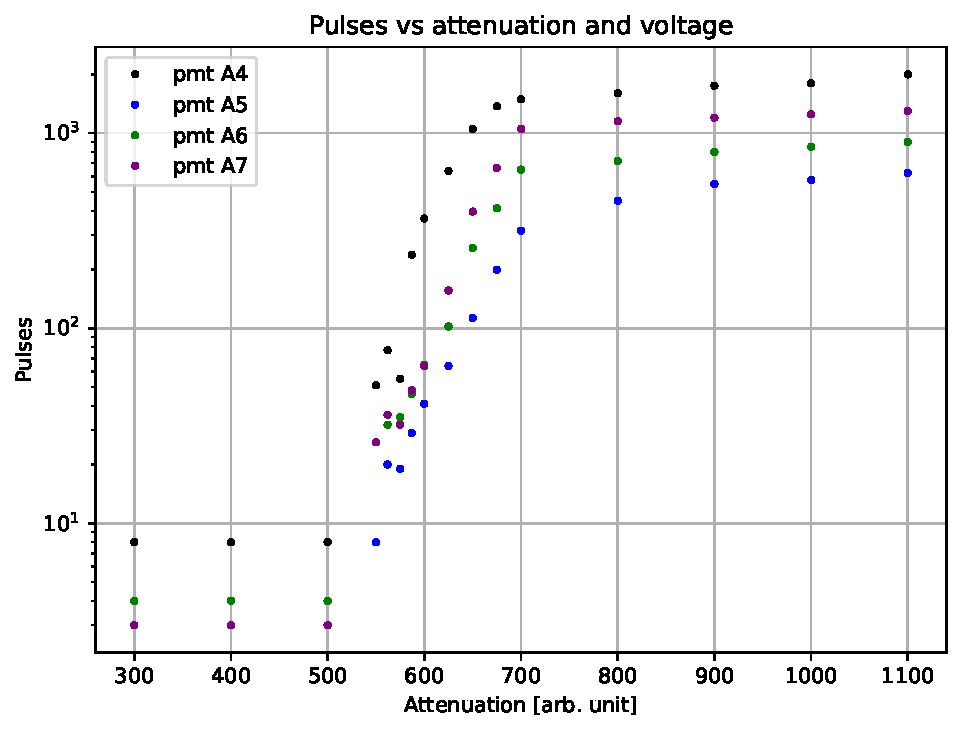
\includegraphics[width = 0.5\textwidth]{Analysis/AttenuationA(4-7).pdf}
\caption{Attenuation scan for Detector A, for the pmt 4-5-6-7}
\end{figure}

We repeat the same test of detector B also for this 4 pmts, without finding any problem or strange behavior. The same procedure was repeated also for the last 3 Pmts of detector A, we took as above 10 acquisitions 1 minute long to study the count distribution, with one pmt in coincidence:

\begin{center}
\begin{tabular}{|c|c|c|c|c|}
\hline 
pmt & 2 & 1 & 0 & (in coincidence) \\ 
\hline 
1 & 91 & 51 & 50 & 27 \\ 
\hline 
2 & 86 & 61 & 50 & 7 \\ 
\hline 
3 & 58 & 48 & 45 & 18 \\ 
\hline 
4 & 95 & 62 & 41 & 29 \\ 
\hline 
5 & 69 & 60 & 50 & 21 \\ 
\hline 
6 & 85 & 57 & 45 & 19 \\ 
\hline 
7 & 66 & 51 & 46 & 28 \\ 
\hline 
8 & 74 & 51 & 48 & 22 \\ 
\hline 
9 & 77 & 43 & 45 & 17 \\ 
\hline 
10 & 62 & 44 & 50 & 29 \\ 
\hline 
\end{tabular} 
\end{center}

\begin{equation*}
\begin{split}
\mu_{2} = 76.3 \qquad \sigma^{2} = 160  \\
\mu_{1} = 52.8 \qquad \sigma^{2} = 47.5 \\
\mu_{0} = 47.0 \qquad \sigma^{2} = 9.6  \\
\mu_{4} = 21.7 \qquad \sigma^{2} = 48.2 \\
\end{split}
\end{equation*}

For these 4 pmts, $\sigma^{2}$ is different from the expected mean, this doesn't agree with the hypothesis that the count are Poisson distributed, we can quantify this with a statistical test: in this table the correlation matrix:

\begingroup
\setlength{\tabcolsep}{8pt} % Default value: 6pt
\renewcommand{\arraystretch}{1.2} % Default value: 1
\begin{center}
\begin{tabular}{|c|c|c|c|c|}
\hline 
Pmt: & 2 & 1 & 0 & pmt in coincidence \\ 
\hline
$\chi^{2}_{9}$ & 19.6 & 8.30 & 1.90 & 39.5\\ 
\hline
\end{tabular} 
\end{center}
\endgroup
\smallskip

The expected error for the result of this test is $\sigma = \sqrt{2*(n-1)} \simeq 4$. In this case we are observing 3 values that are more than  $3 \cdot \sigma$ far from the expected value. If we look at the correlation matrix :

\begin{center}
\begin{tabular}{|c|c|c|c|c|}
\hline 
pmt: & c & 0 & 1 & 2 \\ 
\hline 
c 	 & 1 & -0.18  & -0.21  & -0.06  \\ 
\hline 
0 	 & -0.18  & 1 & -0.10  & -0.22  \\ 
\hline 
1    & -0.21  & -0.10  & 1 & 0.56  \\ 
\hline 
2    & -0.06 & -0.22  & 0.56  & 1 \\ 
\hline 
\end{tabular} 
\end{center}


We observe negative correlation between the pmts, something not expected. After some investigations, we find out that the program which controls the NINO board had a bug: the program partially overwrote some detector B settings for detector A as well. Since detector B has only three pmt's, the problem affected the PMT's with the same numbering as detector A. After fixing this issue we repeated the same test, without finding any problem. 

\section{Calibrations.}

One of the main goal for this experiment was to measure the well know trasverse asymmetry of $^{12}C$, already measured before, as a test for the new electronic system. Previous measurements of the Transverse asymmetry have been performed for a carbon target. For this beam-time, the two spektrometers were placed at an angle such that the $Q^{2}$ values of the scattered electron is:

\begin{flushleft}
\begin{align*}
& det. A : \qquad Q^{2} = \SI{0.041337}{\giga \electronvolt \squared} \qquad \textnormal{without Cut} \\
& det. A : \qquad Q^{2} = \SI{0.0394513}{\giga \electronvolt \squared} \qquad \textnormal{with Cut} \\
& det. B : \qquad Q^{2} = \SI{0.0404771}{\giga \electronvolt \squared} \qquad \textnormal{without Cut} \\
& det. B : \qquad Q^{2} = \SI{0.0405843}{\giga \electronvolt \squared} \qquad \textnormal{with Cut} 
\end{align*} 
\end{flushleft}

The $Q^{2}$ values is the same of the last measurement performed at MAMI, and is measured with and without rejecting the inelastic electrons. 

\subsection{Alignment of the scattering plane.}

\subsection{Beam monitors calibration, XY monitors}

For the calibration of the X Y monitors, special target are used. In the target frame (\ref{fig:targetFrame}) there are two targets made by three carbon wires that are at a fixed distance each other, horizontally and vertically aligned. The distance between the center of the two external wires is measured, and it is equal to $ d_{horizontal} = \SI{2.38}{\milli \meter}$ for the horizontal wires and $d_{vertical} = \SI{2.33}{\milli \meter}$ for the other one.
The procedure to retrieve the correct scaling factor, to convert from the raw-data in $\SI{}{\volt}$ to $\SI{}{\micro \meter}$, is the following: we ask MAMI operators to slowly change the beam position, in the horizontal and vertical direction for the horizontal and vertical target. The beam position can be changed by varying the Magnetic field produced by the \textit{Wobbler 16} magnets (\ref{fig:BeamLine}). 
During this slow variation, our detectors are measuring the rates of scattered electrons, that increase when the beam hit one of the three wires and and decrease when the beam is centered between two wires. We plot the detector counts versus the $XY$ monitors values, in voltage, and we estimate the position given in voltage of the two external peaks. This values can be used, together with the distance $d_{horizontal};d_{vertical}$ already measured, to compute the scaling factors. This procedure is repeated for $X21/Y21$ and $X25/Y25$ monitors.


\begin{figure}[htb]
%\setlength{\columnsep}{10pt}%
\centering
\includegraphics[width = 0.40\textwidth]{ExperimentalSetup/target.pdf}
\caption{Target frame installed during the experiment, on the top we have the two targets made by three carbon wires that are used to calibrate the positions monitors. Then the carbon target and the two lead targets.}
\label{fig:targetFrame}
\end{figure}

Looking at the PMT counts, we observe that the counts increase to a maximum, that is reached when the beam spot is centered on the carbon wire, and then decrease until the next carbon wire is hit by the beam.\\
We plot the pmt data \textit{versus} the $X25,X21,Y25,Y21$, given in $\SI{}{\volt}$. 
Given that we know the real distance between the two external wires, we can obtain the correct scaling factors to calculate the X and Y position from the voltage values. To identify the three peaks in of the carbon target, we fit the data using a gaussian model (see \ref{fig:HorizontalCalibration}). The mean $\mu$ represents the center of the wire, given in $\SI{}{\volt}$.


\begin{figure}[hbtp]
\centering
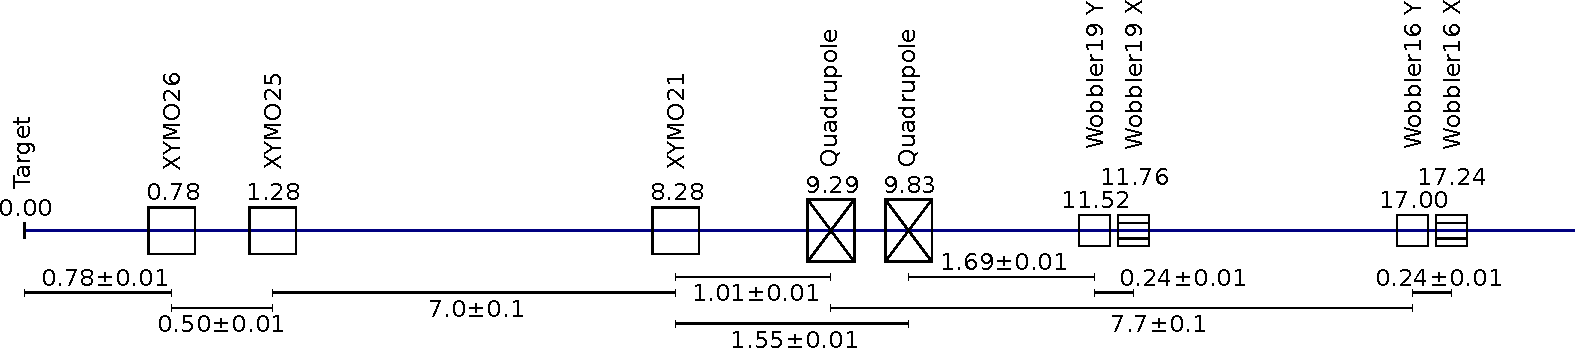
\includegraphics[scale=0.4]{figures/XYMOCalibBeamLine.pdf}
\caption{Beam line scheme.}
\label{fig:BeamLine}
\end{figure}


Looking at the Beam line, we assume that the beam travels in a straight line. Let's consider the \textit{Wobbler 16} magnet the "$0$" of a coordinate system, with the $z$ axis pointing to the target (left direction in the beam scheme). The Beam parameters are measured by the Monitors $X/Y_{21}, X/Y_{25}$, which are located at some distance respect to the target. Suppose we are working only with the $Y_{25}$ monitor (the procedure is the same for the others). The Beam $y$ position is described by:

\begin{align*}
y_{beam} = m \cdot (z - z_{wobbler 16})
\end{align*}

In the scheme \ref{fig:BeamLine} we easily compute the distance between the $Y_{25}$ monitor and the \textit{wobbler 16} magnet, so we have the slope $m$. The Position on the target is given by $Y_{target} = m \cdot Z_{target}$. With these simple equations then:

\begin{equation}
c_{Y25} = \dfrac{d_{vertical} [\SI{}{\milli \meter}]}{ Y_{target}} 
\end{equation}

$c_{Y25}$ indicates the scaling factor of the monitor. With these values the Analysis program compute the correct beam position, and from that the incident angles in the $x,y$ directions, which are needed later for the analysis.

\begin{figure}[hbtp]
\centering
\subfloat[][]{
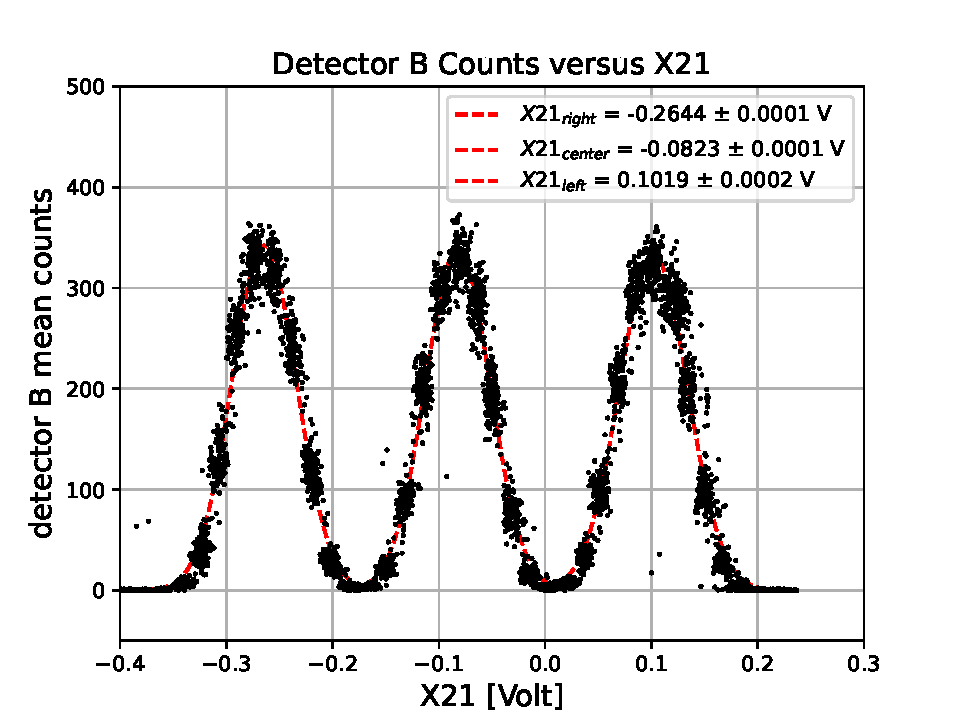
\includegraphics[width=0.4\textwidth]{Analysis/HorizontalCalibration.pdf}}
\subfloat[][]{
\includegraphics[width=0.4\textwidth]{Analysis/HorizontalCalibrationX25.pdf}}
\caption{Plot of the averaged count of detector B, with the slow variations of the beam position in the horizontal direction. The three peaks occur when the beam is aligned with the center of the wire. The values on the X axis are in $\SI{}{\volt}$}
\label{fig:HorizontalCalibration}
\end{figure}

All this procedure can be  checked if we plot now the $X$ and $Y$ position for the same two runs of data acquired with the wires. After placing the scaling factors obtained in the standard configuration file, we run the analysis another time and the physical values were computed \ref{fig:CheckHori}

\begin{figure}[hbtp]
\centering
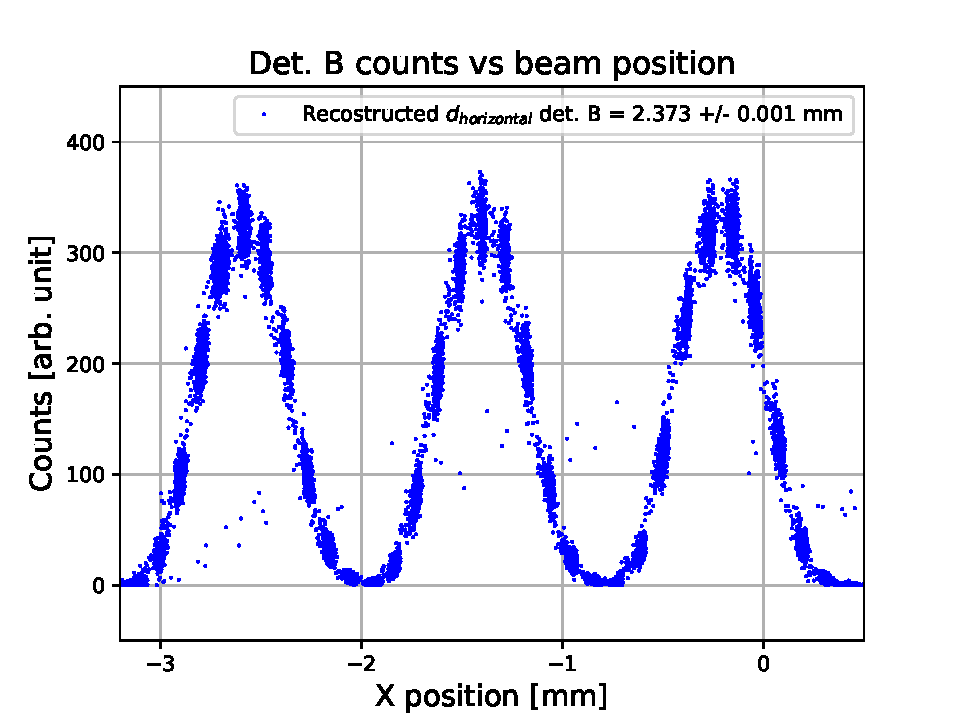
\includegraphics[width=0.45\textwidth]{Analysis/XcheckB.pdf} 
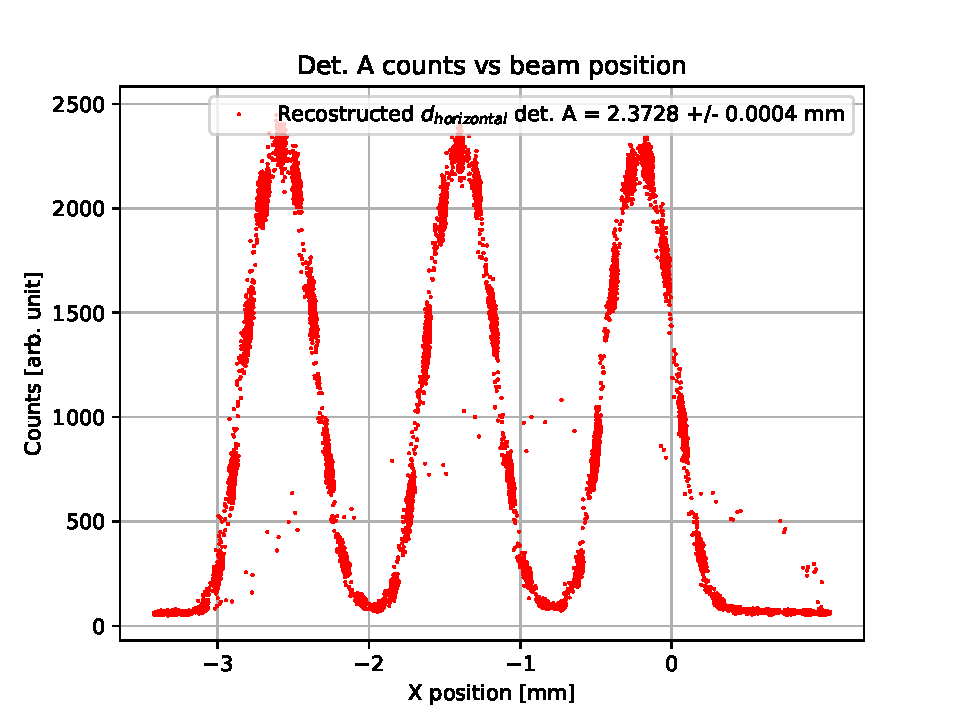
\includegraphics[width=0.45\textwidth]{Analysis/XcheckA.pdf}
\caption{plot of the PMT Count against the physical values computed by the analysis program. Now the position of the three peaks correspond to the expected values measured for the target.}
\label{fig:CheckHori}
\end{figure}
\newpage

\subsection{Current (PIMO) and energy monitors (ENMO) calibration.} \label{CurrentCalibration}

The last two calibration needed for the analysis are about the energy and the current intensity of the beam, which are indicated with PIMO (current monitor) and ENMO (energy monitor). 
The values that we measure are given by VFCs counts. We remind the reader how the VFCs monitors operate: the input signal from the beam is transformed in a pulse wave whose frequency is proportional to the input voltage.  The signal is so proportional to various quantities that we want to measure, however we need to determine the correct scaling factor and possible offsets to conver these quantities in physical units ready for the analysis. For this beam time the current is measured in $\SI{}{\micro \ampere}$ and the beam energy is given in $\SI{}{\electronvolt}$.\smallskip

For the current monitors I13 and I21, the raw counts are converted in digitalized voltage values with the formula shown in (\ref{eq:Vfc}). The relation between these values given in $\SI{}{\volt}$ and the real values in $\SI{}{\micro \ampere}$ and $\SI{}{\electronvolt}$ is linear:
\begin{align*}
I(\SI{}{\micro \ampere}) = m I(\SI{}{\volt}) + q
\end{align*}

To determine the two coefficients, the beam current was raised from $\SI{10}{\micro \ampere}$ to $\SI{22}{\micro \ampere}$ in several step. For each step we confront the nominal values of the current with the values in $\SI{}{\volt}$ measured. The following plot show the procedure described:

\begin{figure}[ht]
\centering
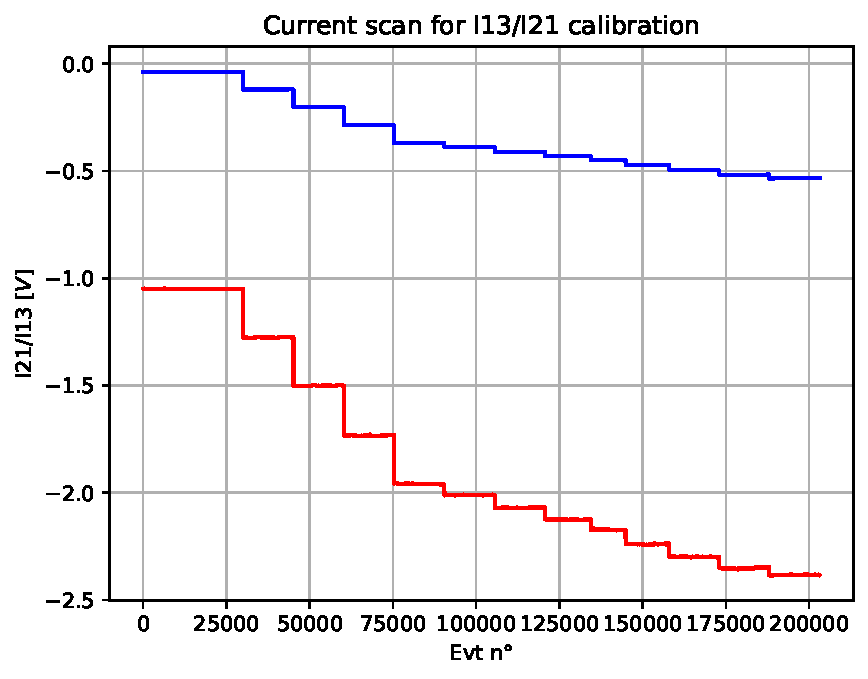
\includegraphics[width = 0.5\textwidth]{Analysis/Calibrations/ScanI21I13.pdf}
\caption{Current scan for the calibration, each step correspond to a run with a different beam current.}
\label{fig:ScanCurrent}
\end{figure}

The calibrations consist in retrieving $m$ and $q$ with a linear fit. Then the parameters are added in the standard configuration file, together with the other calibration parameters, and can be loaded by the analysis program to process the data.  

\begin{figure}[hbtp]
\centering
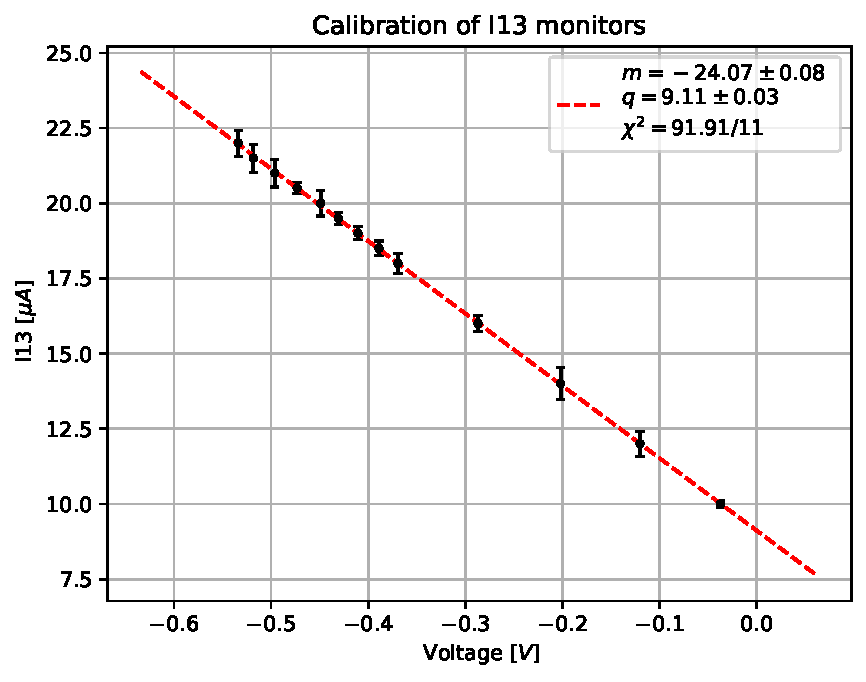
\includegraphics[width = 0.45\textwidth]{Analysis/Calibrations/I13.pdf}
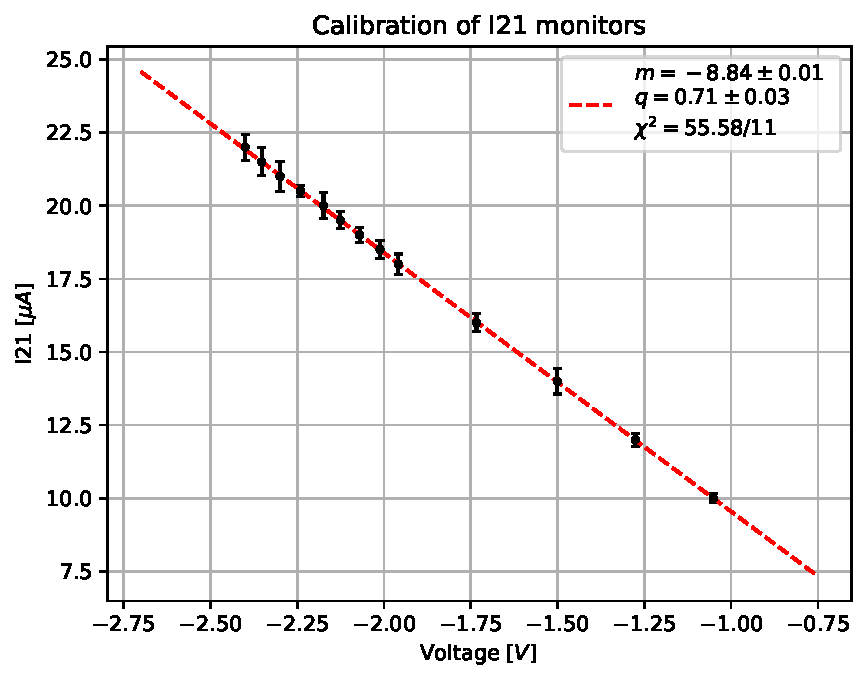
\includegraphics[width = 0.45\textwidth]{Analysis/Calibrations/I21.pdf} 
\caption{Calibrations plots for PIMO I21 and PIMO I13, the errors are multiplied by $25$.}
\label{fig:PimoCalib}
\end{figure}

The values obtained from the fit of nominal beam current vs. voltage values are shown in the figure \ref{fig:PimoCalib}. The $\chi^{2}$ values are higher than the expected. This is not unexpected, the errors in both the plots are computed with the sampling standard deviation formula applied to the sequence of voltage values $I21\/ I13$ ($\sigma_{vfc}$, the standard deviation computed for each step in \ref{fig:ScanCurrent}), and it is related to precision of the analog to digital converter VFCs. The errors are then propagated to the $y$ axis showed in the plot. \smallskip
Yet, we are underestimating the error associated with nominal current $I$, in fact the accuracy associated with the beam current, set by the accelerator operators, was not disclosed, and we suspect that is not negligible compared to $\sigma_{vfc}$. \bigskip  

The ENMO calibration is performed in a different way from the other monitors. The energy calibrations is made with a particular procedure that is automatically made by MAMI operators, and exploit the polarity signal which controls the beam polarization at the source of the acceleration. Mami operators use the signal to create artificially a difference in the beam energy that is correlated to the beam polarity. This difference is equal (nominal) to $\SI{22.6}{\kilo \electronvolt}$, and consist in the last two sub-events with higher energy respect to the first two. Because we know the nominal difference, the calibration consist in computing the correct scaling factor which convert from $\SI{}{\volt}$ to $\SI{}{\kilo \electronvolt}$. The quantity that is relevant for the calibration is $\delta E$ (with $E_{18}$ being the energy monitor):

\begin{equation*}
\delta E = \frac{E_{18}[3] + E_{18}[3]}{2} - \frac{E_{18}[0] + E_{18}[1]}{2} 
\end{equation*}

An histogram of $\delta E$ should show a single peak whose values correspond to $\SI{22.6}{\kilo \electronvolt}$.
For this calibration, we took 3 different acquisition, which differ for the different values of the beam current. We remind that the output voltage signal from the XY monitor is proportional to the current, as mentioned in \ref{eq:SignalToVfc}, so we have that:

\begin{equation}
U[\SI{}{\volt}] = \frac{1}{C_{E18}} \, \cdot  i \cdot E
\end{equation}

So, if we invert the relation we have that:

\begin{equation}
\frac{E}{U} = C_{E18} \, \cdot \frac{1}{i} \qquad  C_{18} = \frac{E}{U} \, \cdot i
\end{equation}  

And we have the scaling factor.

\begin{figure}[hbtp]
\centering
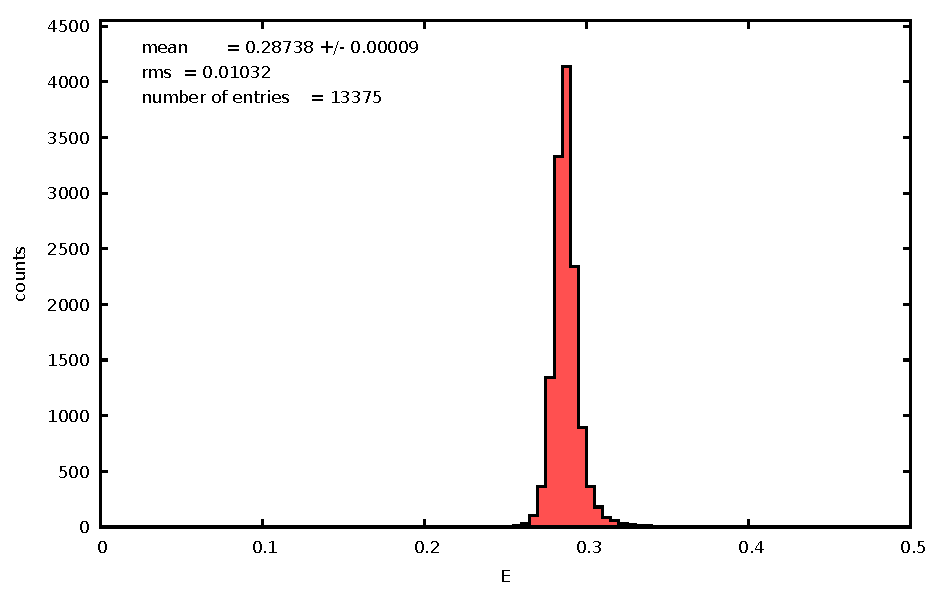
\includegraphics[width = 0.45\textwidth]{Analysis/ENMOvoltage20.pdf}
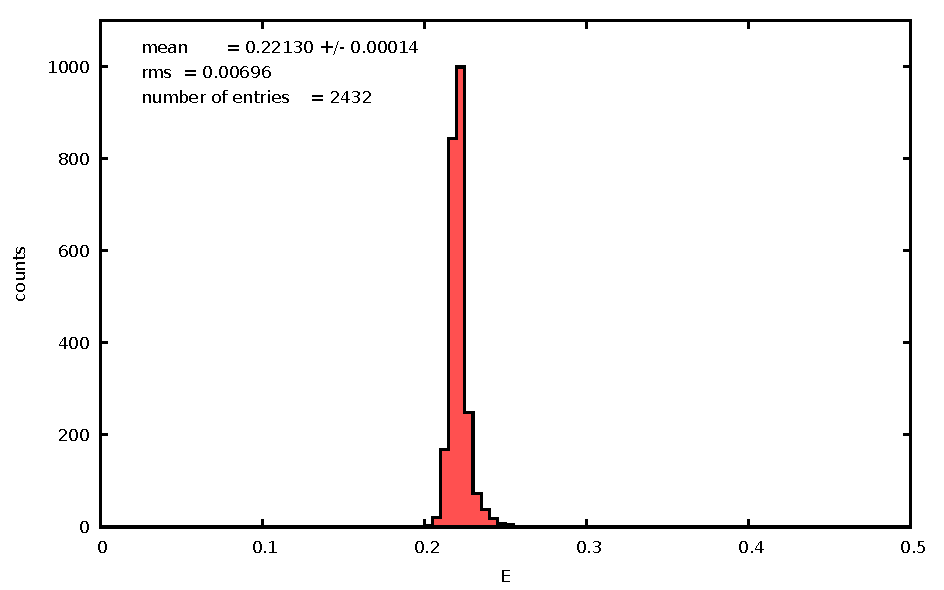
\includegraphics[width = 0.45\textwidth]{Analysis/ENMOvoltage15.pdf} 
\caption{Histograms or $\delta E$ with the beam current $\SI{20}{\micro \ampere}$ on the left and $\SI{15}{\micro \ampere}$ on the right.}
\end{figure}


\begin{figure}[hbtp]
\centering
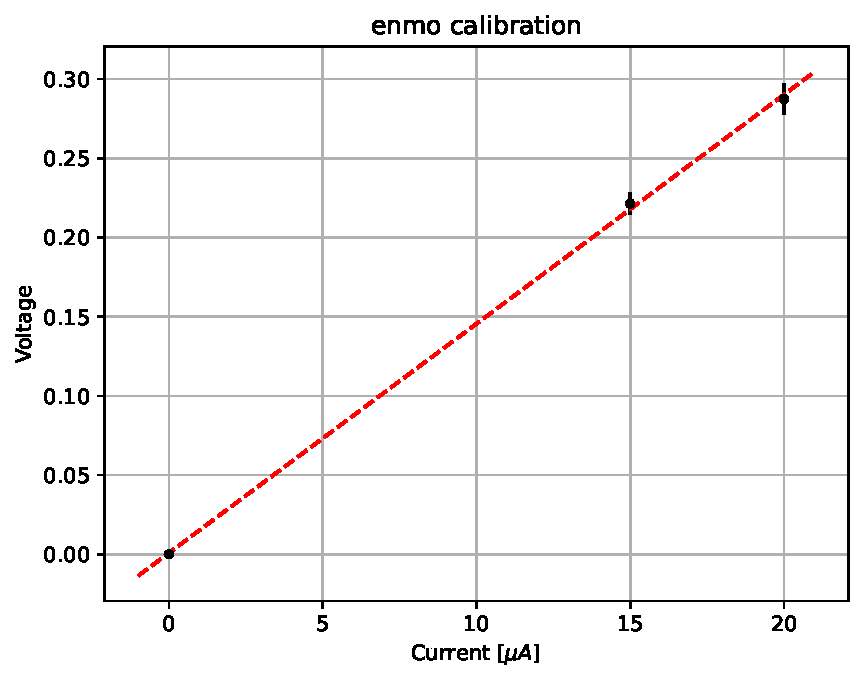
\includegraphics[width = 0.5\textwidth]{Analysis/Calibrations/E18_Calibration.pdf}
\caption{Calibration of ENMO monitor, plot of the ENMO voltage values versus the current.}
\end{figure}


$C_{E18}$ is obtained taking the coefficient parameter $m$ from the fit and substituting in:

\begin{align*}
C_{E18} =  \frac{\SI{22.6}{\kilo \electronvolt}}{m}
\end{align*}

From this we obtain the value $C_{E18} = +1595.2$ necessary to convert from Voltage units to $\SI{}{\kilo \electronvolt}$. Using the value, we can show an histogram of $\delta E$ in physical units, as a check of our procedure:

\begin{figure}[hbtp]
\centering
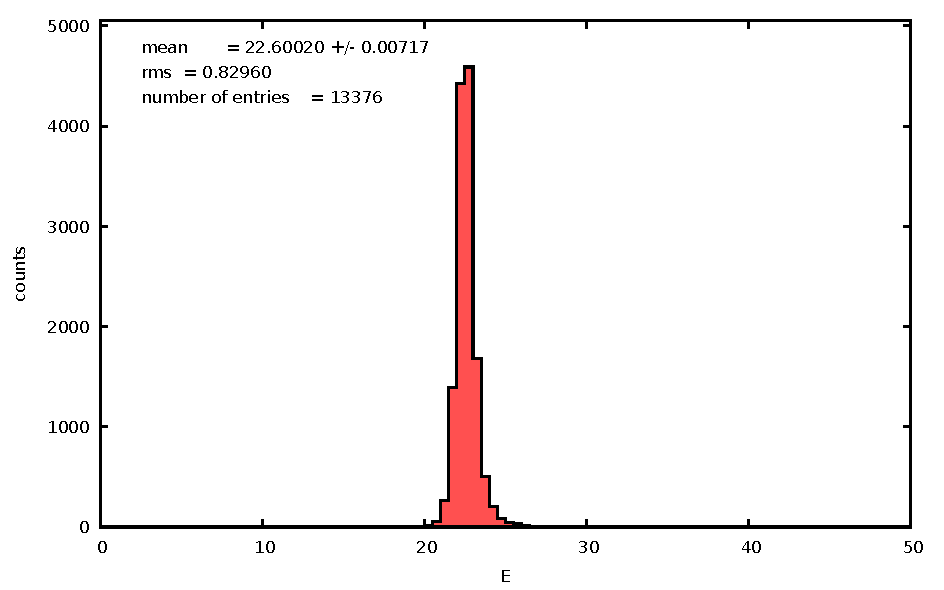
\includegraphics[width = 0.45\textwidth]{Analysis/ENMOCheck20.pdf}
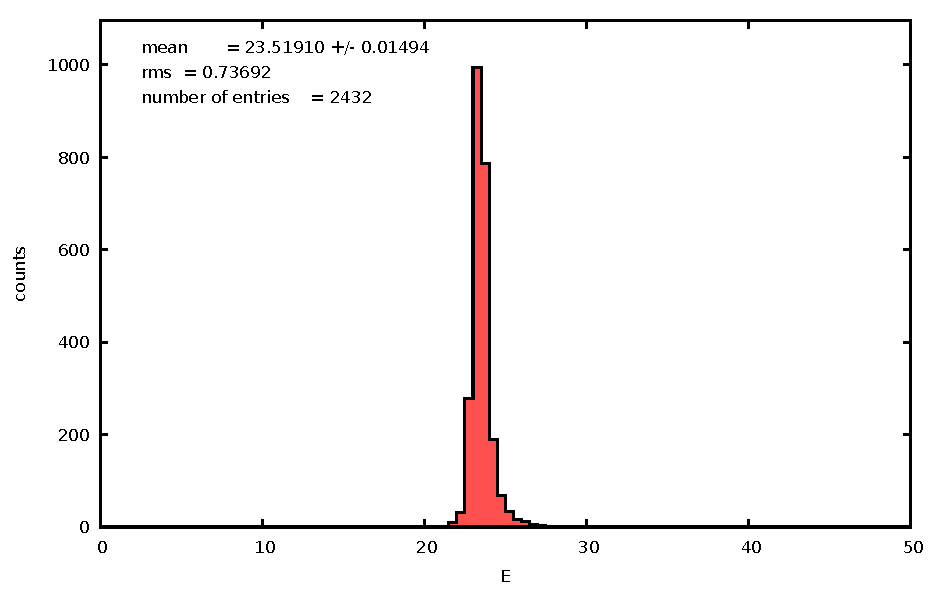
\includegraphics[width = 0.45\textwidth]{Analysis/ENMOCheck15.pdf} 
\caption{Plot for the physical quantities computed in the data tree, for two different current of the beam (on the left $\SI{20}{\micro \ampere}$, $\SI{15}{\micro \ampere}$ on the right)}
\end{figure}

\subsection{Calibration of the PMTs}

\commento{Here it's important to show the plots I made during the beam time. I have to mention the Leo tecniques for the correct interpretation of counts vs attenuation.}

During the beam time, several scans in attenuation were performed, before switching MAMI to produce the polarized beam, to choose the best working point for the PMTS of the detectors. The same procedure used in the laboratory was followed, so with a beam intensity of $\SI{10}{\micro \ampere}$ we acquire data run one minute long, increasing each time the attenuation.

\begin{figure}[hbtp]
\centering
\subfloat[][\emph{Attenuation scan for the PMTs of detector B} \label{fig:AttScan}]
{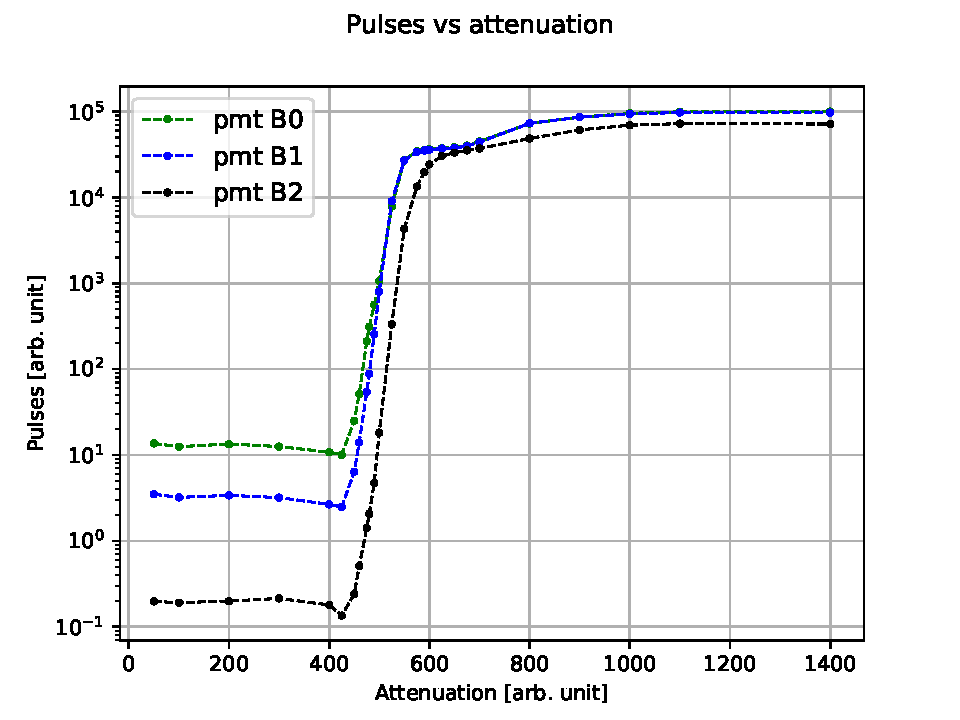
\includegraphics[width = 0.5\textwidth]{Analysis/CalibrationPMT/AttenuationScanB.pdf}}
\subfloat[][\emph{Attenuation scan for the PMTs of detector B}]
{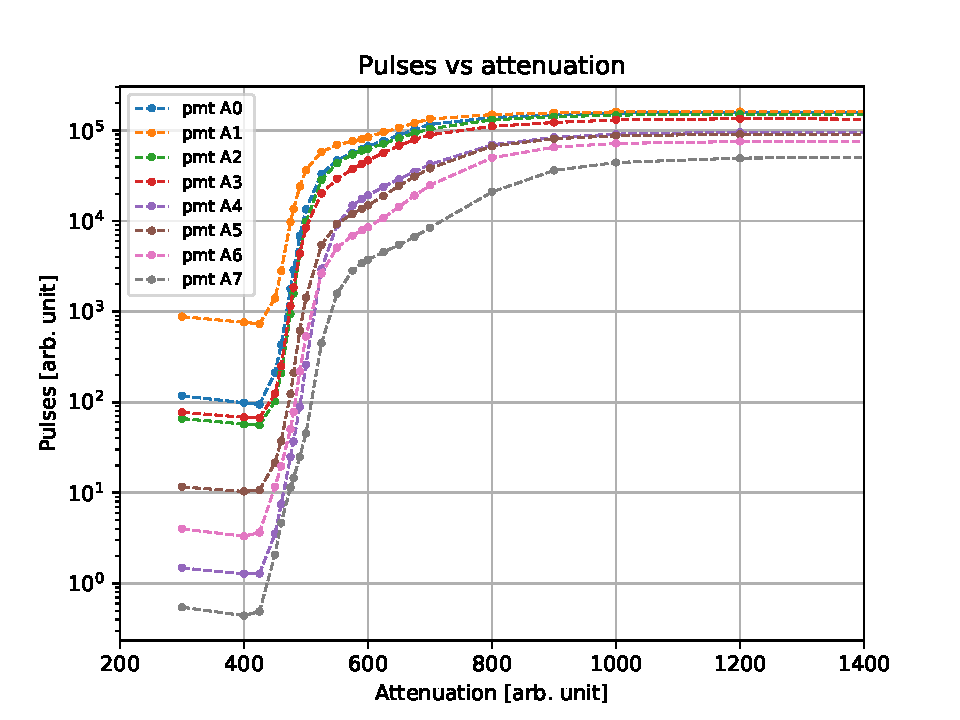
\includegraphics[width = 0.5\textwidth]{Analysis/CalibrationPMT/AttenuationScanA.pdf}}
\end{figure}


From the fit we obtain three valus for the signal Peak, given in attenuaton units.
We can check the idea behind this, visualizing the PMT count in a different way. Because we would like to visualize the number of electrons that generate a certain signal in the detector, we can think of differentiating the data showed in the plot \ref{fig:AttScan}. The differentiation consist in the difference between the Counts at a certain point and the previous one, and dividing by the increment in attenuation:

\begin{align*}
Spectra = \frac{N(att_{i}) - N(att_{i-1})}{att_{i} - att_{i-1}} 
\end{align*}

\begin{figure}
\centering
\subfloat[][\emph{B0} \label{fig:Spectra}]
{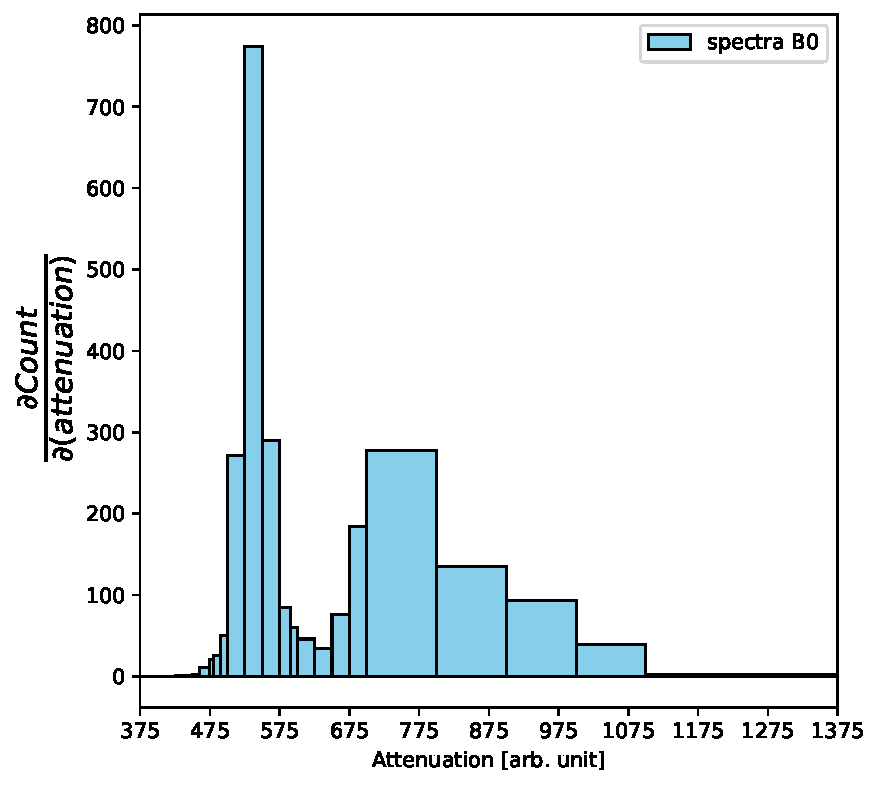
\includegraphics[scale = 0.5]{Analysis/CalibrationPMT/B0.pdf}}
\subfloat[][\emph{B1}]
{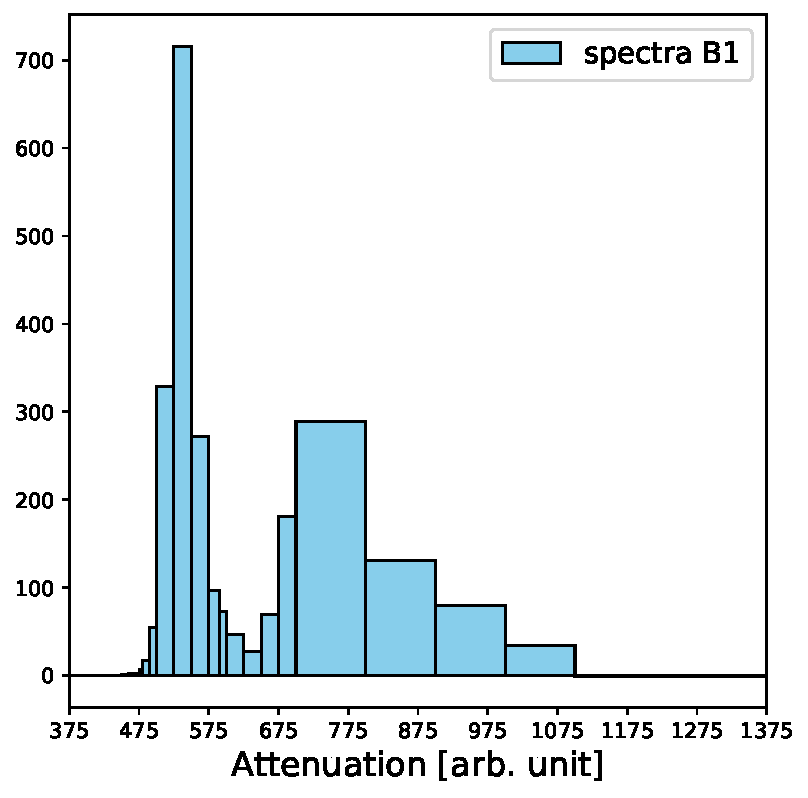
\includegraphics[scale = 0.5]{Analysis/CalibrationPMT/B1.pdf}}\\
\subfloat[][\emph{B2}]
{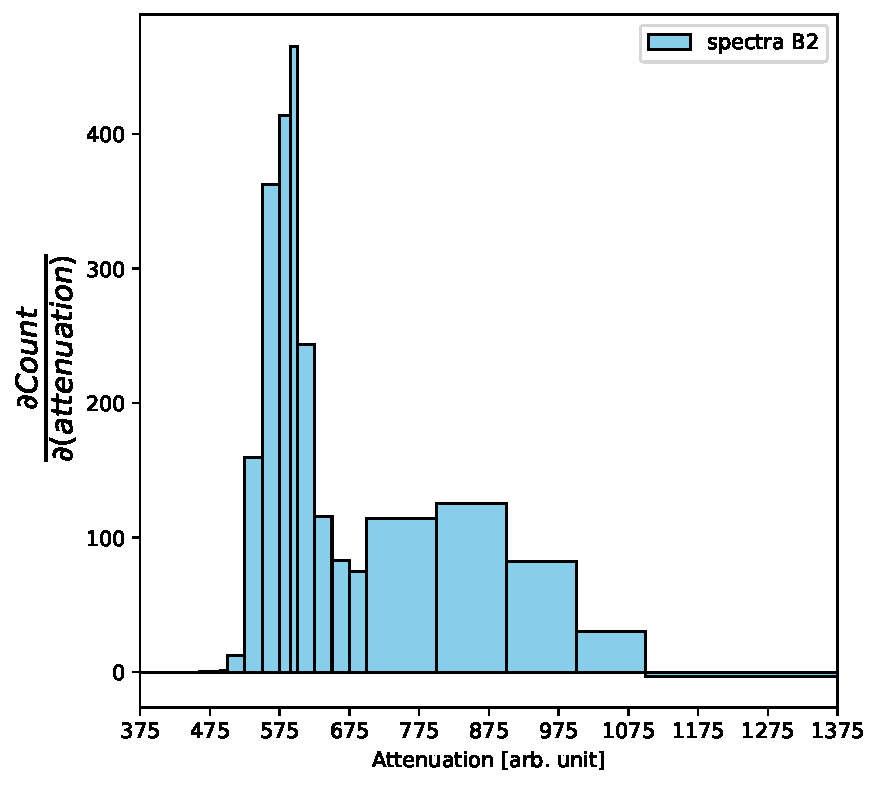
\includegraphics[scale = 0.5]{Analysis/CalibrationPMT/B2.pdf}}
\caption{Reconstructed spectra for Detector B}
\end{figure}

In this way we compute a discrete derivative of the plot showed in \ref{fig:AttScan}, which represent $\frac{\partial N}{\partial att}$. This is, in fact, the spectra of the signal, still given in attenuation units \ref{fig:Spectra}.
This plot are used to identify a good point to select the attenuation values. If we look at the plots \ref{fig:ThrvsAtt}, we can see that the physical threshold does not scale linearly with changing the attenuation value, and for high values of attenuation, the threshold falls quickly at zero. 
Looking at the signal spectra, we identify the first peak as the electron signal. The other peak, for higher attenuation values (on the right), correspond to very low threshold values, and it is identified as the background noise. 
We selected the values of the attenuation between the peaks of the two distributions, maximizing the signal acceptance and trying to reject the background as much as possible.
Our discussion so far is sufficient to carry out the calibration of the PMTs and take data to measure the asymmetry. However, we would like to identify the physical threshold in $\SI{}{\milli \volt}$ instead of attenuation unit. We can use the conversion function that we discussed in \ref{fig:ThrvsAtt}:

\begin{align*}
f(att) = \dfrac{a}{(x - b)^{3} + d}
\end{align*} 

We point out that the parameters of this function have been obtained from data that have not been acquired during this thesis work, moreover the threshold value in the program that controls the NINO board is slightly different (we always used 600, the data are taken with 750), therefore the values in volts need probably to be rescaled by some factor, but for our discussion we are interested in a raw estimation of the signal peak:
With this conversion, we show the same plots in \ref{fig:Spectra}, with the values in the x-axis in $\SI{}{\volt}$ now.

\begin{figure}[h]
\centering
\subfloat[][]{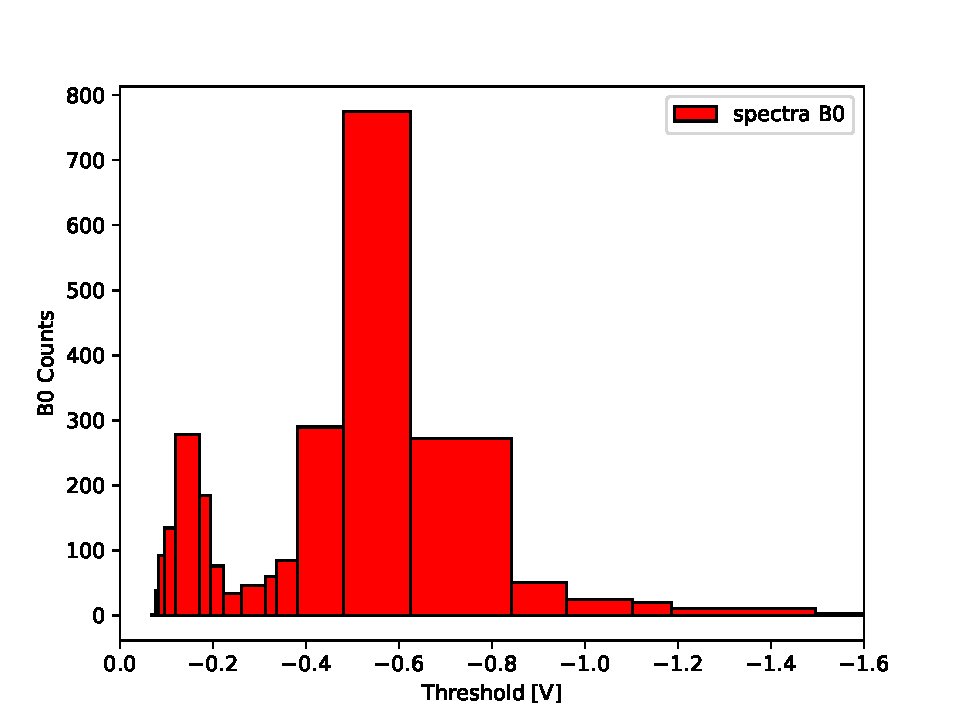
\includegraphics[width = 0.45\textwidth]{Analysis/CalibrationPMT/voltB0.pdf} }
\subfloat[][]{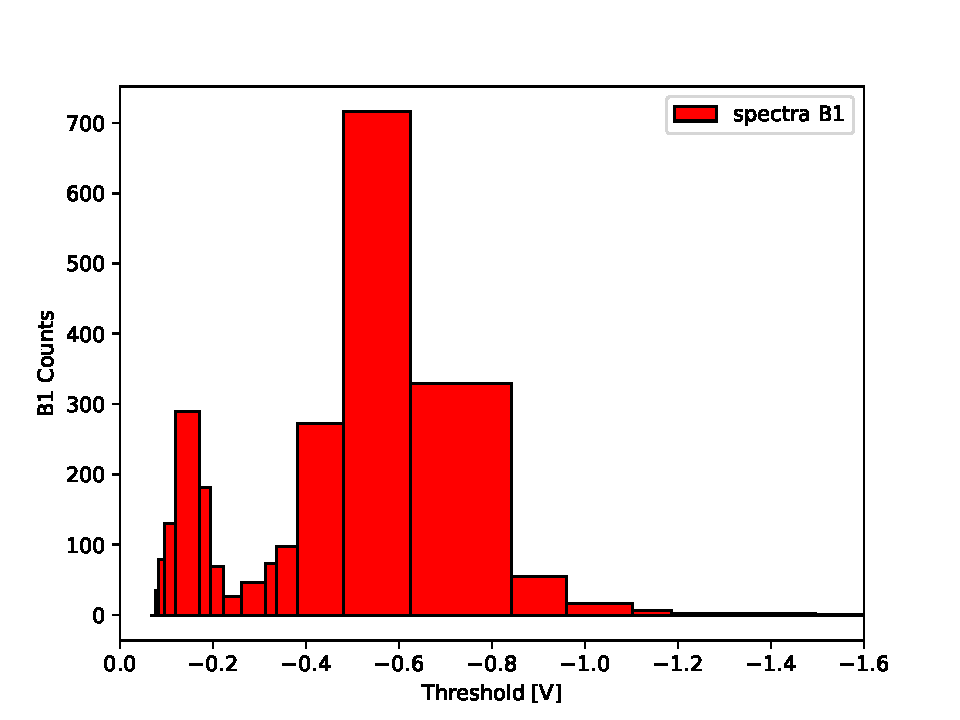
\includegraphics[width = 0.45\textwidth]{Analysis/CalibrationPMT/voltB1.pdf} }\\
\subfloat[][]{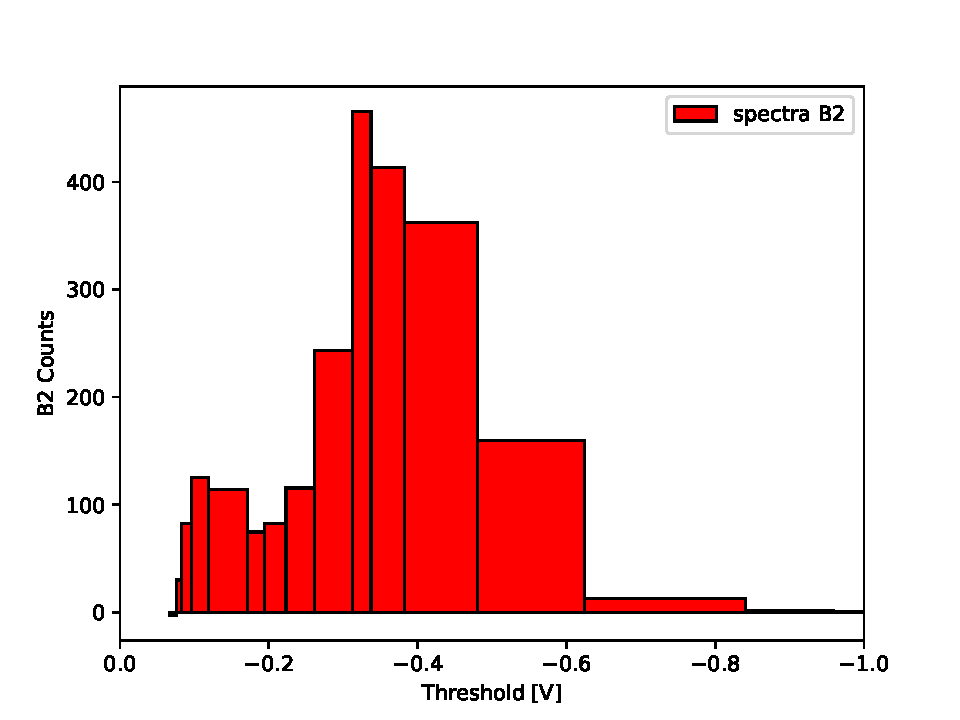
\includegraphics[width = 0.45\textwidth ]{Analysis/CalibrationPMT/voltB2.pdf} }
\end{figure}

We know see clearly two peaks, the signal and the background, that are reversed respect to \ref{fig:Spectra}.

We discuss now a simple model that we used to describe how the PMT Counts vary when we raise the attenuation. From \ref{fig:Spectra}, we assume that the two peaks are described by two gaussian distributions. Now if we think about the the probability for a signal to pass the selection, this quantity is equal to the probability of being in below the attenuation value. Using now the fact that the probability are given by the cumulative of the gaussian distribution (probability of being in the right tail) it is straightforward to deduce:

\begin{align*}
P(signal > thr) = \, \Phi(x) = \dfrac{1 + Erf(\dfrac{x - \mu}{\sqrt{2} \sigma })}{2}
\end{align*}

Considering that we have the sum of two gaussian distribution, we end with:

\begin{equation}
\begin{split}
N(att) = \frac{n_{1} + n_{2}}{2} + (\frac{n_{1}}{2}) Erf(\dfrac{x - \mu_{1}}{\sqrt{2} \sigma_{1} })   + (\frac{n_{2}}{2}) Erf(\dfrac{x - \mu_{2}}{\sqrt{2} \sigma_{2}}) \\
\end{split}
\end{equation}

This model is used to fit the data. The result is shown in the following picture, the parameters obtained from the fit are reported below:

\begin{figure}
\centering
\includegraphics[width = 0.65\textwidth ]{Analysis/CalibrationPMT/Fit_attenuation.pdf}
\end{figure}

\begin{table}
\centering
\begin{tabular}{c|c|c|c|c|c|c}
\hline
 PMT   &  $\mu_{1}$         &  $\sigma_{1}$         & $\mu_{2}$          & $\sigma_{2}$   & n1                & n2                 \\
\hline
 B0    & 538.0 +/- 1.3 & 19.4 +/- 1.1 & 798 +/- 8 & 103 +/- 4 & 34277 +/- 662 & 64244 +/- 1538 \\
 B1    & 536.4 +/- 0.9 & 18.2 +/- 0.7 & 783 +/- 5 & 89 +/- 2  & 34053 +/- 475 & 61636 +/- 1109 \\
 B2    & 582.8 +/- 1.2 & 25.9 +/- 1.0 & 824 +/- 8 & 88 +/- 6  & 32880 +/- 758 & 37930 +/- 1245 \\
\hline
\end{tabular}
\end{table}

From these result we measure the mean $\mu_{1}$ and $\mu_{2}$ for the signal and the background given in attenuation units. The correct value of attenuation is set between the two observed peaks, in order to rejects the background and take only the signal coming from the scattered electrons. The same procedure was followed also for the detector A, the plots are not reported here, for brevity, but in the appendix.

\subsection{Autocalibration procedure} \label{Autocalib}

In this section we present the last calibration tecniques needed in the data-process. The autocalibration is a special operation mode of the MAMI accelerator, during which the beam current is made to vary in a controlled way. Through these special runs is possible to obtain again the current scaling factor that we discussed in \ref{CurrentCalibration}. Because the current in varying, it is possible to study the linearity of the PMTs. From a linear fit of the PMTs counts vs. current intensity the angular coefficient and the offset are measured. The offset is particual important because give rise of a possible systematic error that influence the final asymmetry result. It is quite simple to demostrate this, if a relation of the type $N = mI + N_{0} $ holds. Consider the following quantity:

\begin{align*}
\overline{N} = \frac{N_{\uparrow} + N_{\downarrow}}{2}
\end{align*} 

we can express $N_{\uparrow}$ and $N_{\downarrow}$ in this way:

\begin{align*}
N_{\uparrow} = \overline{N} + A_{n}\overline{N} \\
N_{\downarrow} = \overline{N} - A_{n}\overline{N} 
\end{align*}

Now we suppose that $\overline{N}$ is linear dependent on the current in the way we defined above, so:

\begin{align*}
N_{\uparrow} = \overline{N} + A_{n}(mI) + N_{0} \\
N_{\downarrow} = \overline{N} - A_{n}(mI) + N_{0} 
\end{align*}

We are supposing that the offset $N_{0}$, we assume that the present offset does not contribute to the asymmetry, i.e. it is not correlated to the signal of the scattered electrons, but is due to processes of another type, therefore in the previous formulas only the $mI$ counts must be multiplied by the asymmetry $A_{n}$. Therefore if we substitute everything in the definition of the transverse asymmetry:

\begin{equation} \label{eq:Systematic}
A^{'} = \dfrac{N_{\uparrow} - N{\downarrow}}{N_{\uparrow} + N{\downarrow}} = \dfrac{A_{n} (2mI)}{ (2mI) + 2N_{0} } = A_{n} \dfrac{1}{1 + \frac{N_{0}}{mI}}
\end{equation} 

In the last passage we learn that the presence of an offset can decrease the recostructed asymmetry. So it's important to determine quantitatively $N_{0}$ and $m$ in order to be able to take care of this effect. The strategy used is quite simple: every three hours of production data, we asked MAMI to start the autocalibration program. With all the autocalibration runs, we estimate $N_{0}$ for each PMT, separately. Then All this quantities are saved in a file so that the analysis program can retrieve the parameters and subtract them from the PMT counts. \medskip
In this way every three hours the PMT are corrected, this take care also of the possibility that the the linearity of the PMTs can change after hours of use of the PMTs (for example it can decrease the efficiency).

During the autocalibration, the beam current is raised from $\SI{9}{\micro \ampere}$ to $\SI{11.125}{\micro \ampere}$ in step of $\SI{0.125}{\micro \ampere}$:

\begin{figure}[ht]
\centering
\subfloat[][\emph{Autocalibration: in this plot we have the voltage value of I21 monitor. The current is first stabilized around $\SI{10}{\micro \ampere}$, then it is raised from $\SI{9}{\micro \ampere}$ (the step lower down) to $\SI{11.125}{\micro \ampere}$ in step of $\SI{0.125}{\micro \ampere}$.} \label{fig:Autocalibration}]{
\includegraphics[width = 0.75\textwidth]{Analysis/Autocalib/Current.pdf}}
\end{figure}

With a linear fit we can estimate the scale and the offset to convert from I21 voltage values to physical values of the current. The procedure in repeated for the $8$ autocalibration acquisition we had during the beam time, so we can also take care of possible variations during the time.

\begin{figure}[ht]
\centering
\subfloat[][\emph{Current scan for detector B, the error are multiplied by a factor of $20$.}]{
\includegraphics[width = 0.5\textwidth]{Analysis/Autocalib/fitB.pdf}} \\
\end{figure}

\begin{figure}[hbtp]
\centering
\subfloat[][\emph{Current scan for detector A, the error are \\ multiplied by a factor of $20$.}]{
\includegraphics[width = 0.49\textwidth]{Analysis/Autocalib/fitA0-3.pdf}}
\subfloat[][\emph{Current scan for detector A, the error are \\ multiplied by a factor of $20$.}]{
\includegraphics[width = 0.49\textwidth]{Analysis/Autocalib/fitA4-7.pdf}}
\caption{PMT Rates vs current (from I21 monitor), the model used for the fit: $y = mx + q$.}
\end{figure}

\newpage
The figures are referred to the data acquired for the first autocalibration. It's interesting to calculate, from the result of the fit, the factor that appears in \ref{eq:Systematic}:

\begin{table}[ht]
\centering
\begin{tabular}{c|c|c|c}
\hline
 PMT & m [$\SI{}{\micro \ampere}^{-1}$] & Offset & c  \\
\hline
 B0  & 1750 &  1301 &  0.93 \\
 B1  & 1742 &  1283 &  0.93 \\
 B2  & 1406 &   717 &  0.95 \\
 A0  & 6423 & 20385 &  0.75 \\
 A1  & 6756 & 29187 &  0.70 \\
 A2  & 6032 & 20513 &  0.75 \\
 A3  & 5218 & 12995 &  0.80 \\
 A4  & 3945 &  6666 &  0.86 \\
 A5  & 3967 &  6547 &  0.86 \\
 A6  & 3258 &  4655 &  0.87 \\
 A7  & 2325 &  2233 &  0.91 \\
\hline
\end{tabular}
\end{table}
Ignoring the presence of the offset lead two consequences: the recostructed asymmetry is lower, on average $ \simeq 10\%$ less than expected, and the Counts are overstimated. Because the error depend on the PMT counts, as seen in \ref{eq:Error}, this two effect combined add up and worsen the precision and accuracy of the measurement.\\
The result reported in the table can be confronted with the final result that are reported in \ref{result}. 

\newpage



\chapter{Asymmetry on Carbon and Rates on Lead target.}

\paragraph{introduction}
After having described all the calibrations needed, we are ready to analyze the data and measure the \transv from the data collected in second part of the beam time. In this chapter we explain the procedure for the pre-selection of the data (for example the removal of the events with large variation of the beam parameters) and the procedure used to analyze the recostructed asymmetry in order to obtain in the end a point exstimation for $A_{n}$. A section is dedicate to the measurement performed with lead target: the experimental rates measure using the detectors setup described here (\commento{mettere riferimento}) are reported; through the knowledge of the expected counts per sub-event, we calculate the amount of statistics needed to measure the \transv on $Pb$ with an accuracy of $1 ppm$. In the end we discuss the problem of the false asymmetries that can affect the final result, and also a raw exstimation of the systematic error is perfomed, in the end. 

\section{Rates on lead}

After all the calibrations are finally perfomed, the experimetal setup is ready to take real "production" data 
to achieve the objectives of the experiment. The first goal of the experiment is to measure the rates on $Pb$ target.
The lead target installed is a made by a thin layer with a thickness of $\SI{0.5}{\milli \meter}$, and it's not isotopically pure. The expected rates are given by the Mott cross section, that we report here \commento{mettere la sezione d'urto Mott, provare a fare i calcoli e vedere se torna}.\medskip

We took $14$ acquisitions lasting $\simeq 2,5$ minutes, which corresponds to $6950$ events. For each of these acquisitions we set the beam current at different values, ranging from $\SI{10}{\micro \ampere}$ to $\SI{22}{\micro \ampere}$ of intesity. The Rates are then reported as a function of the current, a linear model is used to fit the data.

\begin{figure}[hbtp]
\centering
\includegraphics[width = 0.9\textwidth]{Analysis/LeadRates/LeadRates.pdf}
\caption{Rates on lead Target in function of the beam current. The Rates for each PMT of detector A (on the left), and detector B (on the right) are reported.}
\end{figure}

The angular coefficient $m$ and the offset $q$ are reported in the table below. 

\begin{table}[ht]
\centering
\begin{tabular}{lllr}
\hline
 PMT   & m [\SI{}{\micro \ampere}]          & q                &  $\chi^{2}$ (dof = 9) \\
\hline
 A0    & 501.42 +/- 2.17 & 256.55 +/- 39.57 & 13.7521  \\
 A1    & 605.77 +/- 2.31 & 226.11 +/- 42.04 & 13.3783  \\
 A2    & 495.01 +/- 1.47 & 163.04 +/- 26.83 &  6.95713 \\
 A3    & 345.68 +/- 1.6  & 113.4 +/- 29.16  & 12.1727  \\
 A4    & 232.58 +/- 0.9  & 74.38 +/- 16.44  &  5.36892 \\
 A5    & 241.95 +/- 0.74 & 65.79 +/- 13.51  &  3.48398 \\
 A6    & 205.79 +/- 0.65 & 52.38 +/- 11.87  &  3.0892  \\
 A7    & 143.42 +/- 0.47 & 36.49 +/- 8.55   &  2.26341 \\
 B0    & 92.55 +/- 0.34  & -16.88 +/- 6.16  &  2.05286 \\
 B1    & 92.29 +/- 0.33  & -16.9 +/- 5.97   &  1.92163 \\
 B2    & 68.48 +/- 0.32  & -9.34 +/- 5.91   &  2.81988 \\
\hline
\end{tabular}
\end{table}

In this other plot we show the residuals: \commento{metti i residui, ma non sono poi coì interessanti da studiare}.

The PMT Counts with this target, increase from $100$ counts for detector B to $500$ counts every $\SI{1}{\micro \ampere}$.  The experimental error $\sigma$ related to the asymmetry was studied in \commento{aggiungi richiamo}, we recover the formula:

\begin{equation}
\sigma = \sqrt{\dfrac{1}{2 N \cdot n}}
\end{equation}

we remind to the reader that $N$ are the Counts per sub-event, while  $n$ is the number of event analyzed.
Now estimate the amount of statistic needed to measure the asymmetry with some degree of accuracy. Let's suppose that we want to obtain, for each PMT, an error not greater than $4 ppm$. With this accuracy, the asymmetry obtained for detector A will have an error given by $\frac{4ppm}{\sqrt{n_{PMT}}} \simeq 1.5 ppm$.
We computed the time needed to achieve this accuracy for both the two detectors, given in total hours of beam-time. To simplify the calculation, we assumed that every PMT rates of detector A and B are equal to the averaged counts obtained from the plot above.

\begin{table}[ht]
\centering
\begin{tabular}{c|c|c}
\hline
   current I &   T [h] Det A &   T [h] Det B \\
\hline
        10   &       344 &      1487  \\
        12.5 &       277 &      1185   \\
        15   &       232 &      985 \\
        17.5 &       199 &      843 \\
        20   &       175 &      737 \\
\hline
\end{tabular}
\end{table}

As we will see in the next part of this chapter, focused on the asymmetry on carbon target, the amount of time needed to obtain an accuracy of $\simeq 1.5 ppm$ is roughly $15 h$ with $\SI{10}{\micro \ampere}$. The same measurement with lead will need 23 times the statistic accumulated for Carbon. This involves more experimenta difficulties:

\begin{itemize}
\item deterioration of lead target.
\item need to develop a target cooling system.
\item monitor the radioactivity levels in the experimental hall.
\end{itemize}  
 
\section{Model for fitting the data} \label{Model}
\commento{Here I have to explain the model used for describing the data, so the problem of the false asymmetry induced by variations in beam position, angle, current and energy.}
\bigskip

One of the problems of the measurement is to take into consideration the various contributions that can change the value of the asymmetry measured by the experimental apparatus. The raw values of the asymmetry can be affected by the variation of the beam parameters during the time. Let's summarize quickly all these effects:
\begin{itemize}
\item the PMTs counts  can depend on the $(x,y)$ impact position of the beam on the target
\item the variations of the incident angles $\theta_{x}$and $\theta_{y}$ on the target.
\item the uncertain associated with the energy of the Beam, a change in the energy associated with the polarization of the beam leads to different rates for the cross section
\item the uncertain associated with the current of the Beam, in particular a change due to the 
efficiency of the source in producing electrons polarized in the two opposite directions
\end{itemize}

All this quantity, which we will indicate in general with $\delta q$ can influence the asymmetry measured by the PMTs, considering also that the expected asymmetry is in the order of ten part per million, and small asymmetry introduced by fluctuations on the beam parameters are not negligible. Correcting directly the false asymmetries that rise from those uncertainties is a tough task, and it's more easy to adopt a different strategy respect to proceed to the analytical/numerical calculation of each of them . Knowing that the beam parameters produced by Mami are quite stable over the time, we can assume that the measured asymmetry are well described by a linear model as the following:

\begin{equation}
A_{tot} = A_{physical} \cdot P + \delta_{I} + A_{x} \delta x + A_{y} \delta y + A_{\theta_{x}} \delta \theta_{x} + A_{\theta_{y}} \delta \theta_{y}+ A_{E} \delta E 
\end{equation}

$A_{physical}$ is the aim of the experiment, $A_{x}$ and $A_{y}$ are the asymmetries induced by the variation of the position of the beam, $A_{\theta_{x}}$ and $A_{\theta_{y}}$ are the asymmetry associated to angles, $A_{E}$ is the asymmetry associated to the beam energy. 
The relevant assumption is that, for small variation of the beam, the false asymmetry are linearly dependent on the Beam uncertainties (that are $\delta x, \delta y, \delta \theta_{x}, \delta \theta_{y}, delta_{E}$), so a first order approximation seems valid.\\
We must clarify now what we mean with $\delta x, \delta y, \delta \theta_{x}, \delta \theta_{y}, delta_{E}$. Resuming the event structure, that we discussed in \ref{FirstDescription}, we have a sequence of 4 different sub-events, with a polarization pattern that is randomly selected between $\uparrow,\downarrow,\downarrow, \uparrow$ and $\downarrow,\uparrow,\uparrow,\downarrow$. During the $\SI{20}{\milli \second}$ of time length of each sub-event, the vfcs make a single measurement of the beam, and the data are saved in the data tree. The task of the analysis program is to use this raw data to calculate the relevant parameters for the analysis. Because we are working with asymmetries, the absolute values of the parameters listed above is not relevant, instead what is relevant are the differences correlated with polarization state of the beam. Assuming this, $\delta x, \delta y, \delta \theta_{x}, \delta \theta_{y}, delta_{E}$ are replaced with :

\begin{equation}
\begin{split}
\delta {x} & = \Bigl(\dfrac{X_{\uparrow}(1) + X_{\uparrow}(2)}{2}\Bigl)  - \Bigl(\dfrac{X_{\downarrow}(1) + X_{\downarrow}(2)}{2}\Bigl)\\
\delta {y} & = \Bigl(\dfrac{Y_{\uparrow}(1) + Y_{\uparrow}(2)}{2}\Bigl)  - \Bigl(\dfrac{Y_{\downarrow}(1) + Y_{\downarrow}(2)}{2}\Bigl)\\
\delta {E} & = \Bigl(\dfrac{E_{\uparrow}(1) + E_{\uparrow}(2)}{2}\Bigl)  - \Bigl(\dfrac{E_{\downarrow}(1) + E_{\downarrow}(2)}{2}\Bigl)\\
\delta {\theta_{x}} & = \Bigl( \dfrac{\theta_{x,\uparrow}(1) + \theta_{x,\uparrow}(2)}{2} \Bigl) - \Bigl(\dfrac{\theta_{x,\downarrow}(1) + \theta_{x,\downarrow}(2)}{2} \Bigl)\\
\delta {\theta_{y}} & = \Bigl( \dfrac{\theta_{y,\uparrow}(1) + \theta_{y,\uparrow}(2)}{2} \Bigl) - \Bigl(\dfrac{\theta_{y,\downarrow}(1) + \theta_{y,\downarrow}(2)}{2} \Bigl)\\ 
\end{split}
\end{equation}

Each $\delta q$ represents the variation of one of the parameters of the beam within an event, so.
One may wonder why the model doesn't contain a parameter $A_{I}$ to describe the false asymmetry due to the current. We can show theoretically that the values of $A_{I}$ is equal to $1$. Starting from the definition of rate $\Gamma$:

\begin{equation}
\Gamma = \frac{dN}{dt} = I_{0} \, \sigma \, \frac{n_{t}}{S}
\end{equation}

where $I_{0}$ is the beam current, $n_{t}$ is the density of the target, and S is the surface of the beam. If we substitute everything in the definition of $A$:

\begin{equation}
A_{I} = \dfrac{\frac{dN_{\uparrow}}{dt} - \frac{dN_{\downarrow}}{dt}}{\frac{dN_{\uparrow}}{dt} + \frac{dN_{\downarrow}}{dt}} = \dfrac{\sigma_{\uparrow} I_{0 \uparrow} - \sigma_{\downarrow} I_{0 \downarrow}}{\sigma_{\uparrow} I_{0 \uparrow} + \sigma_{\downarrow} I_{0 \downarrow}}
\end{equation}

It should be clear now that the current asymmetry $A_{I}$ is equal to 1, and to take care of the contributions of the current we only need to compute $\delta_{I}$: 

\begin{align*}
A_{tot} = A_{n} + \dfrac{I_{0 \uparrow} - I_{0 \downarrow}}{I_{0 \uparrow} + I_{0 \downarrow}} = A_{n} + \delta_{I}
\end{align*}

This is a direct consequence of the fact that the luminosity is proportional to the beam current, so we don't need to add a new parameter to the model.

\section{Data pre-selection and Fit}

After all the calibration are performed, the analysis program is ready to produce the data-files suitable to analyze the asymmetry data for Carbon. \\
The Data file that are produced from the binary files are simply files in txt format, where the data are stored in columns. Before proceeding with the linear fit, however, it is necessary to visualize the data to check that there are no anomalous behaviors. In fact the data can contain moments of loss of the beam current and sudden interruptions, loss of polarization of the beam and even setting errors by MAMI operators can affect the experiment. Carbon data were taken from November 2nd to 4th, and consist of $28$ runs, each $1$ hour long.
The first step is to observe the PMT counts and the current trend, in order to be able to identify sudden interruptions of the beam, outliers and to check the behaviour. Here we show the trend over time for the series runs: 

\begin{figure}[hbtp]
\centering
\subfloat[][\emph{Counts vs. time, the plot represent the Count trend versus time, made for all the runs acquired during the beam time. The conversion from event number to time is made knowing that each event correspond to $\SI{80}{\milli \second}$. A total of 22 hours of beam was collected.} \label{fig::CountTrend}]{
\includegraphics[width = 0.45\textwidth]{Analysis/Dataselection/BeamExample.pdf}}
\subfloat[][\emph{Asymmetry trend for PMT A0} \label{fig::AsymTrend}]{
\includegraphics[width = 0.45\textwidth]{Analysis/Dataselection/AsymmetryTrend.pdf}}
\end{figure}

This plot show that after 10 h of data acquisition the PMT counts (\ref{fig::CountTrend}) dropped rapidly. If we show the current trend over the time (\ref{fig::CurrentTrend}) we do not see a corresponding decrease in beam intensity. Also the $x,y$ position (\ref{fig::PositionTrend}) and the energy monitor of the beam do not show a strange behavior, so we reject the possibility that the beam was not properly aligned to the target. \\
We have the strong suspect that this issue come from a failure to be attributed to the NINO board. In fact for all the PMTs, during that time interval, the  counts are equal to the offsets measured with the auto-calibration run. Our suspect is that the threshold and attenuation settings that are loaded during the initialization of the DAQ program were not set correctly. For the analysis, those data are rejected completely.\\
Apart from this, we observe in (\ref{analysis}) sudden variations of the asymmetry around $13.5 h$ and $19 h$, that correspond to decreases in the plot on the left. We reject these data because we observe the same variation also for the current monitor, which means that the beam intensity fall quickly to $0$ for a short period of time. 

\begin{figure}[hbtp]
\centering
\subfloat[][\emph{Current trend over time.} \label{fig::CurrentTrend}]{
\includegraphics[width = 0.45 \textwidth]{Analysis/Dataselection/CurrentTrend.pdf}}
\subfloat[][\emph{$X,Y$ beam position over time} \label{fig::PositionTrend}]{
\includegraphics[width = 0.45\textwidth]{Analysis/Dataselection/XYtrend.pdf} }
\end{figure}

Now we focus our attention on the correlated-difference values. We remind the reader that these quantities, that are used as independent variables for the fit, as explained before, are defined as 

\begin{align*}
\delta x =  \frac{(x_{up,1} + x_{up,2})}{2} - \frac{(x_{down,1} + x_{down,2})}{2}
\end{align*}

and are calculated within each single event, to identify the differences with respect to the various quantities such as position, energy... which correspond to different states of polarization.
Several histograms are produced (\ref{fig:IstogrammiParametri}). These plots are useful to quantify the stabilization of the beam: we expect that all the correlated differences are distributed around zero, which implies that there is no systematic difference when the beam has one polarization state respect to the other. The mean $\mu$ and the standard deviation $\sigma$ of the data are reported in the table (\ref{Tab:parametri}) 

\begin{figure}
\centering 
\subfloat[][\emph{$X$ position correlated difference} \label{fig:IstogrammiParametri}]{
\includegraphics[width = 0.4\textwidth]{Analysis/Dataselection/X.pdf}} 
\subfloat[][\emph{$Y$ position correlated difference}]{
\includegraphics[width = 0.4\textwidth]{Analysis/Dataselection/Y.pdf}}\\
\subfloat[][\emph{$\theta_{x}$ correlated difference}]{
\includegraphics[width = 0.4\textwidth]{Analysis/Dataselection/Xp.pdf}} 
\subfloat[][\emph{$\theta_{y}$ correlated difference}]{
\includegraphics[width = 0.4\textwidth]{Analysis/Dataselection/Yp.pdf}}\\
\subfloat[][\emph{Energy correlated difference}]{
\includegraphics[width = 0.4\textwidth]{Analysis/Dataselection/ENMO.pdf}}
\subfloat[][\emph{Current asymmetry}]{
\includegraphics[width = 0.4\textwidth]{Analysis/Dataselection/Current.pdf}}
\end{figure}

Every histogram is generated with $100$ bins. For the current correlated-difference, we find out that the values of the VFCs resistance, which controls $V_{ref}$ value, was set to high. Because of this the precision of the monitor is low, compared to the other, and we observe isolated peaks in the plot. This indicated that for the incoming experiment we have to increase $V_{ref}$ in order to to have a precision comparable to that of other monitors. 

%The \textit{pdf} which described the data is expected to be well-described by a gaussian distribution, from the knowledge of the previous experiments.
%a maximum likelihood fit with a Gaussian model is performed for each beam parameter, with Likelihood Ratio for the goodness of fit (gof). The statistic for the gof is:
%\begin{align*}
%\lambda(x) = 2 \sum_{i}^{n} (f_{i}(\mu) - k_{i}(1 + log(\frac{f_{i}(\mu)}{k_{i}})))
%\end{align*}  
%$\mu$ are the parameters of the \textit{pdf}, that are mean and variance of the gaussian, and $f_{i}(\mu)$ and $k_{i}$ are respectively the expected value for the i-nth bin and the observed value %for the i-nth bin.

\begin{table} 
\centering
\caption{Beam parameters:}
\begin{tabular}{c|c|c|c|c|c|c} 
\hline 
\rule[-1ex]{0pt}{2.5ex} & Beam Parameters: $X [\mu m]$ & $Y[\mu m]$ & $Xp [\mu rad]$ & $Yp [\mu rad]$ & $E [eV]$ & $I [ppm] $ \\ 
\hline 
\rule[-1ex]{0pt}{2.5ex} $\mu$ & $1.31 \cdot 10^{-3}$ & $2.4 \cdot 10^{-4}$ & $3.2 \cdot 10^{-8} $ & $3.6 \cdot 10^{-9}$ & $0.0013$ & $-1.23$ \\ 
\hline 
\rule[-1ex]{0pt}{2.5ex} $sigma$ & $3.7 \cdot 10^{-1}$ & $2.9 \cdot 10^{-2}$ & $ 1.9 \cdot 10^{-5} $ & $6.5 \cdot 10^{-6}$ & $0.38$  & $50.4$ \\ 
\hline 
\end{tabular}
\label{Tab:parametri} 
\end{table}


Looking at the values of the mean and the corresponding error $\sigma$ reported in the plots legend, we observe that mean of $X,Y,\theta_{x},\theta_{y},E$ are compatible with $0$, except for the current correlated-difference, whose values reported already in \textit{ppm} is significantly different from zero. These results are encouraging: we are not able to identify a systematic difference between polarization $+1$ and $-1$. A systematic difference would have produced a value $\mu$ shifted from zero, and a corresponding effect on $A_{n}$. 
With our assumption that the false asymmetries are well described by a linear model, observing that $\mu$ is small and compatible with zero for all the parameters, together with the evidence that $\delta q$ are distributed symmetrical around zero, it could be stated that by averaging the asymmetries:

\begin{align*}
\overline{A} = A_{n} \cdot P + \overline{\delta_{I}} + \overline{\delta_{x}}A_{x} + \overline{\delta_{y}} A_{y} + \overline{\delta_{\theta_{x}}} A_{\theta_{x}} + \overline{\delta_{\theta_{y}}} A_{\theta_{y}} + \overline{\delta_{E}}A_{E} =\\= A_{n} \cdot P + \overline{\delta_{I}} + A_{x}\cdot 0 + A_{y} \cdot 0 +  A_{\theta_{x}} \cdot 0 +  A_{\theta_{y}} \cdot 0 + A_{E} \cdot 0 = A_{n} \cdot P + \overline{\delta_{I}}
\end{align*}  

The contributions related to the false asymmetry should in principle cancel out. We will discuss later, when we will introduce the fit results, whether our assumption reflects the reality. We assume that the false asymmetry that has an effect is $\delta I$: $\overline{\delta I}$ is equal $-1.23 \, ppm$, and we will subtract that to the final result:

\begin{align*}
A_{n} = \overline{A_{tot}} - \overline{\delta I}
\end{align*}

After discussing the removal of the outliers, now will discuss in details the issue regarding the polarization of the Beam. To observe a \transv, it is essential to have a correctly polarized beam.
Unfortunately, we found out that part of the data where acquired with a Beam made by non-polarized electrons. The reason is that during the second night of the beam-time, MAMI operators that controls the quality of the beam switched from polarized beam to non-polarized, unintentionally. These wrong data were acquired during the night of 2nd December and we discovered this problem only the next day. We had no evidence of how many hours of beam were lost. Because this happened during the night, nobody could save the polarization measurement of the beam and identify the runs affected by this problem.
This issue introduces a big systematic error that is potentially decreases the reconstructed $A_{n}$. It is important to identify the runs that share this problem, otherwise the measurements are affected by a bias that is not possible to disentangle from any other systematic effects related to the electronics system of the experiment, therefore also the electronic testing is not possible. 
All the stabilization monitors were active, so the data show apparently the same behaviour of the data with the correct polarization. We can't proceed with an arbitrary cut of the data, because there is the risk to cut off also good data or perform an incomplete removal. The next phase of the analysis is focused on describing a clear method used to identify the data and remove them from the analysis.
 
The procedure to identify the runs with $0\%$ polarization rely to the estimation of the correlation coefficient of the PMTs counts. For every event we have two type of polarization sequence. The polarization $\vec{P}$ of each sub-event is identified with $+1$ and $-1$, that correspond to up and down $\overline{P}$. This values are part of the data tree, and form a sequence $p_{i}$ of the type: $+1-1-1+1$, where i is the index to the i-th sub-events analyzed. If the $\overline{P}$ is different from zero, we expect, due to the \transv, a difference in the number of scattered electrons between sub-events with different $p_{i}$. \medskip

\begin{table}[ht]
\centering
\begin{tabular}{|c|c|c|c|c|c|c|c|c|}
\hline 
sub-event & 1 & 2 & 3 & 4 & 5 & 6 & 7 & 8 \\ 
\hline 
Polarity & +1 & -1 & -1 & +1 & +1 & -1 & -1 & +1 \\ 
\hline 
PMT B0 & 101 & 99 & 98 & 102 & 100 & 99 & 97 & 103 \\ 
\hline 
PMT B.. & ... & ... & ... & ... & ... & ... & ... & ... \\ 
\hline
\end{tabular}
\caption{Example of the Polarity sequence and PMT counts that are saved in the analysis program. The values of the PMT counts given are for example. }
\end{table}


This lead to a positive/negative correlation between the sequence $p_{i}$ and the PMT data. In case of $\vec{P} = \vec{0}$, the expected values for the correlation should be zero. \\
We applied this strategy with the hope to identify and remove the block of data with $A_{n} \simeq 0$. The correlation $c$ between the $p_{i}$ and the PMT sequence $N_{i}$ of counts is computed every $t = 1 h$, that correspond to $45000$ events. We plot the averaged correlation for detector A and B, and the correlation of the two detectors together (with the reverse sign for detector B).

\begin{figure}[hbtp]
\centering
\subfloat[][]{
\includegraphics[width = 1\textwidth]{Analysis/Dataselection/Correlation.pdf}} \\
\subfloat[][]{
\includegraphics[width = 0.5\textwidth]{Analysis/Dataselection/OverallCorr.pdf}
}
\caption{Plot of the correlation for detector A and on the left, and combining the two detectors results on the right. It's possible to identify a block of run starting at time $t = 12 h$ until $t = 19 h$ where the correlation is small and compatible with $0$. The values can be confronted with the montecarlo, whose error band is in yellow.}
\label{fig:PolarityCheck}
\end{figure}

The correlations coefficient $c$ is clearly dependent on the $\vec{P}$. is we observe that $c$ is compatible with zero, we have an evidence of the block of runs to be removed from the analysis.
The values are reported in figure \ref{fig:PolarityCheck}. The errors for each point are computed with the formula:

\begin{align*}
\sigma_{c} = \sqrt{\dfrac{1 - c^{2}}{N - 2}}
\end{align*} 

The plots show also the expected values for the $c$ computed with a simple simulation, using the values of $A_{n} = 22.5 ppm$ and $P = 0.79$ as an input. The simulation results are obtained following these steps:

\begin{itemize}
\item A sequence of the type $+1,-1,-1,+1$ is generated, long $45000$ events.
\item For each sub-event of the previous sequence, the PMT counts are generated: the counts are sampled from a gaussian distribution with $\mu$ and $\sigma^{2}$ equal to the values measured for both the detectors. To reproduce the correlation with the polarity sequence, the values are shifted accordingly  by a factor $\mu \cdot A_{n} \cdot P$  
\item The previous step is repeated 25 times, and for each iteration we compute and save the correlation between the polarity sequences and the counts.
\item From the values saved, we compute the mean $c$ (the dotted line in plot \ref{fig:PolarityCheck}) and $\sigma_{c}$.
\end{itemize}

Looking at the plots, we observe for detector A a block of runs where $c$ is compatible with 0, in contrast with the values expected from the simulation. Due to the higher error, the corresponding plot for detector B is not clear to interpret, however the plot on the right with the overall results for A and B confirms the evidence for A.
This let us to identify the block of runs that show a behaviour compatible with $\vec{P} = \vec{0}$. It's important to double check that validity of this method seeing if the corresponding asymmetry is compatible with $0$ \ref{fig:ZeroAsym}.

\begin{figure}[hbtp]
\centering
\includegraphics[width= 0.5\textwidth]{Analysis/Dataselection/Nopolarity.pdf}
\caption{Raw-asymmetry computed for the block of runs with $P = 0$. Except for one PMT of detector A, all the values are compatible with $0$ in $1\sigma$.}
\label{fig:ZeroAsym}
\end{figure}

This plot unequivocally shows that all the asymmetries measured for each PMTs for both detector A and B are compatible with zero. It is therefore reasonably certain that such data should not be included in the main analysis.\\
Even if those data are not useful in reconstructing the final asymmetry, they are still useful to check the presence of systematic effects. Because we are reasonably sure that $P = 0$ for these data, the presence of a small deviation from $A = 0$ is a way to identify the presence of an offset. These data are treated likewise the other data with right polarization setting. The data are analyzed separately and the result are reported in the conclusion. 

\subsection{Fit with a linear model}

To retrieve the asymmetry $A_{n}$ from the data, we assume a linear model where the asymmetries depend on the beam parameters, in the way we discussed before (\ref{Model}). The contributions due to variations of the beam within an events are described with 5 parameters, that are  $A_{x},A_{y},A_{\theta_{x}},A_{\theta_{y}},A_{E}$.
The data are analyzed both using python libraries, and with a fit program implemented in the framework of this thesis. To analyze the data with python, it is used the \textit{curvefit} function implemented in the python library \textit{scipy}.
The fit program implements a well know algorithm used in linear regression: the ordinary least square algorithm (OLS).
The OLS algorithm is basic algorithm, the easiest to implement and robust. It relies on few important hypothesis about the characteristics of the data. In principle we could handle all the analysis relying entirely on python. The decision to implements a fit program by ourself is due to the fact that in this way we interface directly to the analysis program, that is written in \textit{c++} code. 
the assumption underlying linear regression is that there is a relation between the data of this type:

\begin{equation}
 y \, = \, \vec{x} \cdot \vec{\beta} + \epsilon
\end{equation}

$\vec{x}$ are the independent variables, $\vec{\beta}$ are the parameters and $\epsilon$ is a noise, that is supposed to be gaussian distributed (however, the robustness of the OLS algorithm let to relax this request). Another important assumption is that the linear variables are not correlated. 
This last request is particularly important, as related data cannot be processed with either of the two algorithms used.
Before proceeding with the fit, it is necessary to verify this assumption. \medskip
The first step so is to compute the correlation matrix for the beam parameters, we report in a table the values obtained:

\begin{table}[ht]
\centering
\begin{tabular}{|c|c|c|c|c|c|}
\hline 
•            & X & Y & $\theta_{x}$ & $\theta_{y}$ & E \\ 
\hline 
X            & 1 & -0.019 & -0.995 & 0.056 & 0.036 \\ 
\hline 
Y            & -0.019 & 1 & 0.006 & -0.647 & 0.005 \\ 
\hline 
$\theta_{x}$ & -0.995 & 0.006 & 1  & -0.005 & -0.05 \\ 
\hline 
$\theta_{y}$ & 0.056 & -0.647 & -0.05 & 1 & -0.003 \\ 
\hline 
E            & 0.036 & 0.005 & -0.05  & -0.003  & 1 \\ 
\hline 
\end{tabular} 
\end{table}

It's immediate to observe that for $(\theta_{x},X);(\theta_{y},Y)$ the values for the correlation are high compared to the other parameters. 

\begin{figure}[ht]
\centering
\subfloat[][\emph{}]{
\includegraphics[width = 0.45 \textwidth]{Analysis/Fit/X_Xp.pdf} }
\subfloat[][\emph{}]{
\includegraphics[width = 0.45 \textwidth]{Analysis/Fit/Y_Yp.pdf}}\\
\subfloat[][\emph{}]{
\includegraphics[width = 0.45 \textwidth]{Analysis/Fit/Y_X.pdf}}
\end{figure}

The plots confirm the linear dependence between those parameters. With this evidence, it's clear that the have to modify the model to fit the data. We decided to include as linear independent variables only : $I,X,Y,E$.

Before proceeding with the fit, it's interesting to study how $A_{n}$ evolves with the increase of the data. What we intend is to plot the averaged values $\overline{A_{n}}$ as the number of data increases, where the average is made on all data collected from time $t = 0$ up to time $t = t_{1}$ (\ref{fig:AsymOverTime}). 

\begin{figure}[hbtp]
\centering

\subfloat[][\emph{Averaged asymmetries for each PMT.}]{
\includegraphics[width = 0.5 \textwidth]{Analysis/Dataselection/AveragedAsymmetry.pdf}}
\subfloat[][\emph{Averaged asymmetry for detector A and B. The dotted line correspond to $1\sigma$ error.}]
{\includegraphics[width = 0.5 \textwidth]{Analysis/Dataselection/AveragedAsymmetry2.pdf}}

\caption{Plot of the Asymmetry versus time. The plot show the average over all the events collected from $t = 0$ to $t = t_{1}$. Each line represents $A_{n}$ measured for  PMT (in \textcolor{blue}{blue} detector B and in \textcolor{red}{red} detector A). The values are corrected for the beam polarization, multiplying by $\frac{1}{p}$. No further correction is applied.}
\label{fig:AsymOverTime}
\end{figure}

These plots are useful to check that the asymmetries converge to a certain value, and that there are no steepy variations that could be related to the presence of remaining outliers. Besides this we observe that the sign of the asymmetries for the two detector are opposite, in agreement with what we expect from the kinematic.
For a better visualization of the data, especially to observe the dependence of the asymmetry on the Beam parameters measured, it is useful to plot $A$ versus each of the beam parameters. Unfortunately, the statistical error associated to the asymmetry is too high to appreciate whether there is a linear dependence in the data. For example here we plot $A$ versus $X$.

\begin{figure}[hbtp]
\centering
\includegraphics[width = 0.75\textwidth]{Analysis/Fit/A_vs_X.pdf}
\caption{Measure of PMT A0 versus X beam position. The statistical uncertainties of the asymmetry doesn't let to recognize the presence of a linear dependence in the data.}
\end{figure}

We see large vertical band of points, and it's quite hard to identify a trend in the values. A different approach is to divide the $X$ axis in small interval, like the procedure of binning, and average all the asymmetries that fall in the same interval. This reduce the dimensionality of the data, and let us to see if our assumption of the linearity is true. Each point represents the overall asymmetry for a particular interval of $X$ ,$Y$ and $E$. 

\begin{figure}[hbtp]
\centering
\subfloat[][\emph{ $A$ versus $\delta x$, the linear model is the red line, the second used to fit the data is a polynomial, represented in blue.}]{ \includegraphics[width = 0.5\textwidth]{Analysis/Fit/Xfit.pdf}}
\subfloat[][]{ \includegraphics[width = 0.5\textwidth]{Analysis/Fit/Yfit.pdf}}\\
\subfloat[][]{ \includegraphics[width = 0.5\textwidth]{Analysis/Fit/Efit.pdf}}
\end{figure}

The errors shown are computed with the same formula defined in \ref{eq:Error}:

\begin{align*}
\sigma_{Asym} = \dfrac{1}{\sqrt{2N_{A/B} \cdot n}}
\end{align*}

We decided to analyze the data considering each beam parameter separately, too. Because we already delete the beam parameters with high correlations, this should not produce a bias. For the $X$ and $Y$ positions, Two model are used to fit the data. The first one is the linear model: 

\begin{equation}
A = m \, \delta x + A_{phys}
\end{equation}

For the second model, we decided to use the following polynomial:

\begin{equation}
A = c \, \delta x^{5} + m \, \delta x + A_{phys}
\end{equation}

For the energy monitor, we have:
\begin{equation}
A = c \, \delta E^{3} + m \, \delta E + A_{phys}
\end{equation}

This choice is due to the fact that we observe that $A$ increases near the tails of the plot, the odd exponent is due to the fact that $A$ has a different sign, positive for left and negative for right.

The values of the fit are reported in the plots. The $\chi^{2}$ of the fit are reported here

\begin{table}
\centering
\begin{tabular}{|c|c|c|c|}
\hline 
detector A & $X$ & $Y$ & $E$ \\ 
\hline 
linear fit $\chi^{2}_{17}$ & 99 & 59 & 94 \\ 
\hline 
model $\chi^{2}_{16}$ & 76 & 55 & 78 \\ 
\hline 
\end{tabular} 
\end{table}

The $\chi^{2}$ values are higher that the expected and we observe that the values for the model 2 are lower than the ones of linear fit.
This high values can be explained with two considerations: the first one is that this procedure of averaging the data based on $x$ interval leads to the loss of information that can influence the fit, the second consideration is that we are ignoring the possible error in the determination of $\delta x$.
Despite this, we observe that using a model with more complicated dependencies doesn't change  the values of $A_{phys}$. Because of this we don't see a strong evidence to change the linear model: 

\begin{equation}
A_{tot} = A_{phy} \cdot P + \delta_{I} + A_{x} \delta x + A_{y} \delta y + A_{E} \delta E 
\end{equation}

\commento{
\begin{equation} \label{eq:ComplicatedModel}
A_{tot} = A_{phy} \cdot P + \delta_{I} + A_{x} \delta x + A_{y} \delta y + A_{E} \delta E + c_{x} \, \delta x^{5} + c_{y} \, \delta y^{5} + c_{E} \, \delta E ^{3}
\end{equation}}

the result of the fit are reported in \ref{tb:resultA}, together with the final result of the asymmetry for detector A and B.

\newpage
\section{False asymmetries}
\commento{Seems that is possible to obtain rough estimates of the beam related asymmetries with the results from the fit. For Energy and position it's achievable, while for the angle it's quite hard (in principle sounds possible to perform an analytic calculation of the asymmetry related to the incident beam angle, however Anselm told me that quite often those results are in disagrement with the observed even in the sign!).}

Until now the values for the false asymmetries were threated as the parameters of the fit. In this section we will investigate how we can obtain another different estimations, useful to check the validity of all the process of analysis of the data.

For $\frac{dA}{dX}$ and $\frac{dA}{dY}$, we conceptually exploit the possibility of varying the position of the beam on the target, as we did during one of the calibration phases. Using the same \textit{wobbler 16} we asked MAMI to slowly change the beam position on the X and Y monitor. The change in position has the effect to modify the rates for the two detector, and from them it's possible to extract estimate the two false asymmetries related to the beam position. Now we will see how the two quantities are related.
From the plot .. we see that the counts are scaling linearly with the beam position, so we assume that the $N$ are given by

\begin{align*}
N(x,...) = N_{0} + m \cdot (x - x_{0})
\end{align*}

it is clear that the linear model can't be always good, at some point the electron will be deflected completely out of the detector, and so the counts will fall rapidly to zero. However, the magnets used to deflect the beam are producing small variation in the position, on the order of hundredths of a millimeters.
Let's suppose that the beam position for two sub-events is $x_{1}$ and $x_{2}$, we can calculate the asymmetry between the two event, taking care of the possible effects due to the different position. We write explicitly: 

\begin{equation}
\begin{split}
Asym = \dfrac{N(x_{1}) - N(x_{2})}{N(x_{1}) + N(x_{2})} = \dfrac{N_{0} + m \cdot (x_{1} - x_{0}) - N_{0} - m \cdot (x_{2} - x_{0})}{N(x_{1}) + N(x_{2})} =  \dfrac{m}{2 N_{0} + m \cdot (x_{1} +  x_{2}) - 2m x_{0}}(x_{1} -  x_{2})
\end{split}
\end{equation}

In this equation three different parameters appear: $N_{0}$ is the offset of the linear model, $m$ is the angular coefficient, or the slope, and $x_{0}$ is the initial position respect to we compute the position variation. The first two terms are obtained by a linear fit, while $x_{0}$ is fixed conveniently.

\begin{figure}[hbtp]
\centering
\subfloat[][\emph{Plot for slow variation in $x$ direction for detector B.}]
{\includegraphics[scale=0.5]{Analysis/slowxVariation.pdf}}
\subfloat[][\emph{Plot for slow variation in $x$ direction for detector B.}]{\includegraphics[scale=0.5]{Analysis/slowyVariation.pdf}}
\end{figure}


We can approximate the denominator deleting the term $ m \cdot (x_{1} +  x_{2})$ which should be equal, at first order, to $- 2m x_{0}$, and should cancel out. We end with:

\begin{equation}
Asym = \dfrac{m}{2N_{0}}(x_{1} -  x_{2})
\end{equation}

The term in front of $(x_{1} - x_{2})$ can be compared to $\frac{dA}{dX}$. For $N_{0}$, the offset, we substitute the averaged value counts of each PMT for the polarized beam acquisitions ( we remind that the rate are collected during each $\SI{20}{\milli \second}$ time interval of each sub-event).\\
The data are reported in the table below:

\begin{center}
\begin{tabular}{|c|c|c|}
\hline 
PMT & Detector A & Detector B \\ 
\hline
PMT 0 & 63733 & 17609 \\ 
PMT 1 & 67262 & 17514 \\ 
PMT 2 & 59782 & 14055 \\ 
PMT 3 & 51736 & \\ 
PMT 4 & 39057 & \\ 
PMT 5 & 39667 & \\ 
PMT 6 & 32768 & \\ 
PMT 7 & 23593 & \\ 
\hline 
\end{tabular} 
\end{center}
 
The values for the false asymmetries obtained with this method are: 

\begin{table}[h]
\centering
\begin{tabular}{c|c|c}
\hline
 'PMT' & $A_{x}$ $\SI{}{\per \micro \meter}$&   $A_{y}$ $\SI{}{\per \micro \meter}$ \\
\hline
 B0 & 692 & 795 \\
 B1 & 395 & 682 \\
 B2 & 289 & 601 \\
 A0 & 233 & 533 \\
 A1 & 223 & 518 \\
 A2 & 202 & 493 \\
 A3 & 190 & 473 \\
 A4 & 211 & 503 \\
 A5 & 214 & 506 \\
 A6 & 217 & 510 \\
 A7 & 220 & 514 \\
\hline
\end{tabular}
\end{table}



\subsection{Energy asymmetry}

For the energy asymmetry, a different method is necessary. We directly compute the Mott cross-section of the electron-carbon elastic scattering, and from that we can derive the false asymmetry due to energy variation.
We start from the formula of the expected rates:

\begin{equation}
\frac{events}{time} = n_{e} N_{t} v_{e} \frac{\partial \sigma}{\partial \Omega} (\partial \Omega_{a}) \epsilon 
\end{equation} 

Where:
\begin{itemize}
\item $n_{e}$ electron density of the beam.
\item $N_t$ Number of scattering centers of the carbon target.
\item $v_{e}$ electron speed.
\item $\partial \Omega_{a}$ solid angle acceptance of the spectrometers.
\item $\epsilon$ detector efficiency.
\end{itemize}

We do not need to compute directly the expected rate for the two detectors, because some terms cancel out when substituted in the formula for the asymmetry, the only relevant term is the cross section:

\begin{align*}
A = A_{n} + \dfrac{\sigma(E_{1}) - \sigma(E_{2})}{\sigma(E_{1}) + \sigma(E_{2})}
\end{align*}

Because $\partial \Omega_{a}$ is a common term in the numerator and in the denominator, we can simplify the expression and substitute $\sigma $ with $ \frac{\partial \sigma}{ \partial \Omega}$.
The Mott cross section is given by the formula below:

\begin{equation} \label{eq:Mott}
\dfrac{\partial \sigma}{\partial \Omega} = \dfrac{Z^{2} \alpha (\hbar c)^2}{E^{2} sin^{4}(\frac{\theta}{2})} \cdot \frac{E'}{E} \cdot  cos(\frac{\theta}{2}) \cdot F^{2}(\vec{q}) 
\end{equation}

Where the first term is the Rutherford cross-section, the second term represent the recoil of the nucleus, the third terms is the $cos(\frac{\theta}{2})$, and the last term is the nucleus form factor. The Recoil term can be written:

\begin{align*}
\dfrac{E'}{E} = \dfrac{1}{1 + \frac{E}{Mc^{2}} (1 - cos(\theta))}
\end{align*}

With this final substitution we can rewrite the Mott cross section as:
\begin{align*}
\dfrac{\partial \sigma}{\partial \Omega} = \dfrac{D}{AE^{2}} \cdot \dfrac{1}{1 + EC} \cdot B \cdot F^{2}(\vec{q})
\end{align*}
 
To compute the false asymmetry related to energy, we always assume that for small energy variation, a first order approximation is valid:

\begin{align*}
\sigma (E_{1}) \simeq \sigma(E_{0}) + \frac{\partial \sigma}{\partial E} (E_{1} - E_{0})
\end{align*}

The approximations is done for small variations around the beam energy, which is $\SI{570}{\mega \electronvolt}$.
Now it is possible to compute the false asymmetry, the searched expression is:

\begin{equation}
A_{E} = \dfrac{\partial \sigma}{\partial E \partial \Omega} \cdot  (2 \dfrac{\partial \sigma}{\partial \Omega})^{-1}
\end{equation}

We compute the above formula withe the constant A,B,C,D defined in \ref{eq:Mott}.

\begin{equation}
A_{E} = - \frac{1}{2} \dfrac{2 + CE_{0}}{E_{0} + E_{0}^{2}C} 
\end{equation}

The result, applying the above formula is $A_{e} = -1.75 \, \frac{ppm}{\SI{}{\kilo \electronvolt}}$. We can compare this result with the values obtained from the fit. The results are in agreement with the sign, if fact we expect a negative effect related to the beam variation. However, the false asymmetries from the fit are 1 order higher than the values computed here.

\commento{We can investigate also the asymmetries related to the beam energy. For this one we can exploit the theoretical expression for the Mott cross-section, taking the derivative ...
We can investigate the Current asymmetries, because we have the auto-calibration procedure, so from the scale factor we can check if the current asymmetry is compatible with $1$ as assumed or not.}






\chapter{Result} \label{result}

\commento{\begin{itemize}
\item asymemtries on carbon.
\item expected rates on lead.
\item false asymmetriies result.
\item average of the asymmetries for the pmts.
\item confront with the theory.
\end{itemize}}

In this chapter we report the result obtained for the data-analysis. First we report the averaged asymmetries with and without subtracting the pmt offset. From the asymmetry results, we can compute the factor $c$ as the ratio between the final asymmetries with and without subtracting the offset. The values can be directly confronted with the ones defined in \ref{Autocalib}. We see a good agreement. All the values are in reported in ppm (part-per-million).

\begin{table}[!ht]
\centering
\subfloat[][\emph{Asimmetries, with offset not subtracted.} \label{table:NotCorrected}]{ 
\begin{tabular}{c|c|c}
\hline
 PMT   &   Average &   $\sigma$ \\
\hline
 B0    &    -21.64 &      7.9 \\
 B1    &    -19.96 &      7.9 \\
 B2    &    -24.91 &      8.9 \\
 A0    &     18.83 &      3.7 \\
 A1    &     15.92 &      3.5 \\
 A2    &     18.8  &      3.8 \\
 A3    &     18.54 &      4.2 \\
 A4    &     20.47 &      5   \\
 A5    &     22.61 &      5   \\
 A6    &     18.45 &      5.6 \\
 A7    &     18.41 &      6.7 \\
\hline
\end{tabular}} \qquad
\subfloat[][\emph{Asymmetries with offsets subtracted}\label{table:OffsetCorrected}]{
\begin{tabular}{lrr} 
\hline
 PMT   &   Average &   \sigma \\
\hline
 B0    &    -22.46 &      7.9 \\
 B1    &    -20.73 &      7.9 \\
 B2    &    -25.33 &      8.9 \\
 A0    &     24.25 &      3.7 \\
 A1    &     21.6  &      3.5 \\
 A2    &     24.25 &      3.8 \\
 A3    &     22.58 &      4.2 \\
 A4    &     23.53 &      5   \\
 A5    &     25.88 &      5   \\
 A6    &     20.86 &      5.6 \\
 A7    &     19.89 &      6.7 \\
\hline
\end{tabular}}
\qquad
\subfloat[][\emph{$c$ factor, as defined in \ref{eq:Systematic}} \label{table:Cfactor}]{
\begin{tabular}{c|c} 
\hline
 PMT   &        c \\
\hline
 B0    & 0.96 \\
 B1    & 0.96 \\
 B2    & 0.98 \\
 A0    & 0.78 \\
 A1    & 0.74 \\
 A2    & 0.78 \\
 A3    & 0.82 \\
 A4    & 0.87 \\
 A5    & 0.87 \\
 A6    & 0.88 \\
 A7    & 0.93 \\
\hline
\end{tabular}}
\caption{Averaged asymmetries over all the events. The values are corrected subtracting $\overline{A}_{I}$ and considering the effective polarization $p$ of the beam}
\end{table}

The asymmetries are shown with the errors in the following plot. The error are obtained with the formula:
\begin{align*}
\sigma = \sqrt{\frac{1}{2 N \cdot n}}
\end{align*}

To Obtain a final asymmetry for detector A and B, the asymmetries for each plot are averaged using the formula:

\begin{equation}
\overline{A_{n}} = \sum_{i = 0}^{n_{PMT}} \dfrac{ w_{i} A_{i}}{\sum_{i = 0}^{n_{PMT}} w_{i}}
\end{equation}

This is a weighted mean, and $w_{i} = \frac{1}{\sigma^{2}_{i}}$. This formula is applied to take care of the different statistical error for different pmts.

\begin{figure}[hbtp]
\centering
\includegraphics[width = 0.80\textwidth]{Analysis/Dataselection/FirstResult.pdf}
\caption{Plot of the asymmetries ordered by the pmt label, the result are the average event per event, corrected by the beam asymmetry current and for the polarization $p$ percentage.}
\end{figure}

The overall results for the two detectors are: 
\begin{itemize}
\item Asymmetry for detector A, $A_{A} =  23.1 \pm 1.6$ ppm.
\item Asymmetry for detector B, $A_{B} = -22.7 \pm 4.7$ ppm.
\end{itemize}

The result obtained from the linear fit are reported here. In this case the model is quite simple: only $X$, $Y$, $E$ are the beam parameters considered:
\begin{table}[h]
\centering
\begin{tabular}{|c|c|c|c|c|}
\hline
 PMT   & An             & Ax              & Ay                 & Ae              \\
\hline
 A0    & 22.19 $\pm$ 4.23 & 45.21 $\pm$ 23.74 & -66.05 $\pm$ 115.92  & 21.97 $\pm$ 9.73  \\
 A1    & 18.67 $\pm$ 4.06 & 3.55 $\pm$ 22.77  & -154.05 $\pm$ 111.2  & 24.09 $\pm$ 9.33  \\
 A2    & 21.49 $\pm$ 4.19 & -0.66 $\pm$ 23.51 & -199.85 $\pm$ 114.83 & 13.51 $\pm$ 9.63  \\
 A3    & 20.79 $\pm$ 4.44 & 21.82 $\pm$ 24.91 & -202.59 $\pm$ 121.63 & 0.73 $\pm$ 10.21  \\
 A4    & 23.19 $\pm$ 4.72 & 48.67 $\pm$ 26.49 & -158.39 $\pm$ 129.36 & 11.1 $\pm$ 10.85  \\
 A5    & 24.38 $\pm$ 4.76 & 46.55 $\pm$ 26.74 & 62.56 $\pm$ 130.58   & 3.29 $\pm$ 10.96  \\
 A6    & 19.37 $\pm$ 5.12 & -2.92 $\pm$ 28.77 & 98.39 $\pm$ 140.47   & 9.69 $\pm$ 11.79  \\
 A7    & 18.28 $\pm$ 5.77 & 5.12 $\pm$ 32.41  & 176.06 $\pm$ 158.25  & 16.92 $\pm$ 13.28 \\
\hline
\end{tabular}
\end{table}


\chapter{Conclusion and outlook} \label{conclusion}

\commento{\begin{itemize}
\item outlook for the future experiments with lead.
\item mention the future experiment with Parity-violatin scattering.
\end{itemize}}
\begin{appendices}
\chapter{Some Appendix}
The contents...
\end{appendices}

\bibliography{bib.bib}
\bibliographystyle{plain}

\end{document}